%% Example data sheet
%% Feel free to modify and use this file for any purpose, under
%% either the LaTeX Project Public License or under public domain.

% Options here are passed to the article class.
% Most common options: 10pt, 11pt, 12pt
\documentclass[10pt]{datasheet}

% Input encoding and typographical rules for English language
\usepackage[utf8]{inputenc}
\usepackage[english]{babel}
\usepackage[english]{isodate}
\usepackage{graphicx}
\usepackage{float}
\usepackage{hyperref}
\usepackage{attachfile}
\usepackage{longtable}

% tikz is used to draw images in this example, but you can
% also use \includegraphics{}.
\usepackage{tikz}
\usetikzlibrary{arrows.meta, shapes.geometric}
\usepackage{pgfplots}
\usepackage{circuitikz}
\usetikzlibrary{calc}

% These define global texts that are used in headers and titles.
\title{Nodes}
\author{Metropolia Motorsport}
\date{October 2024}
\revision{Revision 1}

\companylogo{\textbf{Metropolia Motosport}

\includegraphics[width=2cm]{Datasheet_electronics/image.png}} % This will include the logo

\pgfplotsset{compat=1.18}
\begin{document}
\maketitle

\section{Features}

\begin{itemize}
\item{8x Controlled 24V outputs by high-side drivers}
\item{16x Analog inputs for 3.3v, 5v and 24v amplitude signals with filtering}
\item{CAN communication}
\item {3x I2C connections}
\item {2x PWM signal outputs}
\item {3.3v, 5v and 24v as simple ouput power supply}
\end{itemize}

\section{Applications}

\begin{itemize}
\item{Receiving and analysing data from a wide variety of sensors}
\item {Controlling and monitoring various functions of the car}
\item{Generation of PWM signal for fans and pumps}
\end{itemize}

\section{General Description}
In the ever-evolving world of motorsport technology, Nodes are one of the key initiatives of the Metropolia Motorsport team. Aimed at improving the performance and efficiency of the next generation race car, this board focuses on developing a new design for the sensor system. Nodes act as the central nervous system, seamlessly connecting, processing signals, and controlling the various sensors critical to the vehicle's optimal functioning.

The board itself has two main parts Analog Node and Power Node. Analog Node reads analog sensors and sends their value on CANbus, and the Power Node acts as programmable fuses and CANbus controlled switches, as well as having digital and Pulse Width Modulation (PWM) input and output capabilities.

% Switch to next column
\vfill\break

\begin{figure} [h]
    \centering
    
\includegraphics[width=1\linewidth]{Datasheet_electronics/Schematic.png}
    \caption{Nodes v2.1 Diagram}
    \label{fig:schematic}
\end{figure}

\begin{figure} [h]
    \centering
    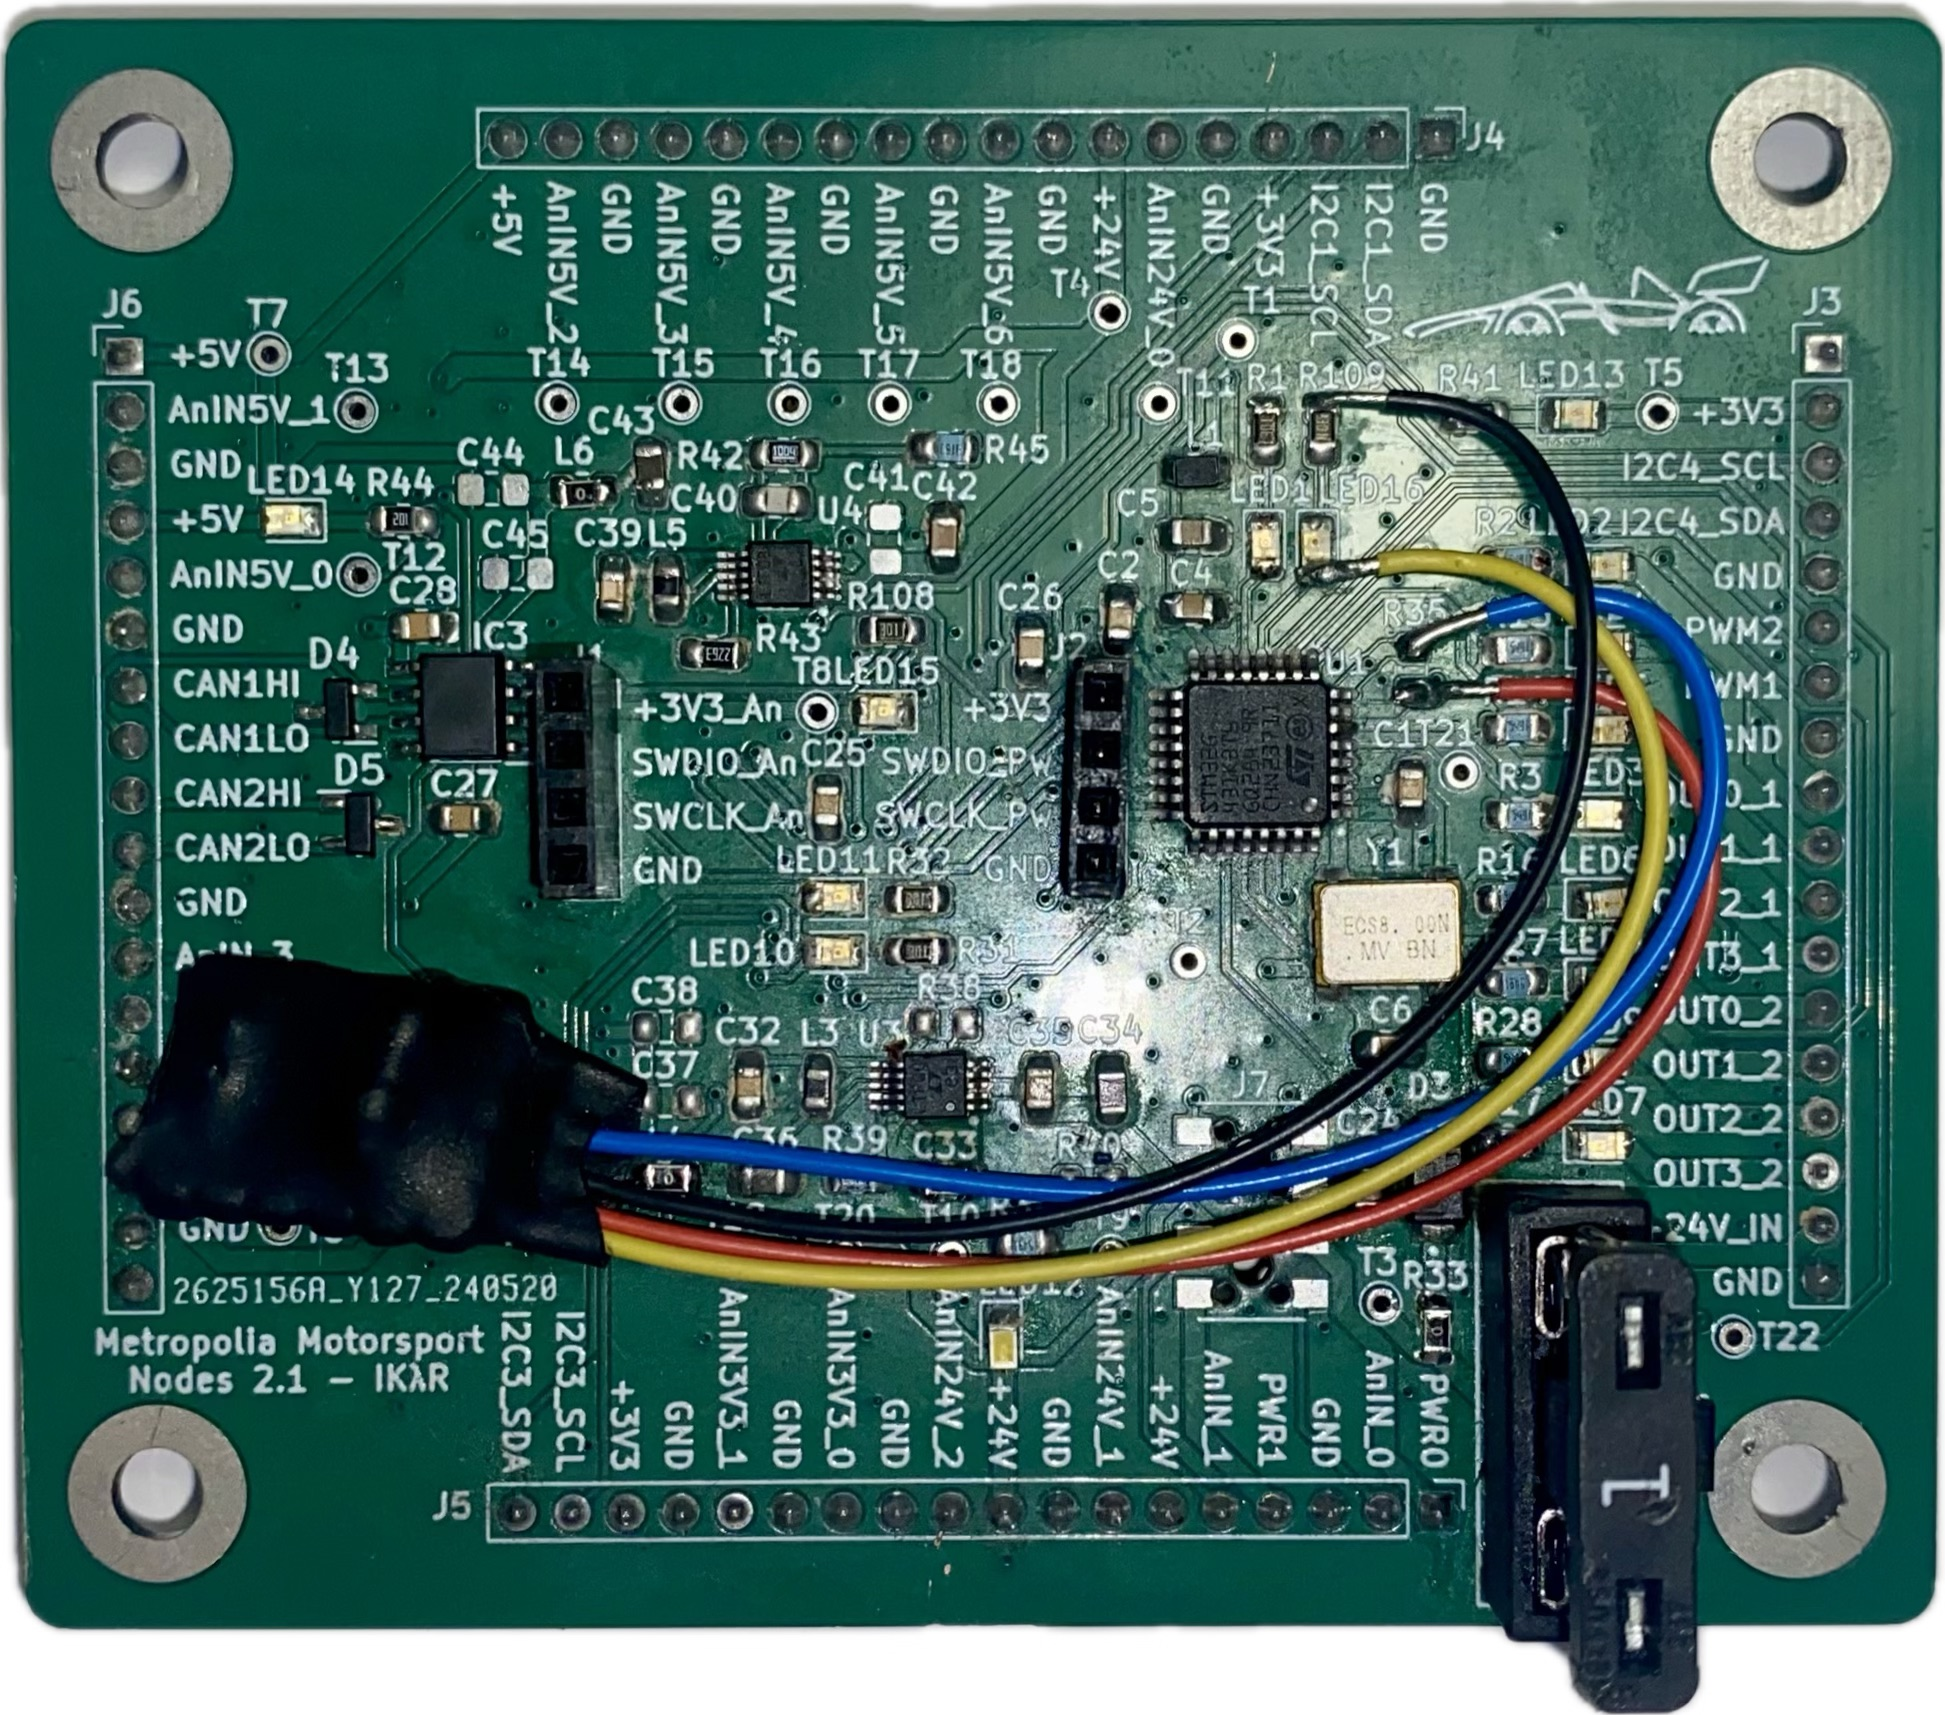
\includegraphics[width=0.45\linewidth]{Nodes_Front_v2.1.jpeg}
    \caption{Nodes v2.1 Board Front Side}
    \label{fig:nodes_front}
\end{figure}

\begin{figure} [h]
    \centering
    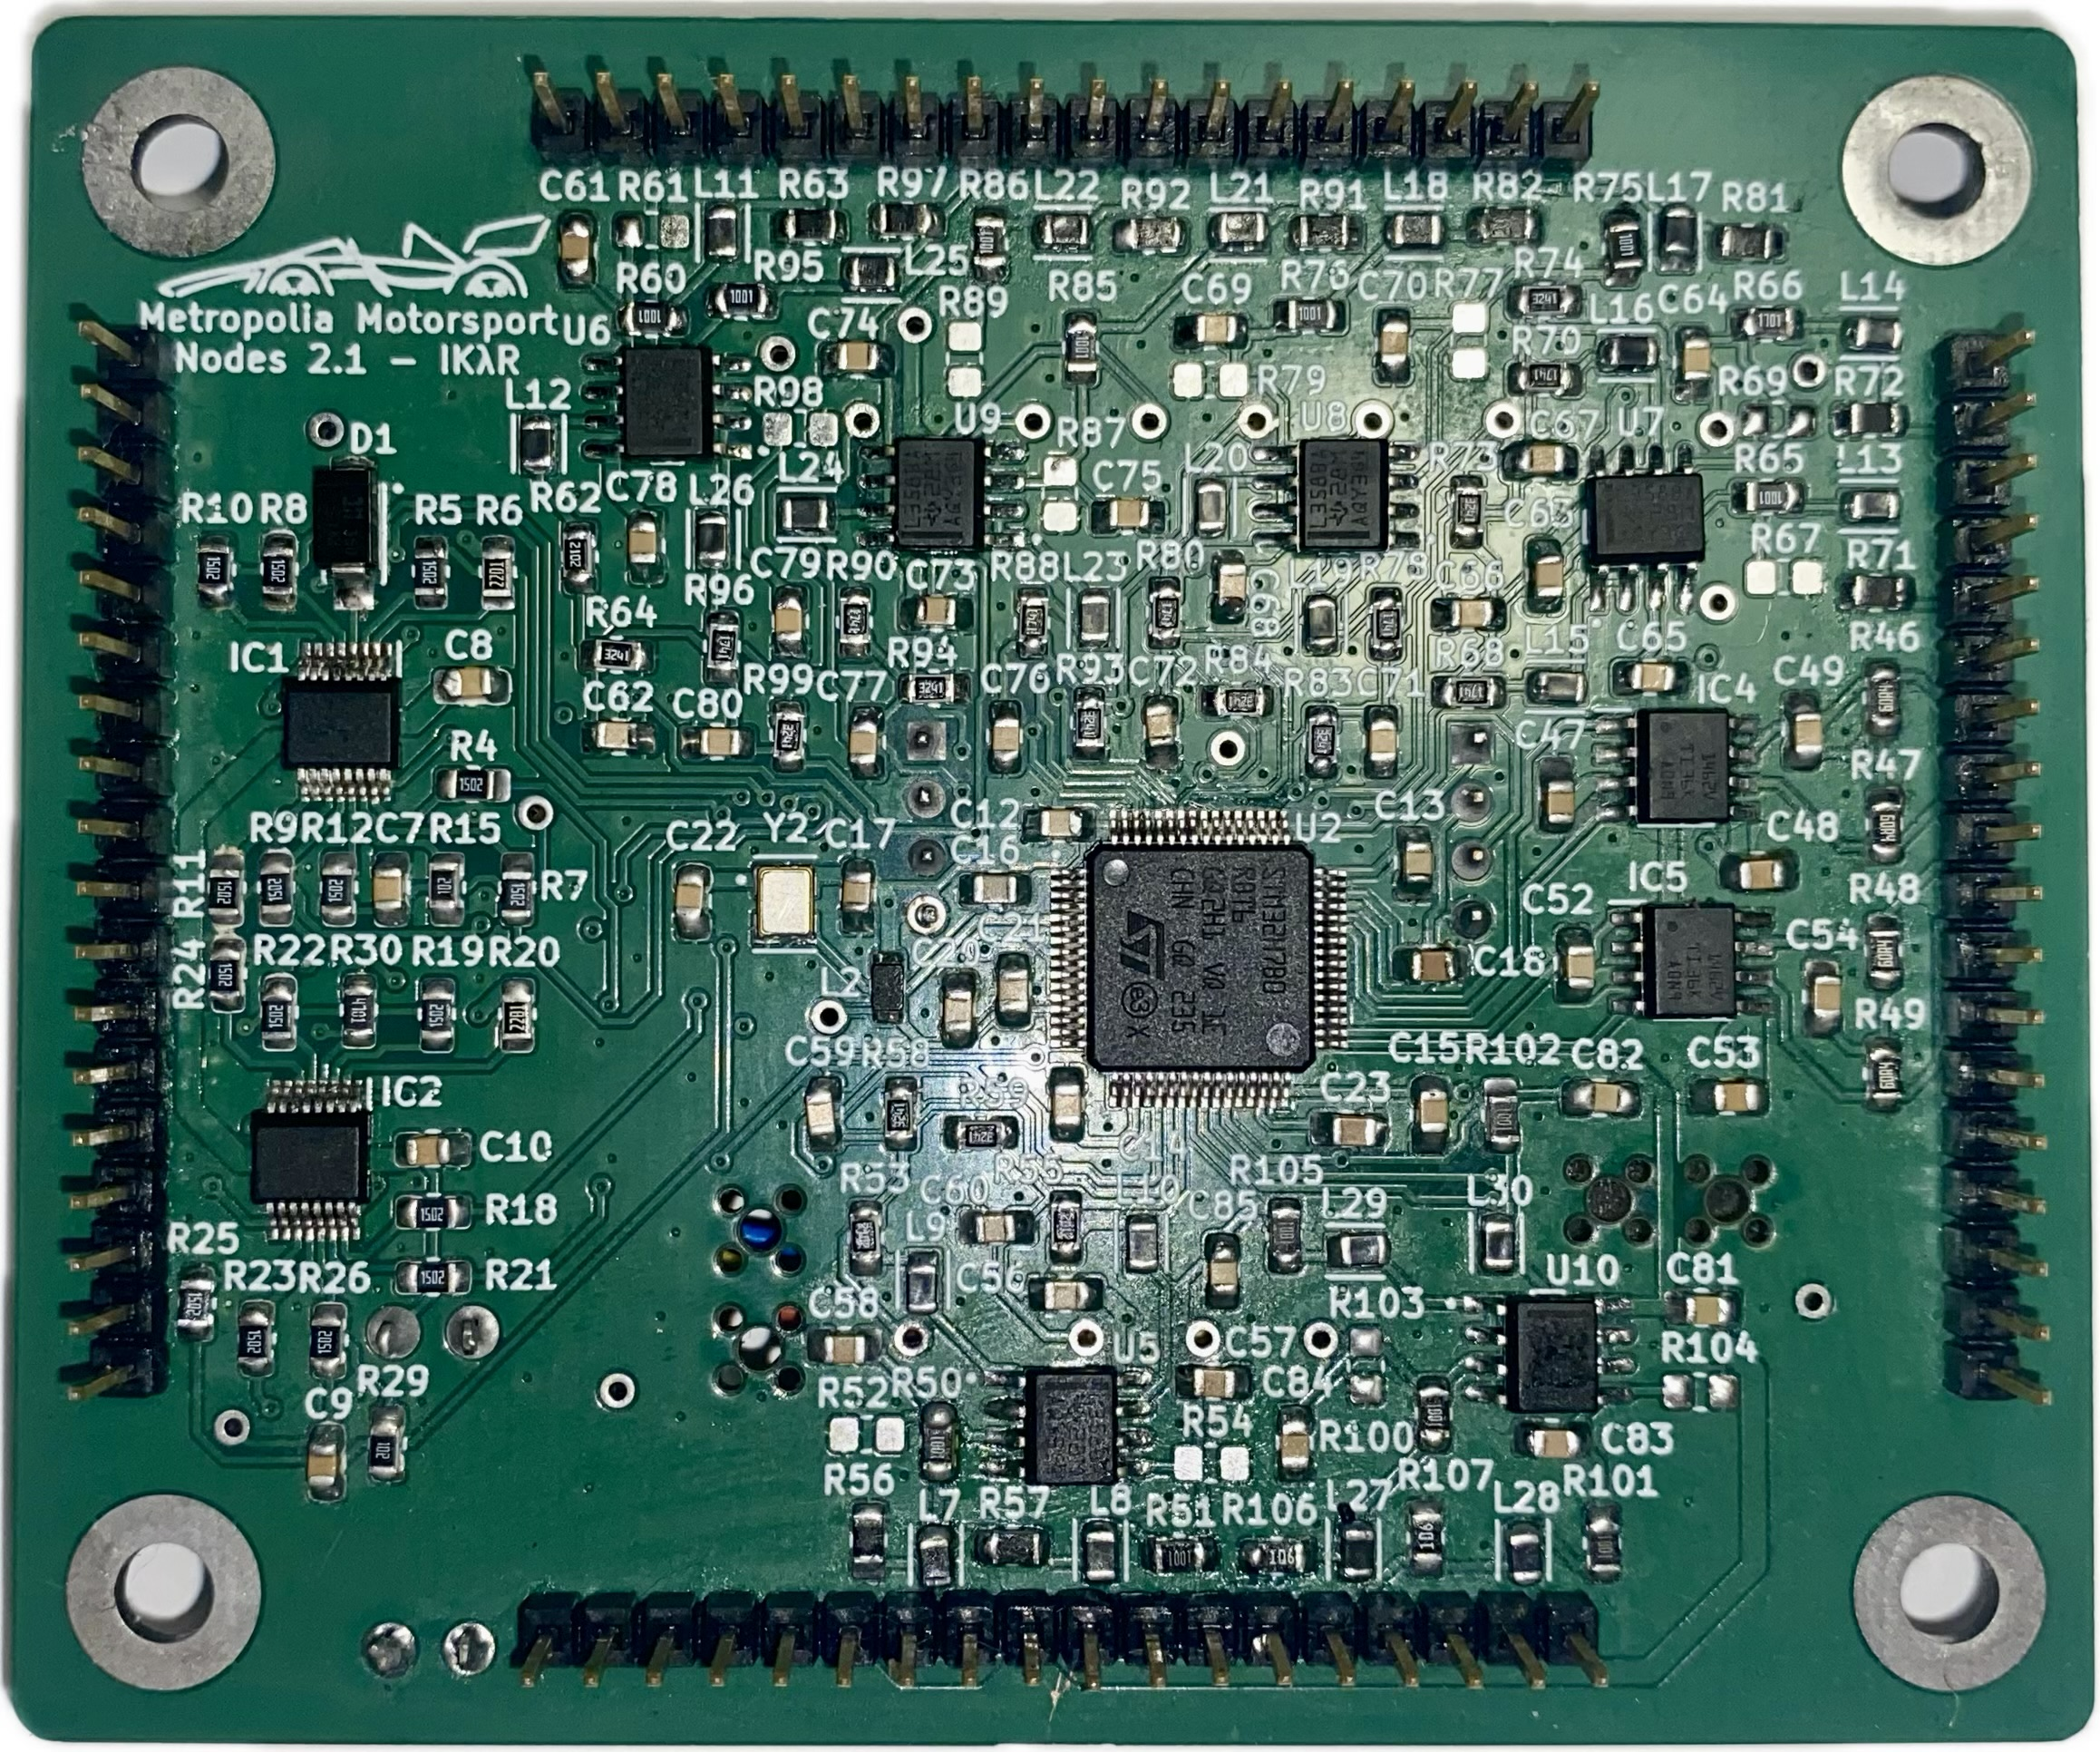
\includegraphics[width=0.45\linewidth]{Nodes_Back_v2.1.jpeg}
    \caption{Nodes v2.1 Board Back Side}
    \label{fig:nodes_back}
\end{figure}

% For wide tables, a single column layout is better. It can be switched
% page-by-page.
\onecolumn
\tableofcontents
\newpage

\section{Introduction}
{This datasheet covers all available information on the new Nodes design such as description, overview, electrical characteristics, pin assignment and definition, software. The document itself can be divided into two main parts, which consist of data about the board itself at the electronic level, as well as data regarding the software part.\\\\ 
The new version of Nodes was developed for Metropolia Motorsport and is under constant improvement and updating, so this datasheet should be constantly updated in accordance with the changes, so be careful when choosing the right version of the datasheet to avoid unexpected errors and problems. \\\\
This document mainly covers the stable version of Nodes v2.1, which at the time of writing the document is actively used, but the datasheet also contains references and clarifications of the new version 2.2, which was under development and was supposed to replace 2.1.\\\\
If the data written in this datasheet is insufficient and forces to explore additional sources of information, this means that it is necessary to supplement the documentation with the missing data, so report this situation to the person responsible for updating this documentation.}
\newpage
\section{Overview}
\label{overview}
Nodes are inherently an incredible combination of software and a variety of pre-existing components on the market, such as voltage regulators, microchips, operational amplifiers, high-side drivers and others, so it is very important to understand at a basic level what is happening in each part of the board in order to avoid various problems.
\subsection{Power Supply}
\label{ssec:power}
In order for Nodes to work reliably, high-quality and stable power is necessary not only for all components on the board, but also for additional connected equipment to the board, for example, sensors. To achieve this goal, a variety of solutions were implemented in Nodes. In both versions (2.1 and 2.2), the 24 volt input voltage is stabilized using diode \textit{D2}, zener diode \textit{D3} and capacitor \textit{C24} as shown in Figure \ref{fig:power}. As a result of the voltage passing through diode \textit{D2}, a voltage drop occurs by the value $V_f$, which is presented in Table \ref{table:elec_char}. The board is also protected from high current consumption with popular blade fuse 1A.
\begin{figure} [h]
    \centering
    
\includegraphics[width=0.45\linewidth]{Datasheet_electronics/Power.png}
    \caption{Voltage stabilization for 24V}
    \label{fig:power}
\end{figure} \\
Resistor \textit{R33} is used to measure the current consumption of the entire board using two test points \textit{T3} and \textit{T4} directly on the board without disconnecting anything. To do this, take a multimeter, put it in voltage measurement mode, and connect it to these test points with two wires, thereby you can get the voltage value through resistor \textit{R33}, in order to convert this into a current value, divide this value by the resistance of the resistor in accordance with the law Ohm, namely, perform the calculation of the Formula \ref{eq:current_res}.
\begin{equation}
\label{eq:current_res}
I_c=V_R/(10*10^{-3})
\end{equation}
Measuring current consumption for Analog Node through resistor \textit{R35} works in the same way; more information about this in Section \nameref{ssec:power_node}. \\
\newpage
\subsubsection{Voltage Regulators v2.1}
\label{sssec:vol_reg_v21}
After stabilization in version 2.1, 24V turns into 5V (Figure \ref{fig:power5v_v21}) and 3.3V (Figure \ref{fig:power3v3_v21}) using switching regulators. 5V powers the components for CAN and is used for output power, and 3.3V powers almost all components on the board and also provides output voltage. This version uses the LT3970\cite{ref4} as the main voltage regulator, which has been used in many Metropolia Motorsport projects for a long time.
\begin{figure} [h]
    \centering
    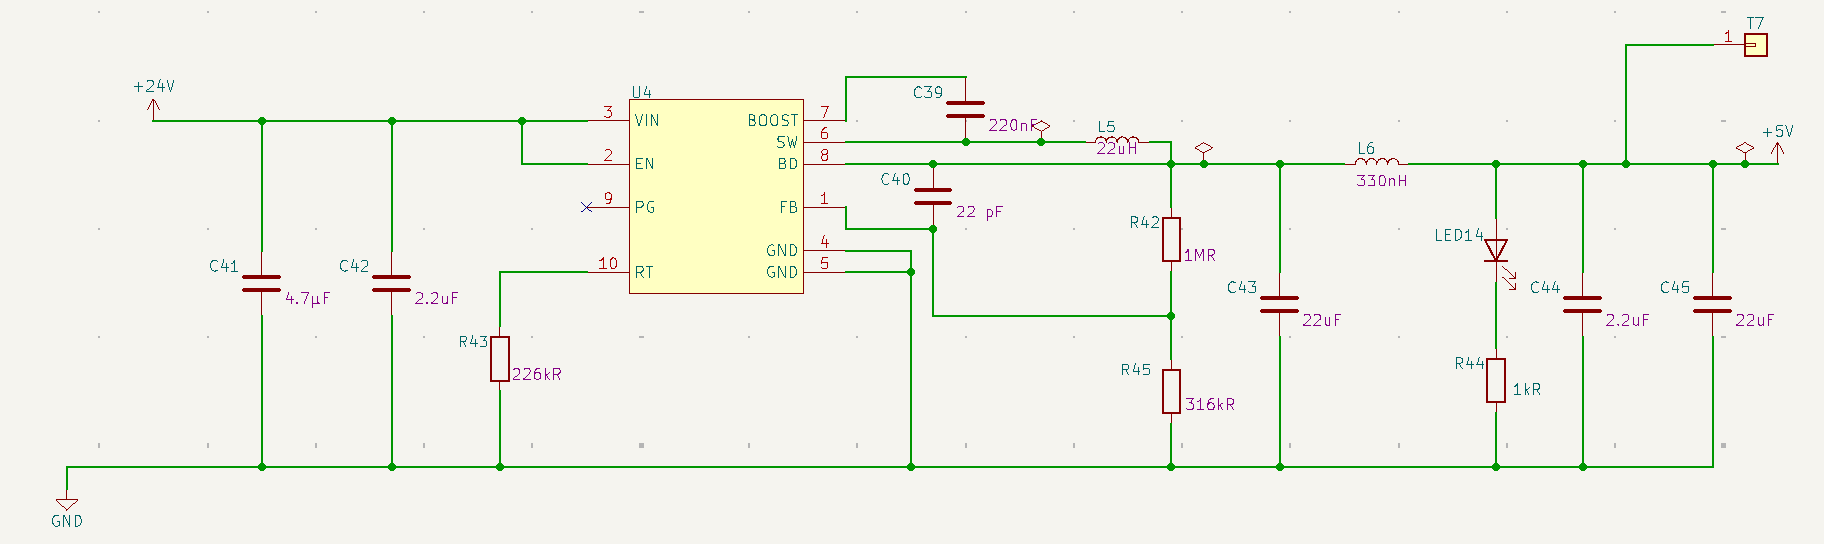
\includegraphics[width=0.6\linewidth]{Power5v_v21.png}
    \caption{Voltage regulator\cite{ref4} adj. schematic v2.1 for 5V}
    \label{fig:power5v_v21}
\end{figure} 
\begin{figure} [h]
    \centering
    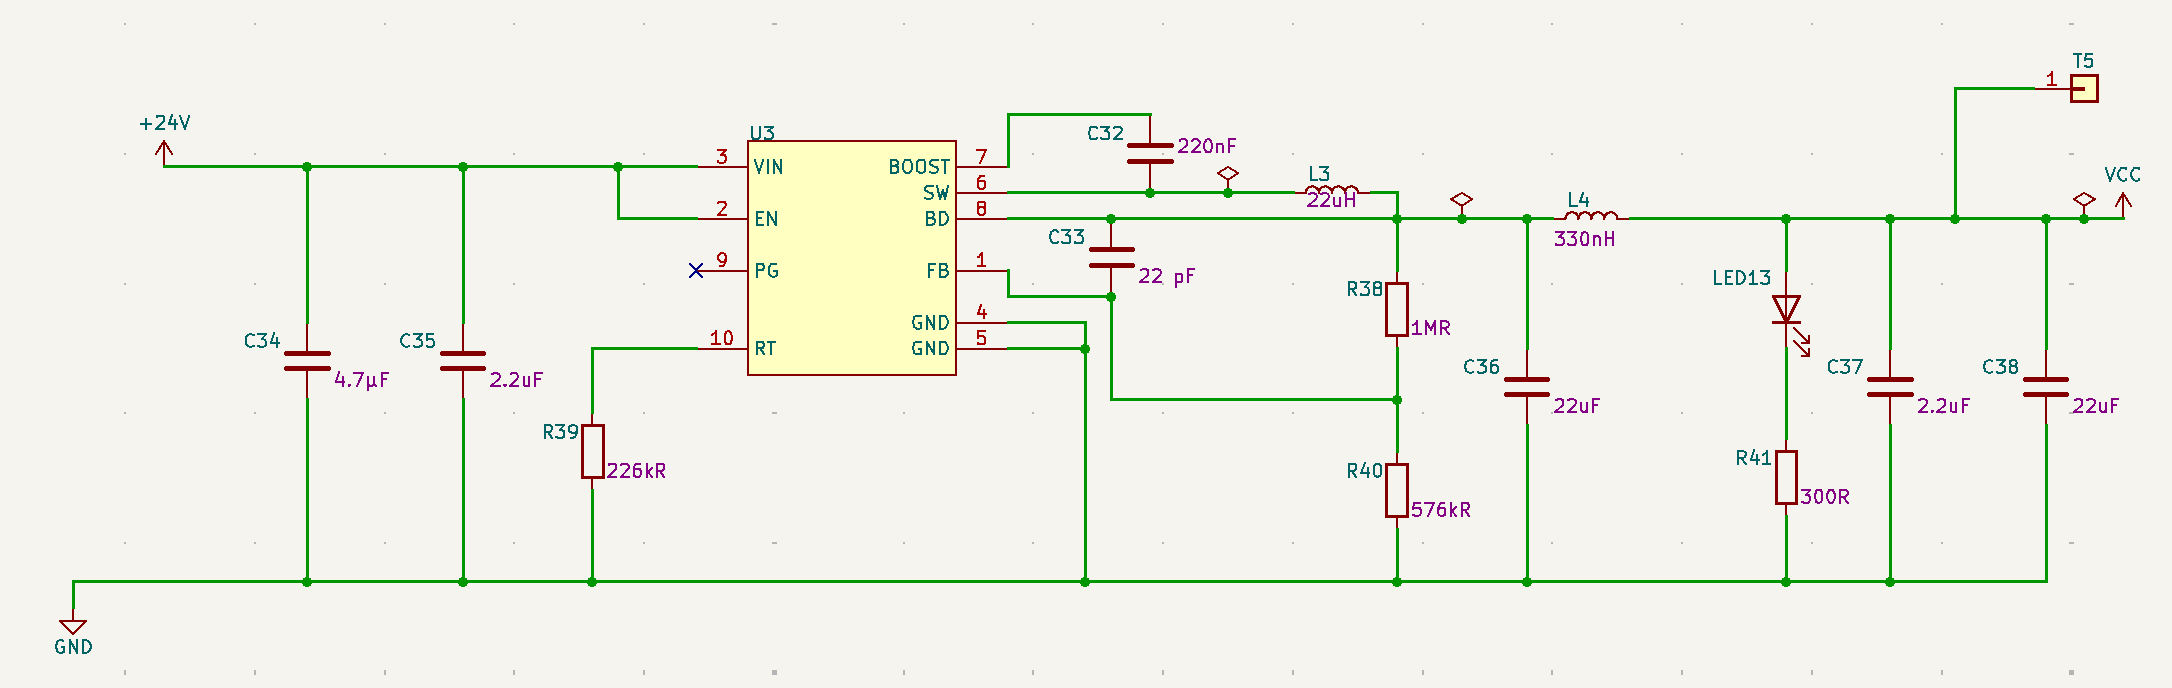
\includegraphics[width=0.6\linewidth]{Power3v3_v21.png}
    \caption{Voltage regulator\cite{ref4} adj. schematic v2.1 for 3.3V}
    \label{fig:power3v3_v21}
\end{figure} 
\\
Some components that are located near the voltage regulators are optional and are not dictated by the datasheet, namely for the 5V voltage regulator: C41, C44, C45 and L6 (L6 can be replaced with a jumper); for a 3.3V voltage regulator: C34, C37, C38 and L4 (L4 can be replaced with a jumper).\\
Also, the output voltage can be recalculated using Formula \ref{eq:voltage_out}, in which the values of $R_h$ and $R_l$ could be replaced by (\textit{R42} and \textit{R45}) or (\textit{R38} or \textit{R40}) respectively.
\begin{equation}
\label{eq:voltage_out}
V_{out}=1.2*(1+R_h/R_l)
\end{equation}
Based on practical experience, it is recommended to use non-adjustable power components to achieve maximum stability of the result. To use the non-adjustable version of the voltage regulator, some components must be removed. \\ 
In the case of 5V, remove \textit{C40} and \textit{R45}, but also replace \textit{R42} with a zero resistor. \\
In the case of 3.3V, remove \textit{C33} and \textit{R40}, but also replace \textit{R38} with a zero resistor, so that the resulting connection looks like in the Figure \ref{fig:non-adjustable_lt3970}.
\begin{figure} [h]
    \centering
    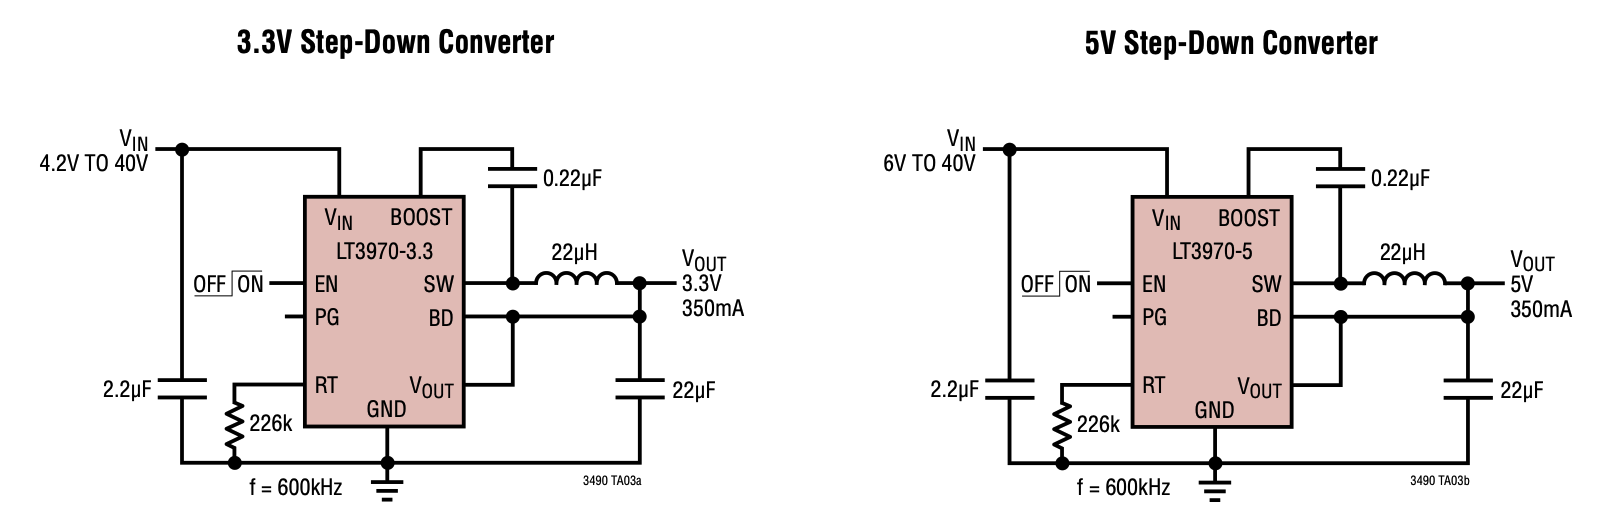
\includegraphics[width=0.6\linewidth]{Non-adjustable_LT3970.png}
    \caption{Non-adjustable LT3970 schematics\cite{ref4}}
    \label{fig:non-adjustable_lt3970}
\end{figure} \\
Over a long period of use, a large number of complaints were collected about this component, such as soldering, reliability, number of additional components, price, etc., so it was decided to find another power solution.
\newpage
\subsubsection{Voltage Regulators v2.2}
\label{sssec:vol_reg_v22}
In version 2.2, the LMR50410-Q1\cite{ref6} is used as a voltage regulator, which at the time of writing the datasheet seemed the most suitable, given the complaints of the previous version. In this version, there is only one switching regulator on the board, which converts 24V to 5V as shown in Figure \ref{fig:power5v_v22}. \\
The circuit below on the Figure \ref{fig:power5v_v22} is for an adjustable version (LMR50410YFQDBVRQ1).
And the output voltage can be recalculated using Formula \ref{eq:voltage_out_swr}.
\begin{equation}
\label{eq:voltage_out_swr}
V_{out}=1+R_{48}/R_{49}
\end{equation}
It is recommended to use a fixed voltage regulator (LMR50410Y5FQDBVRQ1). \\
In order for the circuit to be suitable for a fixed regulator, it is necessary to connect the FB pin to the SW pin directly, so for this remove \textit{R49}, and solder a jumper in place of \textit{R48}.
\begin{figure} [h]
    \centering
    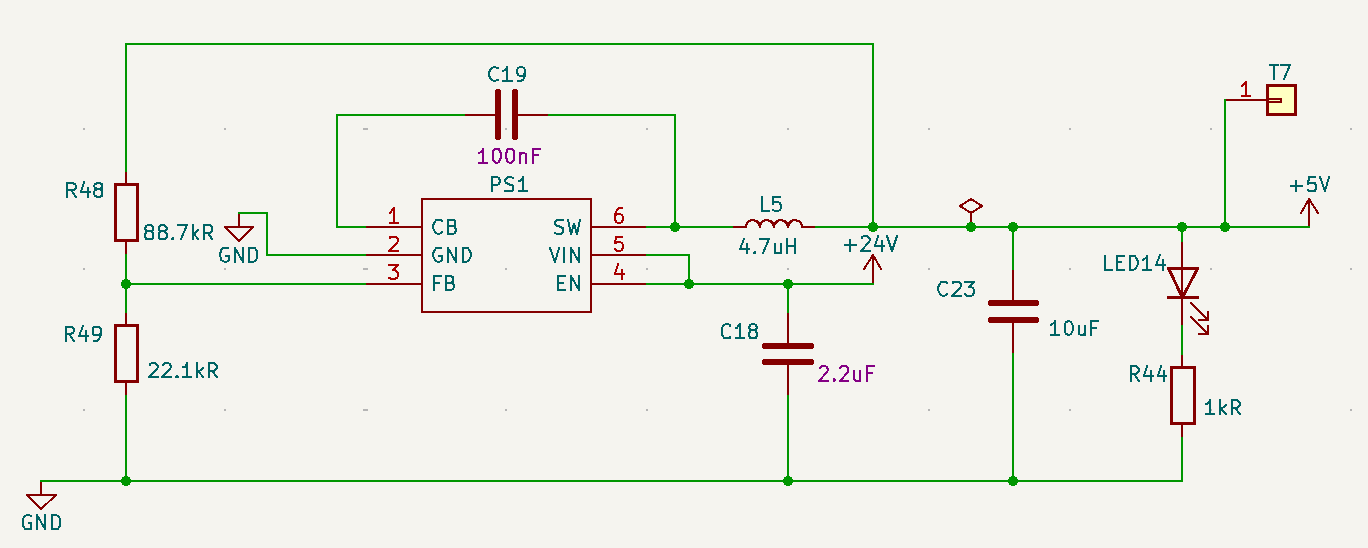
\includegraphics[width=0.7\linewidth]{Power5v_v22.png}
    \caption{Voltage regulator\cite{ref6} adj. schematic v2.2 for 5V}
    \label{fig:power5v_v22}
\end{figure} \\
The 5V is then converted to 3.3V using the ST730\cite{ref5} linear regulator to provide even greater 3.3V voltage stability especially for Analog part components (Figure \ref{fig:power3v3_v22}). \\
The circuit below on the Figure \ref{fig:power3v3_v22} is for an adjustable version (ST730MR). If an adjustable version of the component is used, in this case it is recommended to use the Formula \ref{eq:voltage_out} to calculate output voltage, where $R_h$ is \textit{R42} and $R_l$ is \textit{R43}. \\
It is recommended to use a fixed voltage regulator (ST730M33R). \\
In order for the circuit to be suitable for a fixed regulator, remove \textit{R42} and \textit{R43}. \\
\begin{figure} [h]
    \centering
    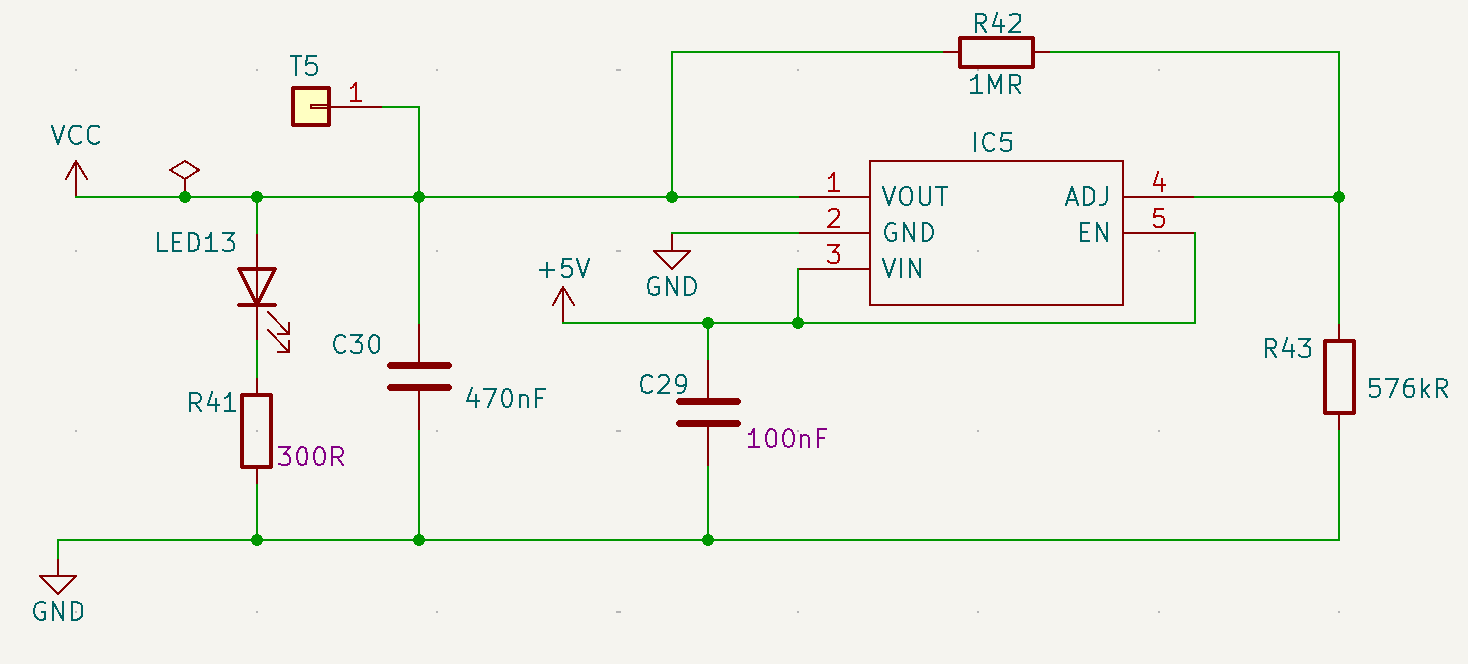
\includegraphics[width=0.7\linewidth]{Power3v3_v22.png}
    \caption{Voltage regulator\cite{ref5} adj. schematic v2.2 for 3.3V}
    \label{fig:power3v3_v22}
\end{figure} \\
It is worth noting that there are two such LDOs on the board and one of them is controlled using the \textit{U1} chip on the Power Node part to control power for the Analog Node. More data on controlled power supply for Analog Node is presented in the next section.
\newpage
\subsubsection{Controllable Power for Analog Node}
\label{sssec:control_power}
To be sure of the operation of each part of the Nodes, the control over them is needed, and for this purpose the controllable power supply for Analog Nodes was implemented. In the case of version 2.1, this decision was also caused by the fact that the chip for the Analog Node, unlike the Power Node, was unstable when power was directly connected to it, so the solution with the switch, as shown in the Figure \ref{fig:power3v3_An_v21}, could be described as forced. \\ 
But a little later, as a result of conducting numerous tests, it was discovered that the solution with the switch is not a solution to a specific problem, but a treatment for the symptoms caused by it. More information could be found in the Section \nameref{ssec:power_node}.  \\
% At the time of writing this section, the exact cause of this phenomenon is unknown. Perhaps it’s all about the chip itself and its subtleties of operation, which were not fully taken into account when developing the design, or the LT3970 voltage regulator, which, as mentioned earlier in Section \nameref{sssec:vol_reg_v21}, is extremely sensitive and requires special attention when using it. \\
In the oldest version of 2.1, the power switch TPS22995HQDDCRQ1\cite{ref7} is not present on the board layout itself, so a separate board was developed, which was soldered into the necessary places (Red Wire - 3.3V; Black Wire - GND; Yellow Wire - Control Signal from Power Node or on the board LED 16; Blue Wire - 3.3V\_An), as shown in the Figure \ref{fig:nodes_front}.
\begin{figure} [h]
    \centering
    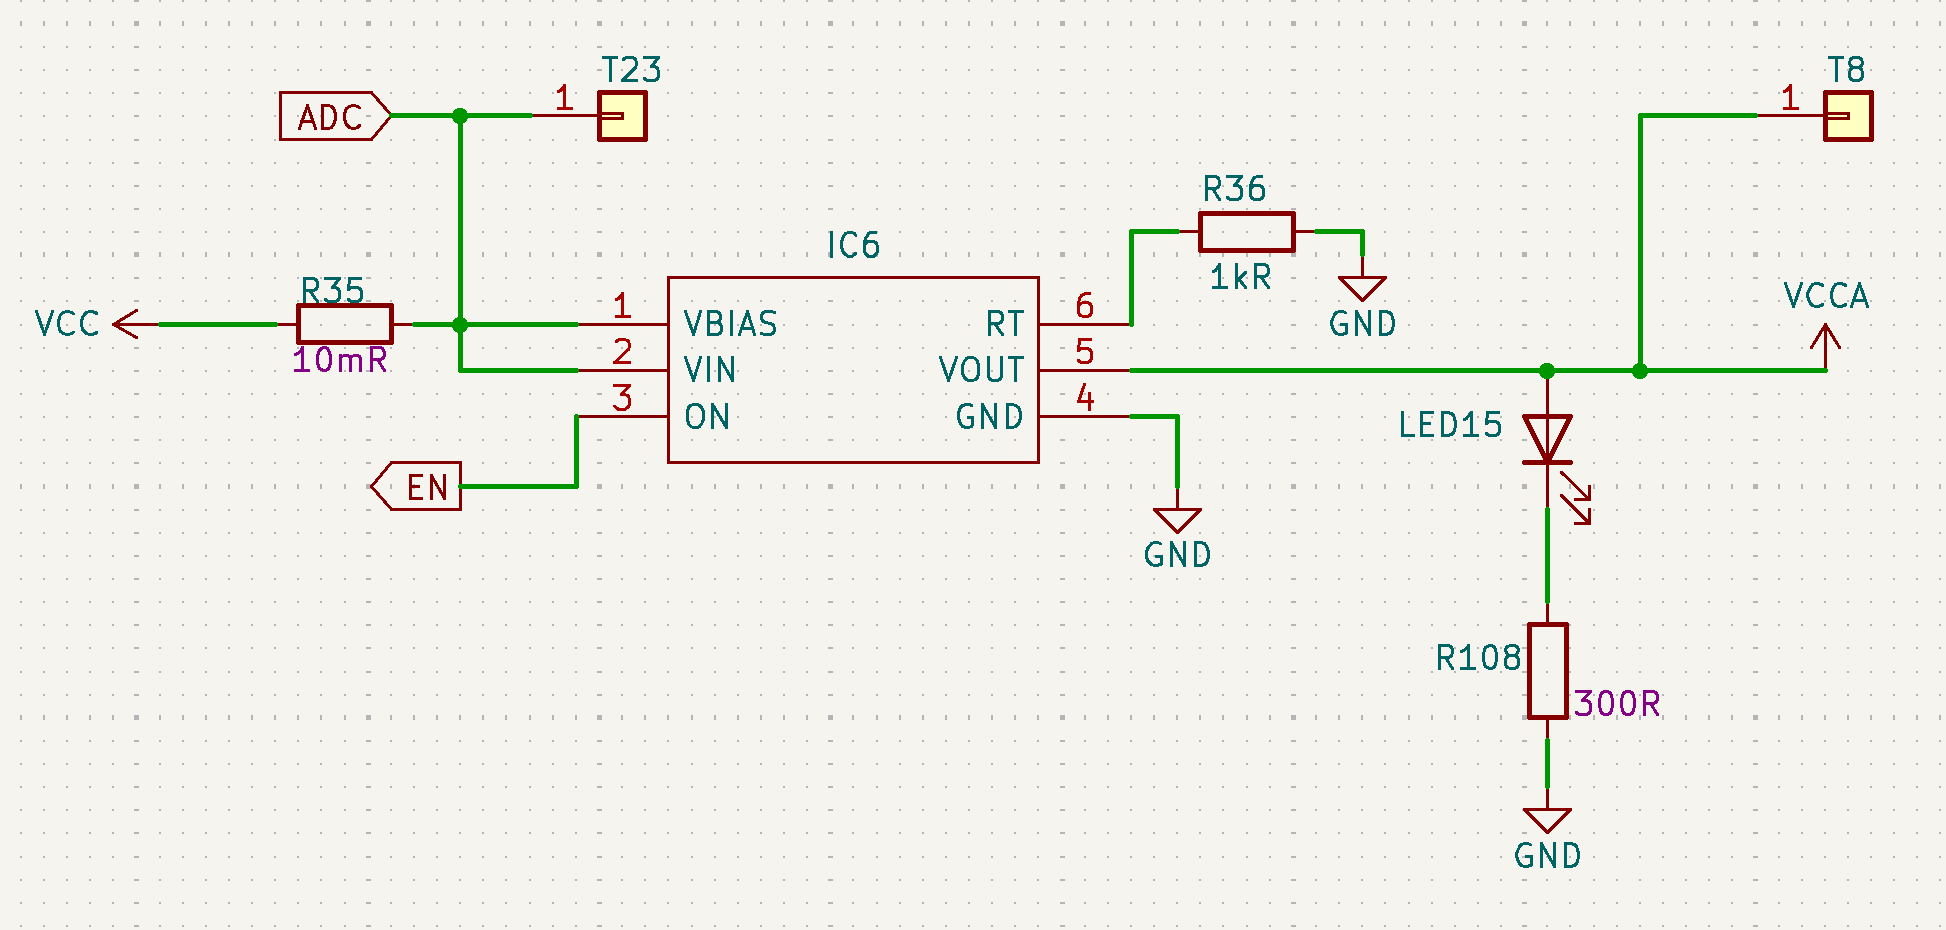
\includegraphics[width=0.55\linewidth]{power3v3_An_v21.png}
    \caption{Power Switch\cite{ref7} for Analog Node power schematic v2.1}
    \label{fig:power3v3_An_v21}
\end{figure}
\\
Therefore, in the new version 2.2, it was decided to rework the power system, as well as choose a new chip for the Analog Node from the same STM32G4 series as the Power Node, which showed its best side during numerous tests and operations. So the power supply for the Analog Node in this version is not controlled by a separate switch, but by a separate linear voltage regulator\cite{ref5}, which has EN (enable) pin (Figure \ref{fig:power3v3_An_v22}). \\
The circuit generally follows the pattern shown in Figure \ref{fig:power3v3_v22}, with some exceptions. Therefore, here it is also possible to use non-adjustable version with small changes.\\
The circuit below on the Figure \ref{fig:power3v3_An_v22} is for an adjustable version (ST730MR). If an adjustable version of the component is used, in this case it is recommended to use the Formula \ref{eq:voltage_out} to calculate output voltage, where $R_h$ is \textit{R39} and $R_l$ is \textit{R40}. \\
It is recommended to use a fixed voltage regulator (ST730M33R). \\
In order for the circuit to be suitable for a fixed regulator, remove \textit{R39} and \textit{R40}.
\begin{figure} [h]
    \centering
    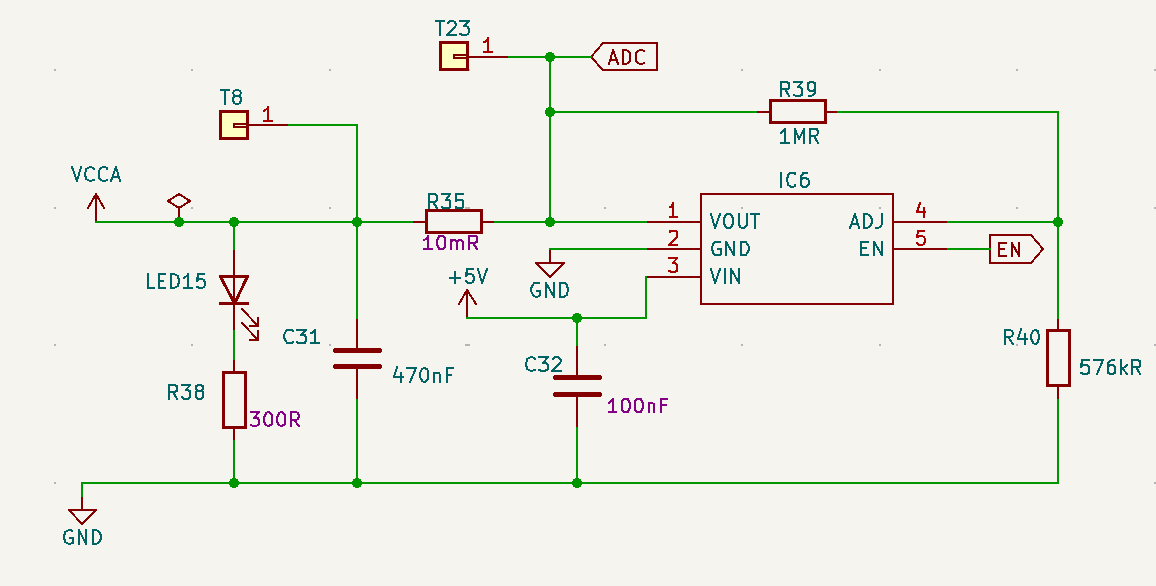
\includegraphics[width=0.55\linewidth]{Power3v3_An_v22.png}
    \caption{Voltage regulator\cite{ref5} adj. for Analog Node part schematic v2.2 for 3.3V}
    \label{fig:power3v3_An_v22}
\end{figure}
\newpage
\subsection{Power Node}
\label{ssec:power_node}
One of the key parts of the Nodes is the Power Node, which is capable of controlling 24V power for a variety of parts of the car and monitoring their condition with CAN, as well as generating a PWM signal, which is necessary for pumps and fans. The center of it all is the STM32G431KBT6\cite{ref8} (\textit{U1}) chip. This chip is quite reliable and showed its best performance after numerous tests. \\
In the Section \nameref{sssec:control_power} Power Node actually controls using the EN pin, and also measures the current consumption on this part of the board using pins PA2 and PA3.\\
Versions 2.1 and 2.2 differ minimally in this section, but the main difference is in how current consumption is measured on the Analog Node. In version 2.1, resistor \textit{R35}, with which the current was measured, was located in front of the switch (Figure \ref{fig:power3v3_An_v21}), and in version 2.2, resistor \textit{R35} is located after the voltage regulator (Figure \ref{fig:power3v3_An_v22}), which is dictated mainly by nuances associated with the design stage, as well as measurement points, because which seemed much more important to obtain consumption data without the voltage regulator itself. And how to measure current consumption through a resistor is mentioned in the beginning of Section \nameref{ssec:power}.
\begin{figure} [h]
    \centering
    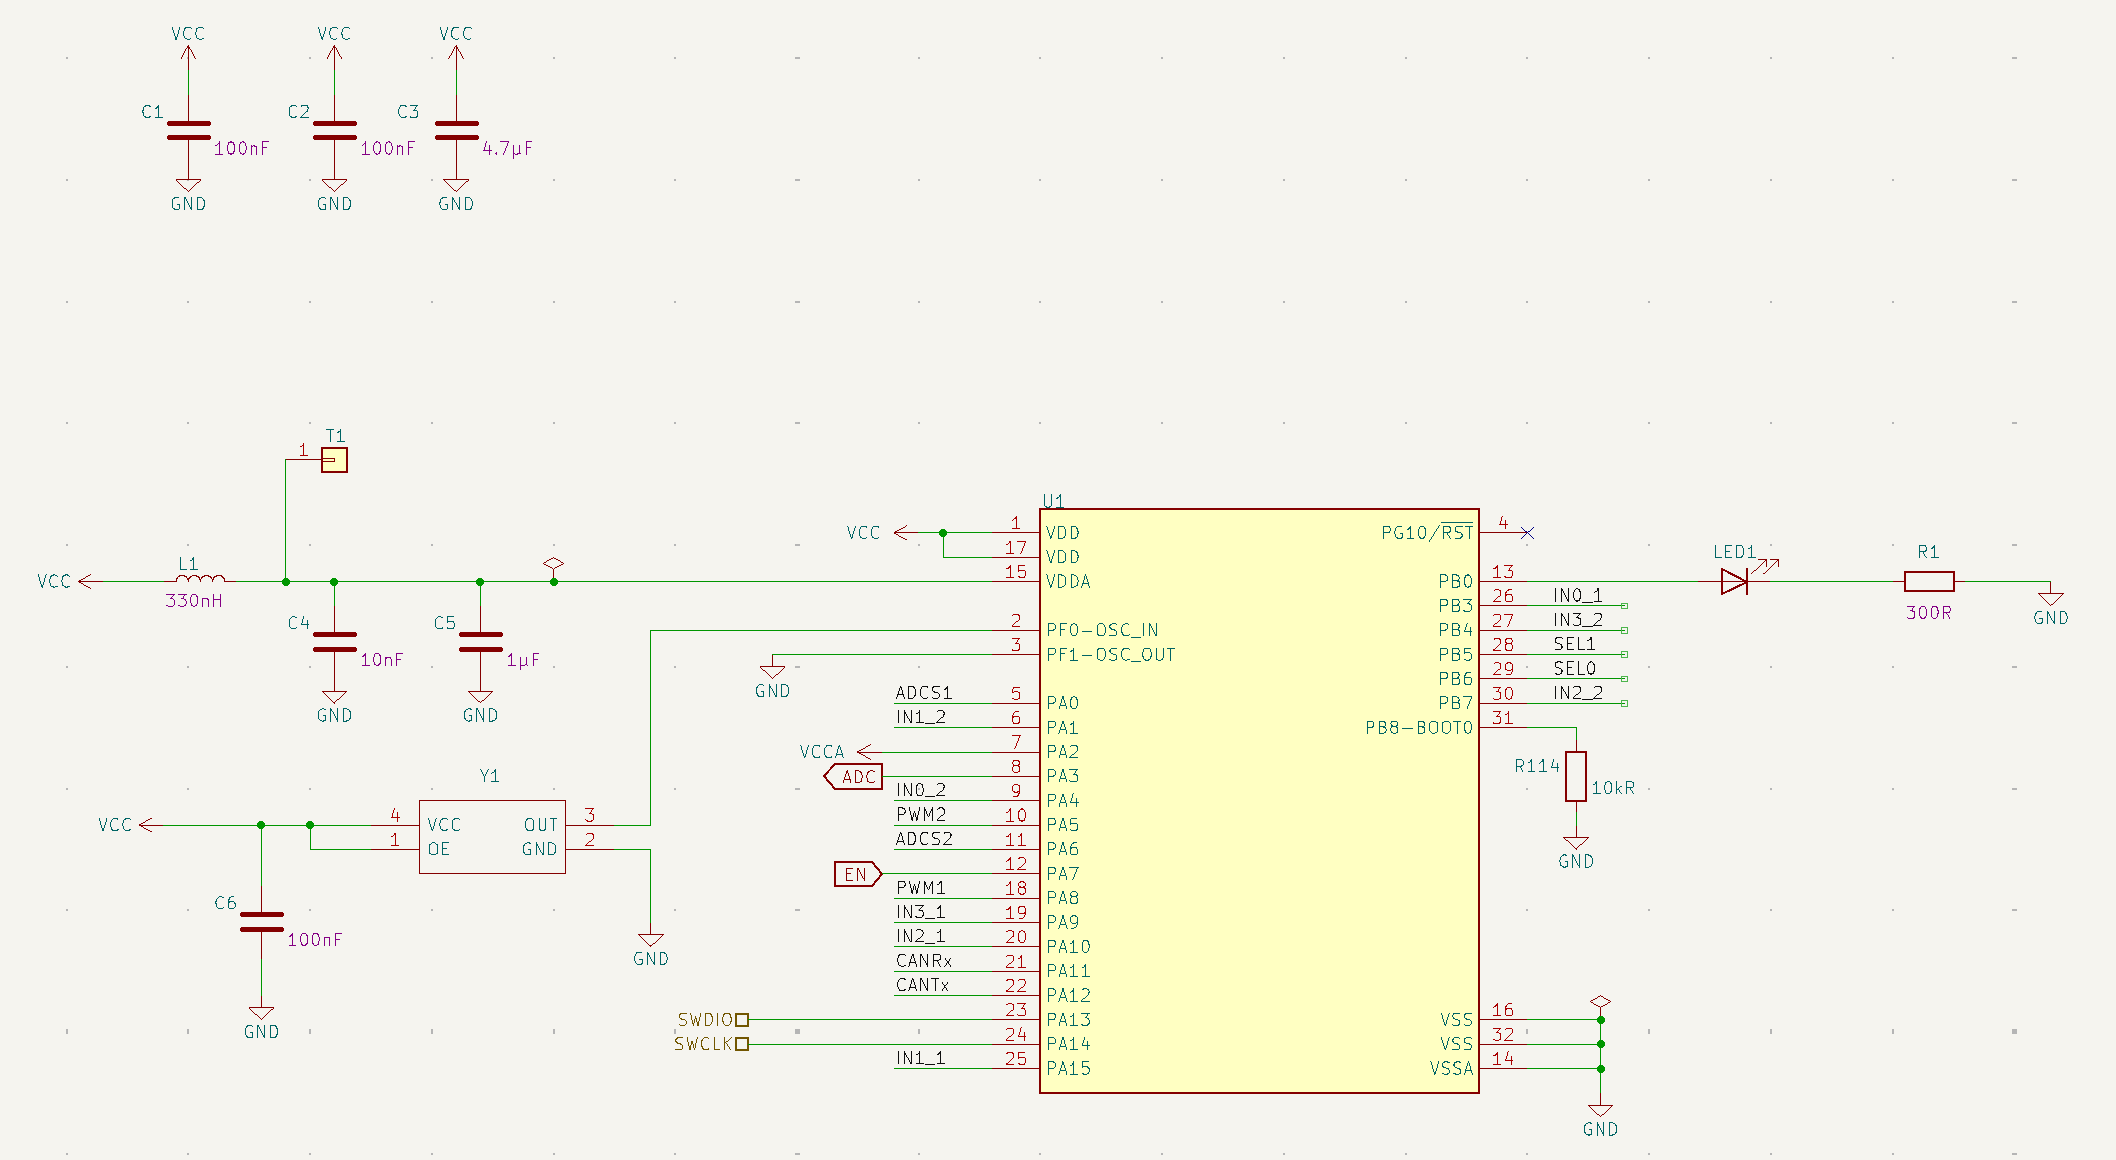
\includegraphics[width=1\linewidth]{Power_Node.png}
    \caption{Power Node schematic}
    \label{fig:power_node}
\end{figure} \\
For greater stability of the chip, an external oscillator (\textit{Y1}) is used. Power Node version 2.1 uses an oscillator ECS-7050MV-080-BN-TR\cite{ref9}, and version 2.2 uses the same one as the Analog Node SG-8018CE\_8.0000M-TJHPA3\cite{ref10}. Table 1 specifies the frequency range for the external oscillator, but a typical value is 8 MHz. If there is no oscillator with a typical frequency, it is possible to install another one in accordance with the frequency range and footprint sizes (For more information on footprint sizes, see the oscillator datasheet). When installing an oscillator with a different frequency, it is necessary to change the parameters in the code that relate to this, so it is worth notifying the person responsible for editing the code about the change in the oscillator frequency.\\
There is also a controllable LED (\textit{LED1})that can be used to monitor the operation of the chip and certain functions. More information about LEDs can be found in Section \nameref{ssec:led_code}.\\
There should be capacitors near the chip, which should be distributed as evenly as possible around the chip and as close to the pins as possible, all this is done in accordance with the datasheet of the chip itself. In general, this rule applies to all parts of the Nodes, namely, it is necessary to place components from common parts as close as possible to each other, so it is worth paying special attention to the location of particularly critical components on the board, since the stability of the entire board depends on this. The Power Node and Analog Node have a $V_{DDA}$ pin, which is used by the ADC as a reference, so the analog signal can be converted to digital. A small filter system consisting of an inductor and capacitors is connected to this pin.\\
It is also worth mentioning that there was a problem with unstable startup of the chip. The failure was previously solved by a banal restart of the power supply of the entire board, which was obviously not the best way. As it turned out later, the unstable operation of the chips during their startup was most likely caused not by unstable power supply, although this may have aggravated the situation, but by the fact that the BOOT pin of the chip remained floating, which, as it turned out, is not acceptable. Therefore, it is strongly recommended to solder a 10k pull-down resistor to each BOOT pin of the STM32 chip, if they are not used in some other way. In version 2.2.3 and newer, there is already a resistor \textit{R114} connected to the BOOT pin, so there is no longer a need to solder large resistors from the outside to solve this problem. \\
%It is also worth mentioning that when the board is started cold, that is, it was turned off for some time, then when power is supplied, the chip on the Power Node does not start correctly, for reasons that have not been precisely defined, and as a result of this the Analog Node does not start either. In this case, it is necessary to carry out a simple procedure, namely turn off and turn on the power. This helps in version 2.1 and older, but at the time of writing this issue should theoretically be fixed with the implementation of version 2.2. Further comments will be written later after testing the new version. \\
The chip in versions 2.1 and 2.2 is programmed using a JTAG, which consists of four pins, namely +3V3, SWDIO, SWCLK and GND, as shown in the Figure \ref{fig:jtag_power}. For programming, a special ST-LINK device is used, which is shown in the Figure \ref{fig:st-link}, and STM32CubeIDE software. Connect ST-LINK carefully, because it is possible to make a mistake when connecting and then the power will be connected to ground, which can lead to inevitable consequences.
\begin{figure} [h]
    \centering
    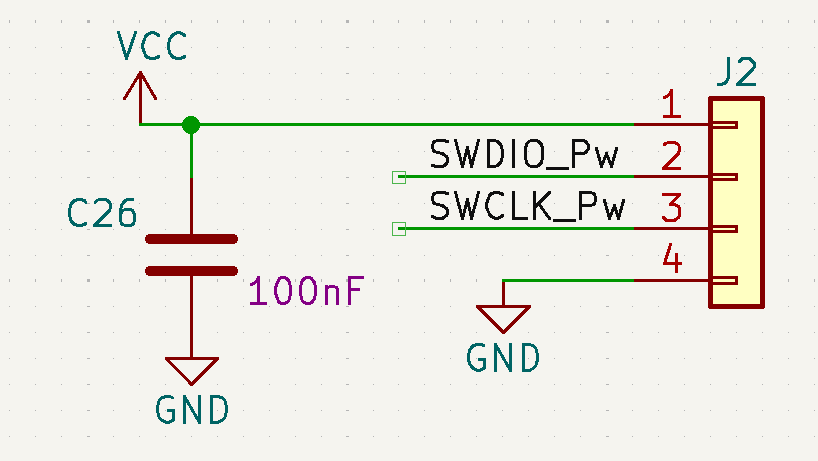
\includegraphics[width=0.5\linewidth]{JTAG_power.png}
    \caption{JTAG connector of the Power Node}
    \label{fig:jtag_power}
\end{figure}
\begin{figure} [h]
    \centering
    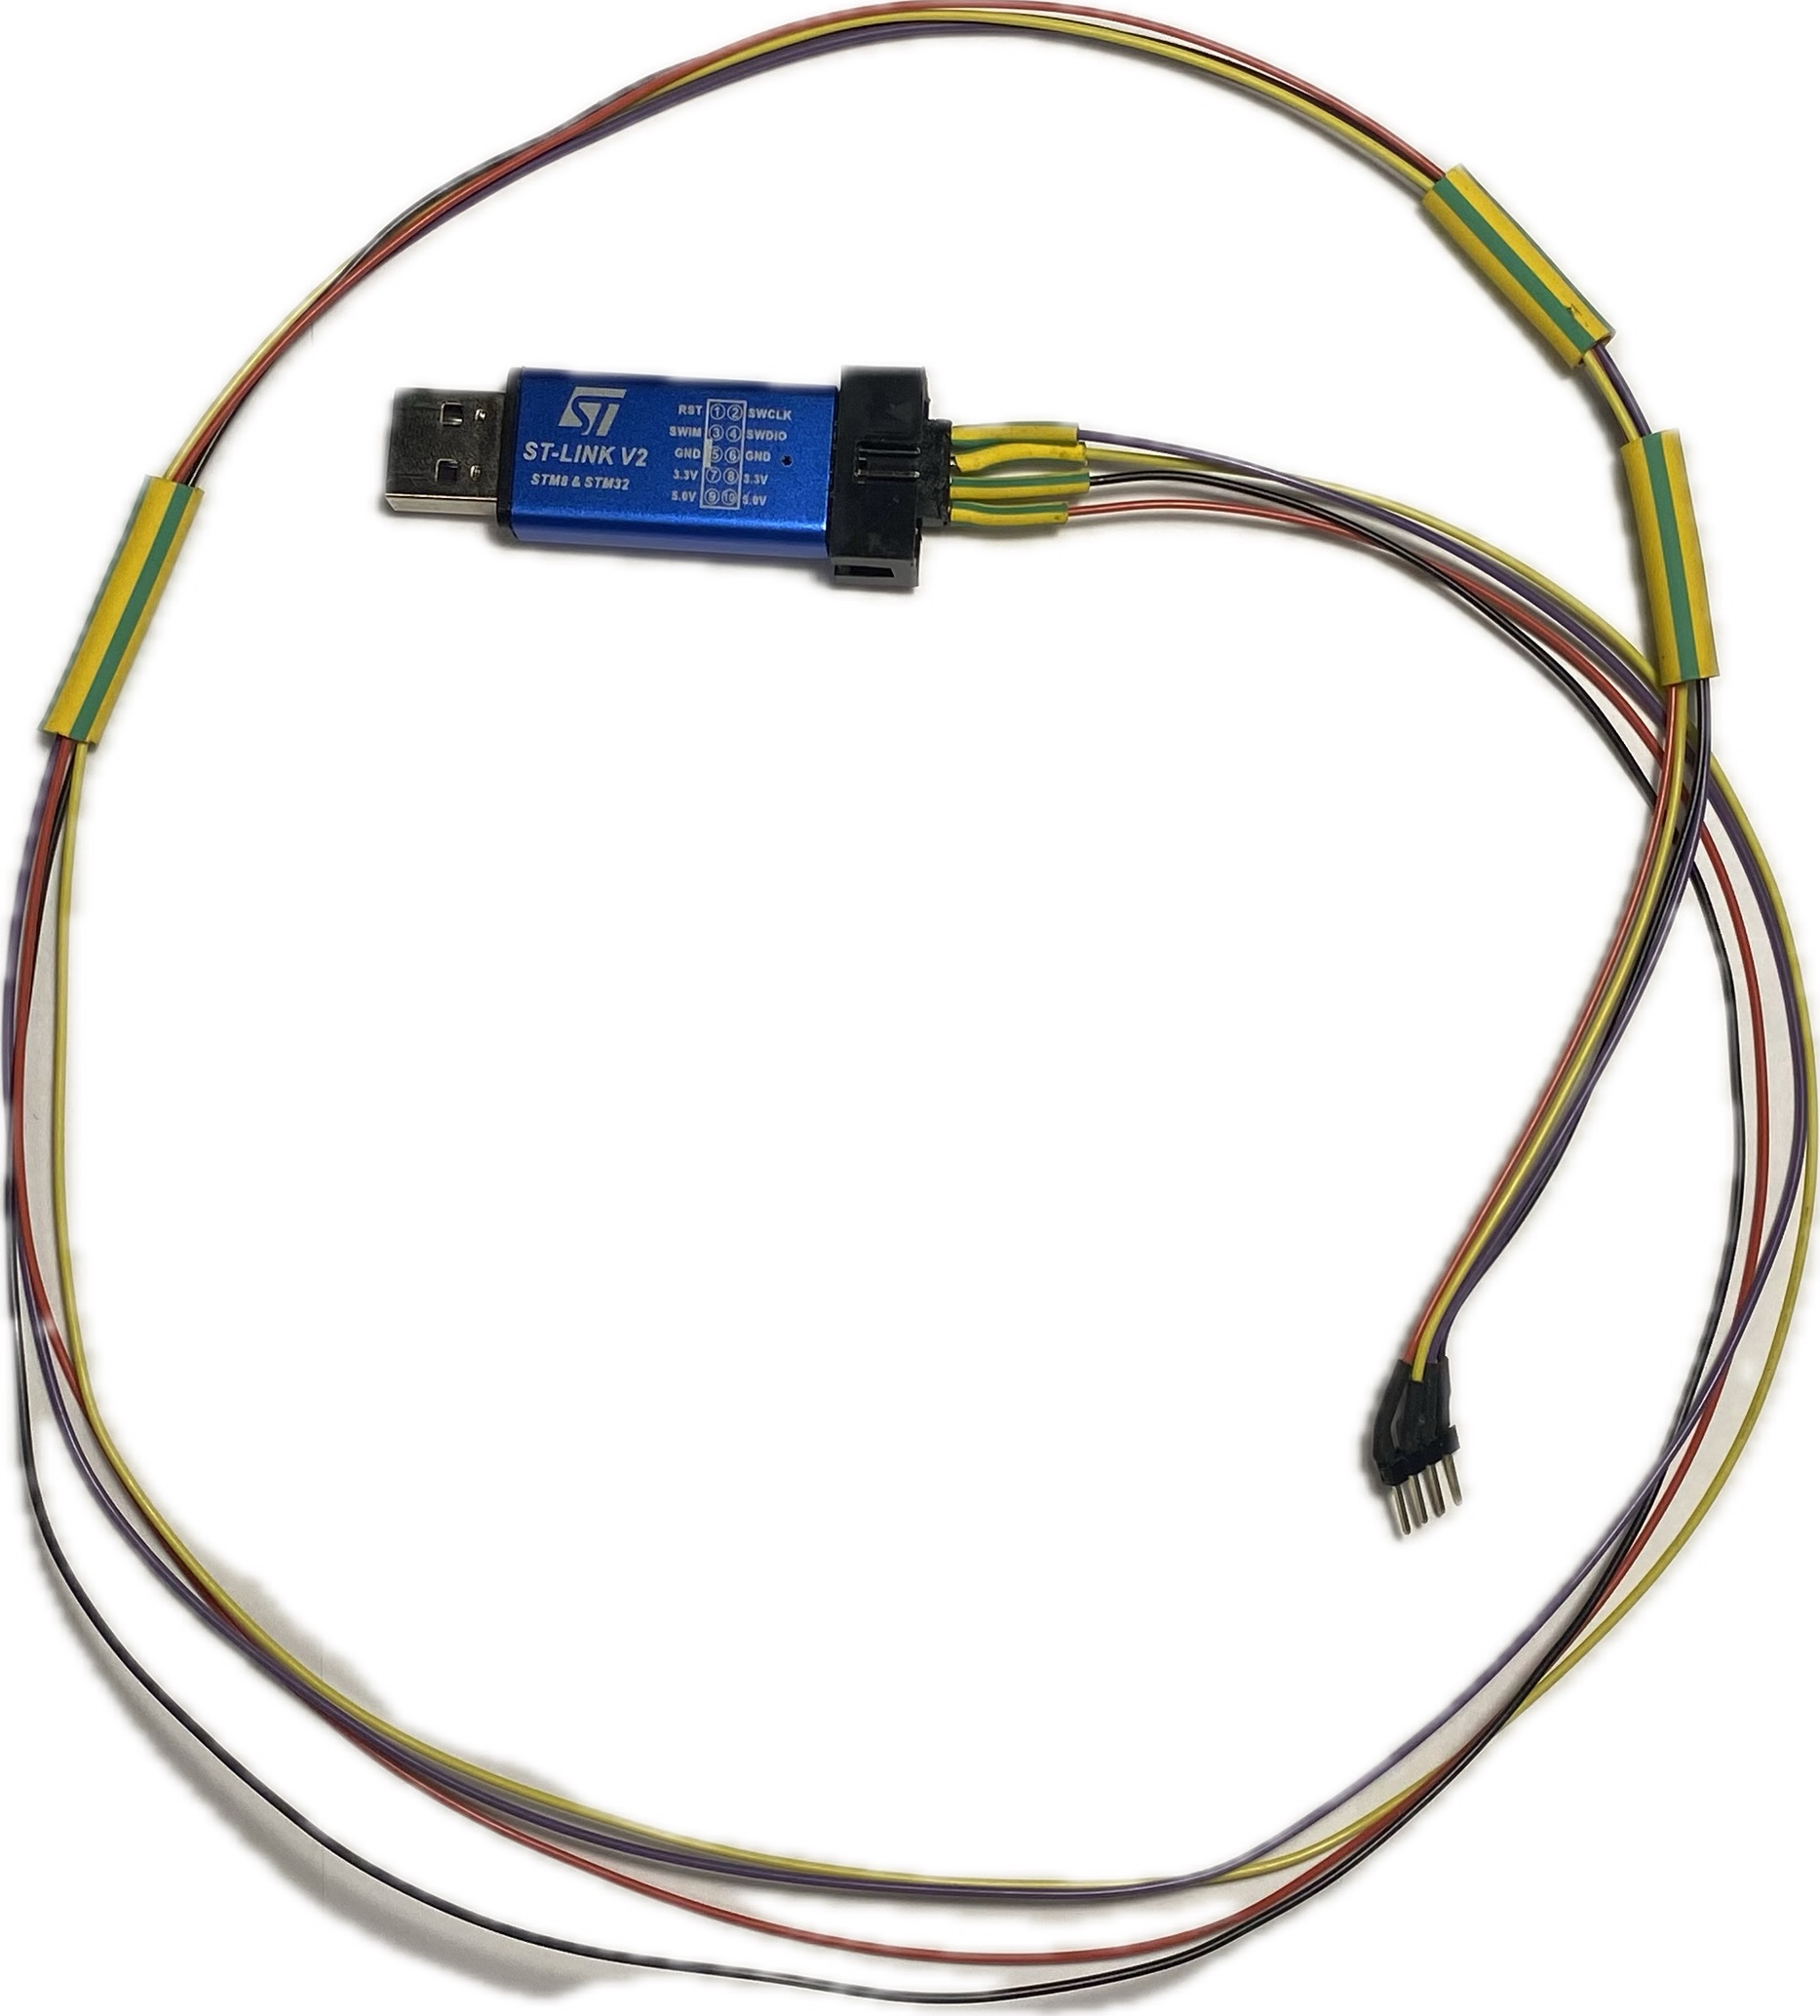
\includegraphics[width=0.45\linewidth]{ST-LINK.jpeg}
    \caption{ST-LINK}
    \label{fig:st-link}
\end{figure}
\newpage
\begin{table}[h]
\begin{threeparttable}
\caption{Power Node (and Analog Node v2.2) Chip\cite{ref8} Characteristics}
\label{table:power_node_char}
\begin{tabularx}{\textwidth}{l c | c| c c c | c | X}
    \thickhline
    \textbf{Parameter} & & \textbf{Symbol} & \textbf{Min.} & \textbf{Typ.} & \textbf{Max.} &
    \textbf{Unit} & \textbf{Conditions} \\
    \hline
    Supply Voltage & &$V_{DD}$ & 1.71 & 3.3 & 3.6 & V \\
    \hline
    External Oscillator Frequency & &$f_{OSC\_IN}$ & 4 & 8 & 48 & MHz \\
    \hline
    Current Consumtion & &$I_{c(MCU)}$ & \textcolor{red}? & \textcolor{red}? & \textcolor{red}? & mA \\
    \hline
    Voltage Input Low I/O & &$V_{IL}$ & - & - & $0.3*V_{DD}$ & V & \multirow{2}{*}{$1.62 V<V_{DD}<3.6 V$}\\
    \cline{1-7}
    Voltage Input High I/O\tnote{1} & &$V_{IH}$ & $0.7*V_{DD}$ & - & - & V & \\
    \hline
    Voltage Output Low I/O\tnote{2} & &$V_{OL}$ & - & - & 1.3 & V & $|I_{IO}| = 20 mA$ \\
    \cline{1-7}
    Voltage Output High I/O\tnote{2} & &$V_{OH}$ & $V_{DD}-1.3$ & - & - & V & $V_{DD} >= 2.7 V$\\
    \hline
    Current Output I/O for 1 pin & &$I_{IO(PIN)}$ & - & - & 20 & mA & \\
    \hline
    Current Output I/O total\tnote{3} & &$I_{IO(SUM)}$ & - & - & 100 & mA & \\
    \hline
    Analog Supply Voltage & &$V_{DDA}$ & 1.62 & - & 3.6 & V & \\
    \hline    
    ADC Voltage Range & &$V_{ADC}$ & $V_{SSA}$\tnote{4} & - & $V_{DDA}$ & V & \\
    \hline
    Total Current through MCU & &$I_{MCU}$ & - & - & 150 & mA & \\
    \hline
    \thickhline
\end{tabularx}
\begin{tablenotes}
\item[1] {Some pins on the chip are tolerant of incoming 5V, but it is strongly recommended to familiarise with the original datasheet of the chip before using this option.}
\item[2] {This specifications applies to most I/O pins and shows absolute values, but more data with different conditions is available in the datasheet of the chip.}
\item[3] {This current consumption must be correctly distributed over all I/Os and control pins.}
\item[4] {Analog Ground}
\end{tablenotes}
\end{threeparttable}
\end{table}
\newpage
\subsubsection{Power Switches}
\label{sssec:power_switch}
In order to realize full control over the vehicle's functions, a system of high-side drivers was implemented. Nodes v1 used a high-side driver, which was not reliable enough for active use, so the new versions used the best component in terms of its characteristics at the time of writing, the VNQ9080AJ\cite{ref11} (\textit{IC1} and \textit{IC2}), which proved to be quite reliable in many use scenarios. But starting from version 2.2.5 it is recommended to use VNQ9025AJ\cite{ref16}, which is almost exactly the same component as before, but has improved characteristics in terms of current and resistance. One such component is capable of providing 4 outputs, so to provide 8 outputs, two such components are used simultaneously, which are controlled using signals from the Power Node chip, which is mentioned in the previous Section \nameref{ssec:power_node}. In general, this is the most important functionality that Power Node can provide, because the functionality and stability of the key parts of the car depend on it, so special attention should be paid when soldering, testing and using this functionality. As shown in Figure \ref{fig:power_switch}, resistors are connected to some of the driver pins. Their values and presence were chosen in strict accordance with the component datasheet and provide some protection against unexpectedly increased currents. \\
\begin{figure}[h]
    \centering
    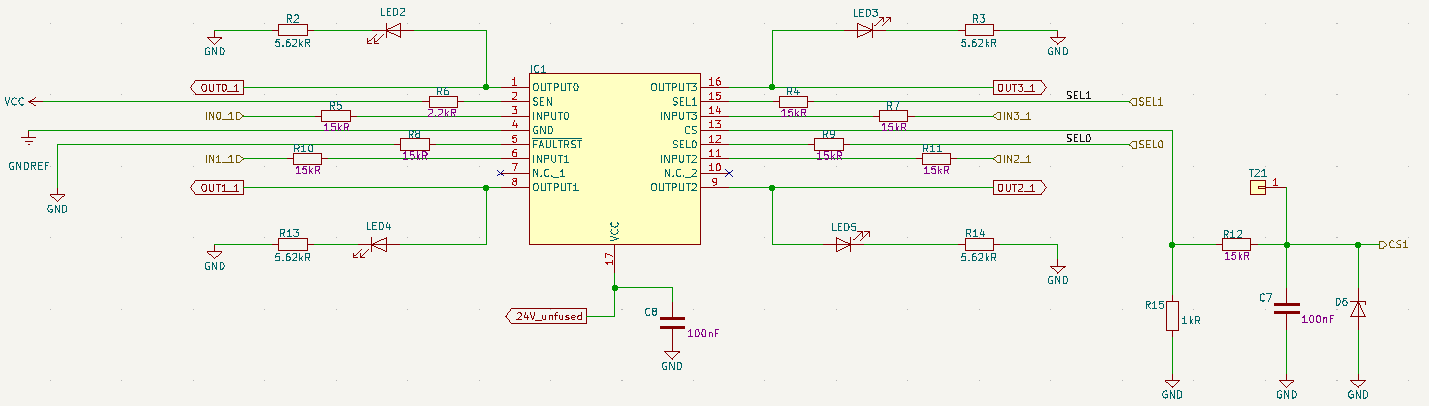
\includegraphics[width=1\linewidth]{Power Switch.png}
    \caption{High-Side Driver Schematic}
    \label{fig:power_switch}
\end{figure}
\begin{table}[h]
\begin{threeparttable}
\caption{High-Side Driver Pin Functions}
\label{table:power_switch_pins}
\begin{tabularx}{\textwidth}{ c | X }
    \thickhline
    \textbf{Name} & \textbf{Function} \\
    \hline
    {$V_{cc}$} & Power connection; The driver itself is connected to 24V, which immediately comes to the board, bypassing the fuse, because the high-side driver itself represents the functionality of the fuse. The fact that the datasheet of this component allows it to be used at higher voltages, as well as its parallel connection on the board, does not give permission to supply higher voltages. The maximum permissible voltage supplied to the board is mentioned in Table \ref{table:elec_char}.  \\
    \hline
    $OUT_{0-3}$ & Power output \\
    \hline
    $GND$ & Ground connection; The ground of this component is isolated in some sense from the rest using diode \textit{D1} and resistor \textit{R30}, as shown in Figure \ref{fig:power_switch_gnd}.\\
    \hline
    $IN_{0-3}$ & Voltage controlled input pin; controls output switch state.\\
    \hline
    $CS$ & Analog current sense output pin; it delivers a current proportional to the selected load current. \\
    \hline
    $SEn$ & Enables the CS diagnostic pin. \\
    \hline
    $SEL_{0,1}$ & Addresses the CS multiplexer. \\
    \hline
    $FaultRST$ & Unlatches the output in case of fault - if kept low, sets the output to auto-restart mode. \\
    \hline
    \thickhline
\end{tabularx}
\begin{tablenotes}
\item[1] {Some pins on the chip are tolerant of incoming 5V, but it is strongly recommended to familiarise with the original datasheet of the chip before using this option.}
\end{tablenotes}
\end{threeparttable}
\end{table}
\newpage
\begin{figure}[H]
    \centering
    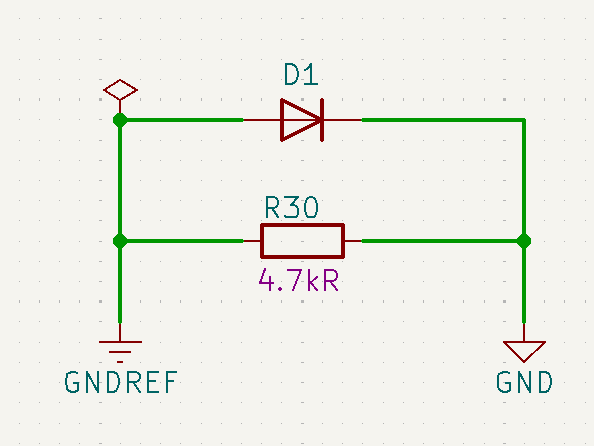
\includegraphics[width=0.22\linewidth]{Power Switch GND.png}
    \caption{Ground Connection for the High-Side Driver}
    \label{fig:power_switch_gnd}
\end{figure}
Each High-Side Driver output has its own LED that shows the power status. And each LED has its own color, so that in the field it is easier to navigate and understand what is responsible for what. More information about this can be found in Section \nameref{ssec:led_code}. \\
This High-Side Driver has a $CS$ pin that sends a current signal proportional to the current at the output of a particular pin, which was selected as a result of interaction with the $SEL0$ and $SEL1$ pins (see Table \ref{table:power_switch_truth_table} for the truth table).
\begin{table}[H]
\begin{threeparttable}
\caption{High-Side Driver Truth Table\tnote{1}}
\label{table:power_switch_truth_table}
\begin{tabularx}{\textwidth}{l | c | c | c c | c | X}
    \thickhline
    \textbf{Mode} & \textbf{$IN_x$} & \textbf{$OUT_x$} & \textbf{$SEL_0$} & \textbf{$SEL_1$} &
    \textbf{$CS$}\tnote{3} & \textbf{Conditions} \\
    \hline
    \multirow{4}{*}{Normal\tnote{2}} & \multirow{2}{*}{L} & \multirow{2}{*}{L} & L & L & $I_{SENSE} = I_{OUT_0}/K$ & \\
    \cline{4-6}
    & & & H & L &$I_{SENSE} = I_{OUT_1}/K$ & Nominal load connected;\\
    %\cline{3-4}
    \cline{4-6}
    & \multirow{2}{*}{H} & \multirow{2}{*}{H} & L & H & $I_{SENSE} = I_{OUT_2}/K$ & $T_j < 150\degree C$\\
    \cline{4-6}
    & & & H & H & $I_{SENSE} = I_{OUT_3}/K$ & \\
    \hline
    \multirow{4}{*}{Overload} & \multirow{2}{*}{L} & \multirow{2}{*}{L} & \multirow{4}{*}{X} & \multirow{4}{*}{X} & \multirow{4}{*}{$V_{SENSE} = V_{SENSEH}$} & Overload or short to GND\\
    & & & & & & causing:\\
    & \multirow{2}{*}{H} & \multirow{2}{*}{H} & & & & $T_j>T_{TSD}$ or \\
    & & & & & & $\Delta T_j>\Delta T_{j\_SD}$\\
    \hline
    Undervoltage & X & L & X & X & Hi-Z & $V_{CC} < V_{USD}$ (falling) \\
    \hline
    OFF-state diagnostics & L & H & X & X & $V_{SENSE} = V_{SENSEH}$ & Short to $V_{cc}$ or Open-load \\
    \hline
    Negative output voltage & L &$<0V$ & X & X & Hi-Z & Inductive loads turn-off \\
    \hline
    \thickhline
\end{tabularx}
\begin{tablenotes}
\item[1] {This table is a shortened version of the component truth table. FaultRST = L and SEn = H for all cases presented in this table, as dictated by the design decisions.}
\item[2] {The $IN_x$ and $OUT_x$ values are not related to the $SEL_x$ and $CS$ values.}
\item[3] {The value of K is mentioned in the Table \ref{table:power_switch_char}}
\end{tablenotes}
\end{threeparttable}
\end{table}
By measuring the current $I_{SENSE}$ on the $CS$ pin, the current on each output pin $I_{OUT}$ can be obtained, where the current value $I_{SENSE}$ is K (from Table \ref{table:power_switch_char}) times less than the current on the output pin $I_{OUT}$. That is, to calculate the output current on the selected pin, the Formula \ref{eq:current_sense} can be used.
\begin{equation}
\label{eq:current_sense}
I_{SENSE} = I_{OUT_{0-3}} / K
\end{equation}
%The value of the $I_{SENSE}$ current on the $CS$ pin will be equal to the current at the dedicated output pin $I_{OUT}$ divided by the K value (approximately 1500), as written in Table \ref{table:power_switch_truth_table} under normal operation ($I_{SENSE} = I_{OUT0-3} / K$). \\ 
But the chip that should read these changes can only measure the voltage $V_{SENSE}$, and not the current $I_{SENSE}$, Formula \ref{eq:voltage_sense} shows the necessary and approximate calculation of Vsense using the product of the resistance $R_{SENSE}$ (\textit{R15} or \textit{R29}) and the current $I_{SENSE}$.
\begin{equation}
\label{eq:voltage_sense}
V_{SENSE} = R_{SENSE} * I_{SENSE}
\end{equation}
%The $V_{SENSE}$ voltage, which will be an indicator for the chip, is equal to the product of the resistor resistance \textit{R15} or \textit{R29} and $I_{SENSE}$ ($V_{SENSE} = R_{SENSE} * I_{SENSE}$). \\ 
But it is strongly recommended to keep in mind the maximum possible voltage on the CS pin $V_{SENSEH}$ under Fault Condition (approximately 7.5V from Table \ref{table:power_switch_char}), since the microchip itself wasn't designed for high values. So it was decided in version 2.2.4 to add a zener diodes \textit{D5} and \textit{D6} to avoid overvoltages above 3.3V. \\
To measure the voltage, the $V_{SENSE}$ chip uses a built-in 12-bit ADC, where each value from zero voltage to 3.3V is divided into 4096 points (from zero to 4095). That is, the calculation of the ADC value is performed according to Formula \ref{eq:adc_value}.
\begin{equation}
\label{eq:adc_value}
ADC_{value} = (V_{SENSE} / 3.3) * 4095
\end{equation}
By combining Formulas \ref{eq:current_sense}, \ref{eq:voltage_sense}, \ref{eq:adc_value}, the current output $I_{OUT}$ on the pin can be calculated based on the measured ADC value by Formula \ref{eq:current_out_adc}.
\begin{equation}
\label{eq:current_out_adc}
I_{OUT_{0-3}} = ADC_{value} * K * 3.3/(R_{SENSE}*4095)
\end{equation}
When connecting any equipment to the outputs, it is worth remembering the total maximum permissible current limit $I_{LIMH}$ supplied to the output pins from Table \ref{table:power_switch_char}. If this value is exceeded, the component will go into protection and turn off as if it had overheated or reached the power limit. So it is necessary to correctly calculate the needs and balance the connection without overloading one component. \\
In case of replacing the High-Side Driver, the values of K and the maximum permissible current limit $I_{LIMH}$ also change as a result, therefore, for a more accurate and safe calculation of the current consumed on the line, it is important to change the resistance of $R_{SENSE}$ according to Formula \ref{eq:res_sense} so that the measurements for the chip continue to be in the range from zero to 3.3V, which means for the current from zero to the maximum permissible value. 
\begin{equation}
\label{eq:res_sense}
R_{SENSE} = 3.3*K/I_{LIMH}
\end{equation}
After this change, it is also necessary to update the code variables, which are the values of K and $R_{SENSE}$, so that the formula continues to calculate the current consumed on the line correctly with the new component. \\
But theoretically it is even possible not to change the code, but just change the resistance of $R_{SENSE}$, since in fact, when the component is changed, the ratio between K and Rsense changes, which affects the calculation of the ADC value, which means that if this ratio is kept constant with the new High-Side Driver can continue to use the same variables in the code as before. By combining this understanding of the constancy of the ratio and Formula \ref{eq:res_sense}, Formula \ref{eq:res_sense_new} can be obtained, where it possible to calculate the appropriate resistance value for this specific case.
\begin{equation}
\label{eq:res_sense_new}
R_{SENSE_{new}}=R_{SENSE_{old}}*K_{new}/K_{old}=3.3*K_{new}/I_{LIMH_{old}}
\end{equation}
But it is important to understand that when increasing the resistance, the $V_{SENSE}$ voltage at maximum current also increases, which means that in the best case, the current values will be lost when calculating above the maximum value that was before, and in the worst case, this action can damage the chip due to increased voltage. And vice versa, when decreasing the resistance, the measurement accuracy decreases significantly, so the action of replacing the component and resistance without changing the variables in the code is not recommended and can be used only in the most extreme cases.
\begin{table}[H]
\begin{threeparttable}
\caption{Selecting and Calculating a Suitable $R_{SENSE}$ Value}
\label{table:power_switch_pins}
\begin{tabularx}{\textwidth}{ c | X }
    \thickhline
    \textbf{$R_{SENSE}$\tnote{1}} & \textbf{Conditions}\\
    \hline
    $R_{SENSE}=3.3*5050/8\approx2083,1\Omega$\tnote{2} & Placement of component VNQ9025AJ\cite{ref16} or replacement of component VNQ9080AJ\cite{ref11} with this one \textbf{with} changing the necessary variables in the code.\\
    \hline
    $R_{SENSE}=3.3*1500/4.2\approx1178.6\Omega$\tnote{2} & Placement of component VNQ9080AJ\cite{ref16} or replacement of component VNQ9025AJ\cite{ref11} with this one \textbf{with} changing the necessary variables in the code.\\
    \hline
    $R_{SENSE}=3.3*5050/4.2\approx3967.9\Omega$\tnote{3} & Replacement of component VNQ9080AJ\cite{ref11} with VNQ9025AJ\cite{ref16} \textbf{without} changing the variables of previous component in the code.\\
    \hline
    $R_{SENSE}=3.3*1500/8\approx618.8\Omega$\tnote{3} & Replacement of component VNQ9025AJ\cite{ref11} with VNQ9080AJ\cite{ref16} \textbf{without} changing the variables of previous component in the code.\\
    \hline
    \thickhline
\end{tabularx}
\begin{tablenotes}
\item[1] {Suitable values for variables are taken from Table \ref{table:power_switch_char}}
\item[2] {According to the Formula \ref{eq:res_sense}}
\item[3] {According to the Formula \ref{eq:res_sense_new}}
\end{tablenotes}
\end{threeparttable}
\end{table}
\newpage
All specifications are for $T_j = 25\degree C$ unless otherwise noted.\\\\
If there is $>$ or $<$ symbol before the number, it means that for the case of $V_{cc}=24V$ the value could be bigger or smaller respectively.
\begin{table}[H]
\begin{threeparttable}
\caption{High-Side Driver Characteristics}
\label{table:power_switch_char}
\begin{tabularx}{\textwidth}{l c | c| c c c | c | X}
    \thickhline
    \textbf{Parameter} & & \textbf{Symbol} & \textbf{Min.} & \textbf{Typ.} & \textbf{Max.} &
    \textbf{Unit} & \textbf{Conditions} \\
    \hline
    Supply Voltage & &$V_{cc}$ & 4 & 24\tnote{1} & 28 & V \\
    \hline
    Undervoltage shutdown & & $V_{USD}$ & - & 2.1 & 2.7 & V & \\
    \hline
    \multicolumn{1}{l|}{\multirow{4}{*}{On-state Resistance}} & \multirow{2}{*}{\cite{ref11}} &\multirow{4}{*}{$R_{ON}$} & \multirow{2}{*}{-} & \multirow{2}{*}{$>86$} & \multirow{2}{*}{-} & \multirow{4}{*}{m$\Omega$} & $I_{OUT} = 0.7A;$\\
    \multicolumn{1}{l|}{} & & & & & & &$V_{cc}=13V$\\
    \cline{2-2}
    \cline{4-6}
    \cline{8-8}
    \multicolumn{1}{l|}{} & \multirow{2}{*}{\cite{ref16}} & & \multirow{2}{*}{-} & \multirow{2}{*}{$>25$} & \multirow{2}{*}{-} & & $I_{OUT} = 2.1A;$ \\
    \multicolumn{1}{l|}{} & & & & & & &$V_{cc}=13V$\\
    \hline 
    \multicolumn{1}{l|}{\multirow{2}{*}{Current Limitation\tnote{2}}} & \cite{ref11} & \multirow{2}{*}{$I_{LIMH}$} & - & $<4.2$ & - & \multirow{2}{*}{A} & \multirow{2}{*}{$V_{cc}=22V$}\\
    \cline{2-2}
    \cline{4-6}
    \multicolumn{1}{l|}{} & \cite{ref16} & & - & $<8$ & - & &\\
    \hline
    \multirow{5}{*}{Current Supply} & &\multirow{5}{*}{$I_S$} & \multirow{5}{*}{-} & \multirow{5}{*}{$>5.5$} & \multirow{5}{*}{7.5} & \multirow{5}{*}{mA} & $V_{cc} = 13V;$\\
    & & & & & & &$V_{SEn} = V_{FR} = $\\
    & & & & & & &$= V_{SEL} = 0V;$\\
    & & & & & & &$V_{IN} = 5V;$\\
    & & & & & & &$I_{OUT} = 0A$\\
    \hline
    Voltage Input Low\tnote{3} & &$V_{INL}$ & - & - & 0.9 & V & \\
    \hline
    Voltage Input High\tnote{3} & &$V_{INH}$ & 2.1 & - & - & V & \\
    \hline
    CS Voltage Output in Fault Condition & & $V_{SENSEH}$ & 5 & - & 7.5 & V & $13V < V_{cc} < 18V$ \\
    \hline
    \multicolumn{1}{l|}{\multirow{6}{*}{Ratio K ($I_{OUT}/I_{SENSE}$)}} & \multirow{3}{*}{\cite{ref11}} & \multirow{6}{*}{$K$} & \multirow{3}{*}{-5\%} & \multirow{3}{*}{1500} & \multirow{3}{*}{5\%} & & $I_{OUT}= 2.1A;$\\
    \multicolumn{1}{l|}{} & & & & & & &$V_{SENSE} = 3.5V;$\\
    \multicolumn{1}{l|}{} & & & & & & &$V_{SEn} = 5V$\\
    \cline{2-2}
    \cline{4-6}
    \cline{8-8}
    \multicolumn{1}{l|}{} & \multirow{3}{*}{\cite{ref16}} & & \multirow{3}{*}{-5\%} & \multirow{3}{*}{5050} & \multirow{3}{*}{5\%} & & $I_{OUT}= 6.3A;$\\
    \multicolumn{1}{l|}{} & & & & & & &$V_{SENSE} = 3.5V;$\\
    \multicolumn{1}{l|}{} & & & & & & &$V_{SEn} = 5V$\\
    \hline
    Shutdown temperature & & $T_{TSD}$ & 150 & 175 & 210 & $\degree$C & \\
    \hline
    Dynamic temperature & & $\Delta T_{j\_SD}$ & - & $<55$ & - & $\degree$C & $V_{cc} = 19V$\\
    \hline
    \thickhline
\end{tabularx}
\begin{tablenotes}
\item[1] {This number is not dictated by the datasheet, but by the use of the component in Nodes itself. In the datasheet, a typical number is 13V.}
\item[2] {$I_{LIMH}=MAX(I_{OUT})$}
\item[3] {This is also true for the SEL and SEn pins.}
\end{tablenotes}
\end{threeparttable}
\end{table}
\newpage
\subsubsection{PWM}
\label{sssec:pwm}
In order to control the power of connected equipment, such as fans or pumps, using a digital signal, the Nodes have a PWM (Pulse-width modulation) function implemented on two pins, which, as a result of changing the duty cycle, affects the operation of the equipment using just one connected signal. The larger the duty cycle, the greater the power consumption (for example, a fan rotates faster with a larger duty cycle). It is also important to comply with the permissible PWM signal frequencies for connected devices, which can be found in their datasheets.
\\ Some devices require a PWM signal of greater amplitude, while the chip on the Power Node can only output 3.3V amplitude of the required signal. Therefore, starting with version 2.2.2, Level-Shifters are actively used as shown in Figure \ref{fig:pwm_level}. The way the Level Shifter works in this setup can be confusing, but there is an explanation for its functionality. Due to the lack of ground in this circuit, the supplied low signal pulls the current from the high voltage to itself and as a result, almost zero is formed on the output signal, because the current chooses the path of least resistance to the ground, and since Level-Shifter consists of a MOSFET transistor TN2106\cite{ref13} (\textit{Q1} and \textit{Q2}), it does not pass through itself a voltage higher than 3.3V, since this voltage is connected to the gate. If the input signal is high, then the current of higher voltage does not go towards the transistor, because now the path is closed for it and as a result, a high signal of increased amplitude is formed at the output.
\begin{figure} [h]
    \centering
    
\includegraphics[width=0.85\linewidth]{Datasheet_electronics/PWM.png}
    \caption{PWM Waveforms\cite{ref12}}
    \label{fig:pwm_wave}
\end{figure}
\\ Starting with version 2.2.3, both pins are capable of providing an increased controlled amplitude, while 2.2.2 can only provide 24V on one PWM1. In version 2.2.3, it became possible to change the amplitude of the output signal as needed using a small switch and easily select one of three modes (3.3V, 5V and 24V), which provides greater versatility and ease of use and testing.
\begin{figure} [h]
    \centering
    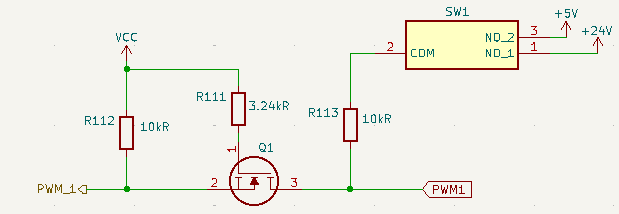
\includegraphics[width=0.85\linewidth]{PWM_Level-Shifter.png}
    \caption{PWM Level-Shifter}
    \label{fig:pwm_level}
\end{figure}
\newpage
\subsection{Analog Node}
\label{ssec:analog_node}
Another equally important part of Nodes is the Analog Node. The Analog Node chip acts as a processor of filtered signals received from connected sensors, and then sends the received data further via CAN.
The Analog Node power is supplied separately from the main 3.3V power supply to ensure maximum stability and safety of this part, which is critical for the analog signal processing. The Analog Node power is controlled using the Power Node, as described in Section \nameref{sssec:control_power}. In version 2.1, the controlled power is supplied from the switch, and in version 2.2, it is supplied from the voltage regulator. \\
Both versions have 16 ADC inputs with different amplitudes (3.3V; 5V and 24V) that can handle incoming analog signals (more information about this in Section \nameref{sssec:filters}), as well as three I2C inputs that can accept digital signals from connected sensors, which increases the versatility of the board and allows for a wider range of use cases. \\
There are also two controllable LEDs (\textit{LED10} and \textit{LED11}) that can be used to monitor the operation of the chip and certain functions. More information about the LEDs can be found in Section \nameref{ssec:led_code}. \\
This section contains information that differs from the information described earlier, so first of all it is worth looking at Section \nameref{ssec:power_node}, which also describes the basic operating principles of the STMicroelectronics chip and the nuances associated with it, such as JTAG, BOOT pin and others.
\subsubsection{Analog Node v2.1}
The Analog Node version 2.1 uses the STM32H7B0RBT6\cite{ref14} (\textit{U2}) chip, which has two CANs, but only one of them was actively used. Unfortunately, the chip did not show its best side in practical use, namely insufficient reliability and price.
\\ This version makes active use of the external ASE-25.000MHZ-LC-T\cite{ref15} (\textit{Y2}) oscillator, which provides a stable and recommended frequency of 25 MHz according to the Table \ref{table:analog_node_char}.\\
\begin{figure} [h]
    \centering
    
\includegraphics[width=1\linewidth]{Datasheet_electronics/Analog_Node_v21.png}
    \caption{Analog Node schematic v2.1}
    \label{fig:analog_node_v21}
\end{figure}
\begin{table} [H]
\begin{threeparttable}
\caption{Analog Node v2.1 Chip\cite{ref14} Characteristics}
\label{table:analog_node_char}
\begin{tabularx}{\textwidth}{l c | c| c c c | c | X}
    \thickhline
    \textbf{Parameter} & & \textbf{Symbol} & \textbf{Min.} & \textbf{Typ.} & \textbf{Max.} &
    \textbf{Unit} & \textbf{Conditions} \\
    \hline
    Supply Voltage & &$V_{DD}$ & 1.62 & 3.3 & 3.6 & V \\
    \hline
    External Oscillator Frequency & &$f_{OSC\_IN}$ & 4 & 25 & 50 & MHz \\
    \hline
    Current Consumtion & &$I_{c(MCU)}$ & \textcolor{red}? & \textcolor{red}? & \textcolor{red}? & mA \\
    \hline
    Voltage Input Low I/O & &$V_{IL}$ & - & - & $0.3*V_{DD}$ & V & \multirow{2}{*}{$1.62 V<V_{DD}<3.6 V$}\\
    \cline{1-7}
    Voltage Input High I/O\tnote{1} & &$V_{IH}$ & $0.7*V_{DD}$ & - & - & V & \\
    \hline
    Voltage Output Low I/O\tnote{2} & &$V_{OL}$ & - & - & 1.3 & V & $|I_{IO}| = 20 mA$ \\
    \cline{1-7}
    Voltage Output High I/O\tnote{2} & &$V_{OH}$ & $V_{DD}-1.3$ & - & - & V & $V_{DD} >= 2.7 V$\\
    \hline
    Current Output I/O for 1 pin & &$I_{IO(PIN)}$ & - & - & 20 & mA & \\
    \hline
    Current Output I/O total\tnote{3} & &$I_{IO(SUM)}$ & - & - & 140 & mA & \\
    \hline
    Analog Supply Voltage & &$V_{DDA}$ & 1.62 & - & 3.6 & V & \\
    \hline    
    ADC Voltage Range & &$V_{ADC}$ & $V_{SSA}$\tnote{4} & - & $V_{DDA}$ & V & \\
    \hline
    Total Current through MCU & &$I_{MCU}$ & - & - & 620 & mA & \\
    \hline
    \thickhline
\end{tabularx}
\begin{tablenotes}
\item[1] {Some pins on the chip are tolerant of incoming 5V, but it is strongly recommended to familiarise with the original datasheet of the chip before using this option.}
\item[2] {This specifications applies to most I/O pins and shows absolute values, but more data with different conditions is available in the datasheet of the chip.}
\item[3] {This current consumption must be correctly distributed over all I/Os and control pins.}
\item[4] {Analog Ground}
\end{tablenotes}
\end{threeparttable}
\end{table}
\newpage
\subsubsection{Analog Node v2.2}
In this version, Analog Node has acquired a new chip STM32G431RBT6\cite{ref8} (\textit{U11}) of the same group as the chip from Power Node, which required code adaptation, but allowed using a cheaper, more reliable and time-tested chip compared to what was before. Also, as a result of changing the chip, only one CAN line remained, which optimized and simplified the board in use. The oscillator is now exactly the same as on Power Node and produces 8 MHz, which is still sufficient. In general, this is the same chip as for Power Node, but the selected chip has a larger number of pins and more possible connections. More information about the chip can be found in Section \nameref{ssec:power_node}.
\begin{figure} [h]
    \centering
    
\includegraphics[width=1\linewidth]{Datasheet_electronics/Analog_Node_v22.png}
    \caption{Analog Node schematic v2.2}
    \label{fig:analog_node_v22}
\end{figure}
\newpage
\subsubsection{Filters}
\label{sssec:filters}
Filters are a very important part of Analog Node, because vital signals from sensors pass through them to have more stable and readable data. The filtering system consists of several important elements, namely an active low-pass filter, consisting of a simple and understandable op-amp LM358\cite{ref17}, which is intelligently combined with a passive low-pass filter, consisting of RLC components, which ensures maximum versatility and quality of signal filtering, and a voltage divider, which in combination with a capacitor also forms a low-pass filter. This system both filters the signal actively and passively, and also reduces the signal amplitude to readable for the chip 3.3V, and it is absolutely unique in its simplicity and ease of use, as well as the quality provided, so as a result of which, starting from the Nodes old version v1, the design remains unchanged to this day. \\ 
In total, there are 16 possible connections, but two of them are allocated for a signal with an amplitude of 3.3V (Figure \ref{fig:filter_3v3}), seven filters for 5V (Figure \ref{fig:filter_5v}), three filters for a signal with an amplitude of 24V (Figure \ref{fig:filter_24v}) and the remaining 4 are allocated for the future for the idea of conveniently connecting additional filters, which is still at the concept stage, so it can be removed in the future. \\
If for some reason the sensors produce a non-standard signal amplitude, which was not initially included in the Nodes, then the resistance on the voltage divider needs to be recalculated with Formula \ref{eq:voltage_filter}, where $R_L$ is resistor connected to the ground (for example \textit{R99} from the Figure \ref{fig:filter_5v}) and $R_H$ connected to the filter (for example \textit{R96} from the Figure \ref{fig:filter_5v}).
\begin{equation}
\label{eq:voltage_filter}
V_{OUT}=V_{IN}*R_L/(R_L+R_H)
\end{equation}
Formula \ref{eq:voltage_filter} could be simplified into Formula , because $R_L$ = $3.24k\Omega$ and $V_{OUT} = 3.3V$ in most cases.
\begin{equation}
R_H=3.24*10^3*(V_{IN}/3.3-1)
\end{equation}
The supplied voltage should not be higher than the powered voltage, namely 24V, to avoid breakdowns and problems with op-amp. 
\\ Each output has a testpoint (for example \textit{T20}) that can be used for testing, but more information about this can be found in Section \nameref{ssec:testpoint}. 
\\ If the supplied signal amplitude is greater than 9V, then it is necessary to use a 1nF capacitance instead of 10nF capacitors like on the Figure \ref{fig:filter_24v}. \\Also, if an NTC sensor is connected, it is important to short the inductor (for example \textit{L25} from the Figure \ref{fig:filter_5v}) and the resistor (for example \textit{R95} from the Figure \ref{fig:filter_5v}) on its path, and solder a 680 ohm resistor (for example \textit{R98} from the Figure \ref{fig:filter_5v}) into the DNA position, but this action requires subsequent tests after that. \\When a 5000 step resolution is wanted and lower offset voltage, then it is recommended to use ADA4522-2 or more expensive solutions of the same footprint SOIC-8 instead of LM358\cite{ref17}. \\\\More theoretical information about the operation of filters can be found in the excellent Scott's thesis\cite{ref18} \\
\newpage
\begin{figure} [H]
    \centering
    
\includegraphics[width=0.9\linewidth]{Datasheet_electronics/Filter_3V3.png}
    \caption{Filtering System for 3.3V amplitude signal}
    \label{fig:filter_3v3}
\end{figure}
\begin{figure} [H]
    \centering
    
\includegraphics[width=0.95\linewidth]{Datasheet_electronics/Filter_5V.png}
    \caption{Filtering System for 5V amplitude signal}
    \label{fig:filter_5v}
\end{figure}
\begin{figure} [H]
    \centering
    
\includegraphics[width=0.9\linewidth]{Datasheet_electronics/Filter_24V.png}
    \caption{Filtering System for 24V amplitude signal}
    \label{fig:filter_24v}
\end{figure}
\newpage
\subsection{CAN}
\label{ssec:can}
In order for the communication between Nodes and ECU to be as stable as possible, CAN is used, which, thanks to two connection lines (High and Low), is able to work in a variety of conditions, which is important during active operation of the car. This protocol is quite reliable, simple thanks to the priority system and protected from external interference. In version 2.1, Nodes had two different CANs, but in the new versions 2.2 there is only one left, since the Analog Node chip was replaced. The chips themselves that transmit and receive data are not able to directly send data to the main CAN line, so auxiliary components TCAN1462VDRQ1\cite{ref19} (\textit{IC3} and \textit{IC4}) are used that were specially designed for this. These components are powered by 5V, so if ST-LINK is connected, but not the main 24V power supply, CAN will not work due to insufficient voltage. \\ 
In order for data to be exchanged on the main line, a terminating resistance is needed between High and Low. There must be two terminators at different ends of the main data transmission line and one of them is located on Nodes. The resistance value should be about 120 Ohms on one terminator. In new versions, a switch \textit{SW3} was introduced that allows to connect or disconnect the terminator without soldering, which saves time. In general, just two 60 Ohm resistors connected in series are enough, as it was before, but in new versions, together with the switch, there are now 4 resistors (\textit{R46}, \textit{R37}, \textit{R47} and \textit{R109}) instead of two. This is necessary in case of switching off the terminator, data transmission will not be affected, so it simply bypasses these resistors along the least resistance path.
\begin{figure} [h]
    \centering
    
\includegraphics[width=1\linewidth]{Datasheet_electronics/CAN_Power_Node.png}
    \caption{CAN schematic for Power Node}
    \label{fig:can_power_node}
\end{figure}
\begin{figure} [h]
    \centering
    
\includegraphics[width=1\linewidth]{Datasheet_electronics/CAN_Analog_Node.png}
    \caption{CAN schematic for Analog Node}
    \label{fig:can_power_node}
\end{figure}
\newpage
\section{Electrical Specifications}
\label{sec:elec_spec}
At the time of writing, this section contains mostly theoretical data that was obtained based on the documentation of the components used on the board.
\\\\ All specifications are in $10\degree C \leq T_j \leq 50\degree C$ unless otherwise noted.
\begin{table}[h]
\begin{threeparttable}
\caption{Electrical Characteristics}
\label{table:elec_char}
\begin{tabularx}{\textwidth}{l c | c| c c c | c | X}
    \thickhline
    \textbf{Parameter} & & \textbf{Symbol} & \textbf{Min.} & \textbf{Typ.} & \textbf{Max.} &
    \textbf{Unit} & \textbf{Conditions} \\
    \hline
    \multicolumn{1}{l|}{\multirow{2}{*}{Forward Voltage \textit{D2}\tnote{1}}} & v2.1 &\multirow{2}{*}{$V_{f}$} & - & 500\tnote{\cite{ref2}} & - & \multirow{2}{*}{mV} %& \multirow{2}{*}{Standard A4 paper} 
    \\
    \cline{2-2}
    \cline{4-6}
    \multicolumn{1}{l|}{} & v2.2 & & - & 370\tnote{\cite{ref3}} & - & &
    \\
    \hline
    Voltage Input\tnote{2}  & &$V_{in}$ & 22.8$+V_f$ & 24.0$+V_f$ & 25.2$+V_f$ & V %& \multirow{2}{*}{Standard A4 paper} 
    \\
    \hline
    \multicolumn{1}{l|}{\multirow{2}{*}{Current Consumption}} & v2.1 &\multirow{2}{*}{$I_c$} & \textcolor{red}? & \textcolor{red}? & \textcolor{red}? & \multirow{2}{*}{mA} & \multirow{2}{*}{}\\
    \cline{2-2}
    \cline{4-6}
    \multicolumn{1}{l|}{} & v2.2 & &\textcolor{red}? & \textcolor{red}? &\textcolor{red}? & &
    \\
    \hline
    \multicolumn{1}{l|}{\multirow{4}{*}{Current Output\tnote{3}}} & \multirow{2}{*}{v2.1} &\multirow{4}{*}{$I_o$\tnote{4}} & - & 350$-I_c$ & - & \multirow{4}{*}{mA} & $V_o=3.3V$\tnote{\cite{ref4}}\\
    \cline{4-6}
    \cline{8-8}
    \multicolumn{1}{l|}{}& & & - & 350$-I_c$ & - & &$V_o=5V$\tnote{\cite{ref4}}
    \\
    \cline{2-2}
    \cline{4-6}
    \cline{8-8}
    \multicolumn{1}{l|}{}& \multirow{2}{*}{v2.2} & & - & 300$-I_c$ & - & & $V_o=3.3V$\tnote{\cite{ref5}}
    \\
    \cline{4-6}
    \cline{8-8}
    \multicolumn{1}{l|}{}& & & - & 1000$-I_{o_{3v3}}-I_c$\tnote{5}& - & & $V_o=5V$\tnote{\cite{ref6}}
    \\
    \hline
    \thickhline
\end{tabularx}
\begin{tablenotes}
\item[1] {$V_f$ is the standard forward voltage of the diode \textit{D2} connected in series. So if just 24V are connected to the Nodes it means that the board itself after diode (\textit{D2}) will receive $24-V_f$, which is not critical in theory, but still should be taken into account.}
\item[2]{Based on the datasheet of Zener Diode (\textit{D3})\cite{ref1}.}
\item[3]{The values in this section of the table represent the theoretical maximum current output that a particular output voltage pin can provide on different versions. The values are based on voltage regulators' datasheets, so if your use case requires higher current, it is highly recommended to familiarise with the limitations and assumptions of the voltage regulator on a particular line.} 
\item[4]{In order to at least roughly understand the available current on the line, due to the current consumption of the board itself, it is necessary to calculate available current for the equipment by using presented equation. This calculation does not provide the most accurate value of the output current, since the $I_c$ is the sum of all consumed currents on the board itself (use the maximum value for the calculation from the table for each version or measure by yourself current consumption of the board before an active usage); accordingly, the calculation takes place with a small margin for the board itself.}
\item[5]{To perform this calculation, It is needed to know the output current $I_{o_{3v3}}$ on the line 3.3V, since the 5 volt and 3.3 volt voltage regulators are connected in series in version 2.2, which may affect the current output value, so this fact must be taken into account when connecting additional equipment.}
\end{tablenotes}
\end{threeparttable}
\end{table}
\newpage
\section{Absolute Maximum Ratings}
This section could be updated later, when the team will have more spare boards to test.
\begin{table}[h]
\begin{threeparttable}
\caption{Absolute Maximum Ratings}
\begin{tabularx}{\textwidth}{l | c | c | c | c X}
    \thickhline
    \multirow{2}{*}{\textbf{Parameter}} & \multirow{2}{*}{\textbf{Symbol}} & \multicolumn{2}{c|}{\textbf{Rating}} & \multirow{2}{*}{\textbf{Unit}}  %\hspace{1cm} 
    \\
    \cline{3-4}
    & &v2.1 &v2.2 &
    \\
    \hline
    Maximum allowed current consumption & $I_{max}$ & \multicolumn{2}{c|}{1\tnote{1}} & A\\
    \hline
    %\multirow{2}{*}
    {Maximum repetitive peak reverse voltage} & $V_{RRM}$ & 25\tnote{\cite{ref2}} & 30\tnote{\cite{ref3}} & V \\
    \thickhline
\end{tabularx}
\begin{tablenotes}
\item[1]{This value is dictated by the choice of the fuse. Since the board itself has a connection for the most popular type of fuses, namely blade fuses, the minimum value that is on the market is 1A, but it is strongly recommended to use 0.5A fuses if they will be available to buy, since in many current consumption tests Nodes did not show too high values.}
%\item[2]{Never actually tested, based on the datasheet of the diode \textit{D2}\cite{ref2}.\\\note{Nodes v2.2} \textit{D2} is SX33L\_R1\_00001\cite{ref3}, which has higher $V_{RRM}$ 30V.}
\end{tablenotes}
\end{threeparttable}
\end{table}

\textbf{Note:} Stresses above those listed under Absolute Maximum Ratings can
cause permanent damage to the device. This is a stress rating only. The functional
operation of the device is not implied in any conditions above those indicated
in the Electrical Specifications section.
\newpage
\section{Pin Functions}
\begin{table}[h]
\begin{threeparttable}
\caption{Nodes Pin Functions}
\label{table:nodes_pins}
\begin{tabularx}{\textwidth}{ c | X }
    \thickhline
    \textbf{Name} & \textbf{Function} \\
    \hline
    $+3V3$ & Voltage outputs 3.3V obtained from voltage regulator.\tnote{1}  \\
    \hline
    $+5V$ & Voltage outputs 5V obtained from voltage regulator.\tnote{1} \\
    \hline
    $+24V$ & Voltage outputs 24V after fuse and zener diode.\tnote{1} \\
    \hline
    $PWR_{0-3}$ & Voltage outputs after an additionally connected filter.\tnote{2} \\
    \hline
    $+24V_{IN}$ & Power supply 24V for Nodes.\tnote{1}\\
    \hline
    $GND$ & Ground connection.\\
    \hline
    $AnIN3V3_{0-1}$ & Analog inputs for 3.3V signal amplitude.\tnote{2}\\
    \hline
    $AnIN5V_{0-6}$ & Analog inputs for 5V signal amplitude.\tnote{2} \\
    \hline
    $AnIN24V_{0-2}$ & Analog inputs for 24V signal amplitude.\tnote{2} \\
    \hline
    $AnIN_{0-3}$ & Analog inputs for additionally connected filter.\tnote{2}\\
    \hline
    $PWM_{1-2}$ & PWM outputs with different signal amplitudes.\tnote{3} \\
    \hline
    $OUT0-3_{1-2}$ & Controllable High-Side Driver outputs 24V.\tnote{4} \\
    \hline
    $I2C(1-3)_{SCL-SDA}$ & Input for digital signals of the I2C protocol.\tnote{5} \\
    \hline
    $CANHI$ and $CANLO$ & Connection for CAN. In version 2.1 there are two CANs, but CAN2HI and CAN2LO are the main ones, like in version 2.2, since on this line there is a connection for both Power Node and Analog Node, while CAN1HI and CAN1LO have a connection only for Analog Node.\tnote{6} \\
    \hline
    \thickhline
\end{tabularx}
\begin{tablenotes}
\item[1] {More information in the Sections \nameref{sec:elec_spec} and \nameref{ssec:power}.}
\item[2] {More information in the Section \nameref{sssec:filters}.}
\item[3] {More information in the Section \nameref{sssec:pwm}.}
\item[4] {More information in the Section \nameref{sssec:power_switch}.}
\item[5] {More information in the Section \nameref{ssec:analog_node}.}
\item[6] {More information in the Section \nameref{ssec:can}.}
\end{tablenotes}
\end{threeparttable}
\end{table}
\newpage
\section{LED Colour Description}
This section lists the LEDs on the board and their functions. This may not match the board in practice, as other LEDs may be soldered, so it is recommended to double-check which colors and LEDs are actually on the board before testing and usage.
\label{ssec:led_code}
\begin{table}[H]
\begin{threeparttable}
\caption{LED Description}
\label{table:led}
\begin{tabularx}{\textwidth}{ c | c | X }
    \thickhline
    \textbf{Reference} & \textbf{Colour} & \textbf{Description} \\
    \hline
    $LED1$ & Yellow & Power Node Controlled LED\tnote{1}  \\
    \hline
    $LED2$ & Red & High-Side Driver's LED connected to OUT0\_1\tnote{2} \\
    \hline
    $LED3$ & White & High-Side Driver's LED connected to OUT3\_1\tnote{2} \\
    \hline
    $LED4$ & White & High-Side Driver's LED connected to OUT1\_1\tnote{2} \\
    \hline
    $LED5$ & Red & High-Side Driver's LED connected to OUT2\_1\tnote{2}\\
    \hline
    $LED6$ & Red & High-Side Driver's LED connected to OUT0\_2\tnote{2}\\
    \hline
    $LED7$ & White & High-Side Driver's LED connected to OUT3\_2\tnote{2}\\
    \hline
    $LED8$ & White & High-Side Driver's LED connected to OUT1\_2\tnote{2} \\
    \hline
    $LED9$ & Red & High-Side Driver's LED connected to OUT2\_2\tnote{2} \\
    \hline
    $LED10$ & Green & 1st Analog Node Controlled LED\tnote{3}\\
    \hline
    $LED11$ & Orange & 2nd Analog Node Controlled LED\tnote{3} \\
    \hline
    $LED12$ & Red & +24V\tnote{4} \\
    \hline
    $LED13$ & Yellow & +3.3V\tnote{4} \\
    \hline
    $LED14$ & Green & +5V\tnote{4} \\
    \hline
    $LED15$ & Blue & +3.3V for Analog Node\tnote{5}\\
    \hline
    \thickhline
\end{tabularx}
\begin{tablenotes}
\item[1] {More information in the Section \nameref{ssec:power_node}.}
\item[2] {More information in the Section \nameref{sssec:power_switch}.}
\item[3] {More information in the Section \nameref{ssec:analog_node}.}
\item[4] {More information in the Section \nameref{ssec:power}.}
\item[5] {More information in the Section \nameref{ssec:analog_node}.}
\item[6] {More information in the Section \nameref{sssec:control_power}.}
\end{tablenotes}
\end{threeparttable}
\end{table}
\newpage
\section{Testpoints Description}
\label{ssec:testpoint}
Testpoints allow to measure voltage in a variety of places and check the board’s functionality. In most cases, to measure voltage on Nodes it is necessary to connect the negative probe to T6, which is the ground connection, and the positive probe to any other testpoint to measure the voltage at it. Table 11 lists all testpoints.
\begin{table}[H]
\begin{threeparttable}
\caption{Testpoints Description}
\label{table:testpoint_list}
\begin{tabularx}{\textwidth}{ c | X }
    \thickhline
    \textbf{Reference} & \textbf{Description} \\
    \hline
    $T1$ & The testpoint is used to measure voltage on the analog power supply pin $VDDA$ of Power Node.\tnote{1}  \\
    \hline
    $T2$ & The testpoint is used to measure voltage on the analog power supply pin $VDDA$ of Analog Node.\tnote{2} \\
    \hline
    $T3$ & The testpoint is used to measure voltage across the resistor $R33$ together with the test point $T4$ to find the current consumption of Nodes.\tnote{3} \\
    \hline
    $T4$ & The testpoint is used to measure 24V and also, together with $T3$, to measure current.\tnote{3} \\
    \hline
    $T5$ & The testpoint is used to measure the voltage on the 3.3V power supply line.\tnote{3}\\
    \hline
    $T6$ & Ground testpoint.\\
    \hline
    $T7$ & The testpoint is used to measure the voltage on the 5V power supply line.\tnote{3}\\
    \hline
    $T8$ & The testpoint is used to measure the voltage on the 3.3V power supply line for Analog Node and also, together with $T23$, to measure current on this line.\tnote{4} \\
    \hline
    $T9$ & The testpoint is used to measure the filtered signal on the Analog Input for 24V $\#1$.\tnote{5}\\
    \hline
    $T10$ & The testpoint is used to measure the filtered signal on the Analog Input for 24V $\#2$.\tnote{5}\\
    \hline
    $T11$ & The testpoint is used to measure the filtered signal on the Analog Input for 24V $\#0$.\tnote{5} \\
    \hline
    $T12$ & The testpoint is used to measure the filtered signal on the Analog Input for 5V $\#0$.\tnote{5} \\
    \hline
    $T13$ & The testpoint is used to measure the filtered signal on the Analog Input for 5V $\#1$.\tnote{5} \\
    \hline
    $T14$ & The testpoint is used to measure the filtered signal on the Analog Input for 5V $\#2$.\tnote{5} \\
    \hline
    $T15$ & The testpoint is used to measure the filtered signal on the Analog Input for 5V $\#3$.\tnote{5} \\
    \hline
    $T16$ & The testpoint is used to measure the filtered signal on the Analog Input for 5V $\#4$.\tnote{5} \\
    \hline
    $T17$ & The testpoint is used to measure the filtered signal on the Analog Input for 5V $\#5$.\tnote{5} \\
    \hline
    $T18$ & The testpoint is used to measure the filtered signal on the Analog Input for 5V $\#6$.\tnote{5} \\
    \hline
    $T19$ & The testpoint is used to measure the filtered signal on the Analog Input for 3.3V $\#1$.\tnote{5} \\
    \hline
    $T20$ & The testpoint is used to measure the filtered signal on the Analog Input for 3.3V $\#0$.\tnote{5} \\
    \hline
    $T21$ & The testpoint is used to measure the voltage on the CS pin of high-side driver $\#1$.\tnote{6} \\
    \hline
    $T22$ & The testpoint is used to measure the voltage on the CS pin of high-side driver $\#2$.\tnote{6} \\
    \hline
    $T23$ & The testpoint is used to measure voltage across the resistor $R35$ together with the test point $T8$ to find the current consumption of the Analog Node.\tnote{4} \\
    \hline
    \thickhline
\end{tabularx}
\begin{tablenotes}
\item[1] {More information in the Section \nameref{ssec:power_node}.}
\item[2] {More information in the Section \nameref{ssec:analog_node}.}
\item[3] {More information in the Section \nameref{ssec:power}.}
\item[4] {More information in the Section \nameref{sssec:control_power}.}
\item[5] {More information in the Section \nameref{sssec:filters}.}
\item[6] {More information in the Section \nameref{sssec:power_switch}.}
\end{tablenotes}
\end{threeparttable}
\end{table}
\newpage
\section{Usage}
Explain here how to operate the system. Provide a schematic of the system's operating logic.
\newpage
\section{Assembly}
In order for Nodes to work as stably as possible after assembly, it is necessary to adhere to the following algorithm for installing components, where after each stage, the board must be thoroughly cleaned and tested. This instruction may differ slightly due to different components and boards, but in a general sense this algorithm will work if the exact meaning of some step is clear. Particular attention during testing should be paid to the board's power supply, because if any error is made at this stage, then the stable operation of the remaining components is not guaranteed. The instruction is suitable for version 2.2 Nodes and newer. Maintain the correct soldering iron temperature according to the component documentation.
\begin{center}
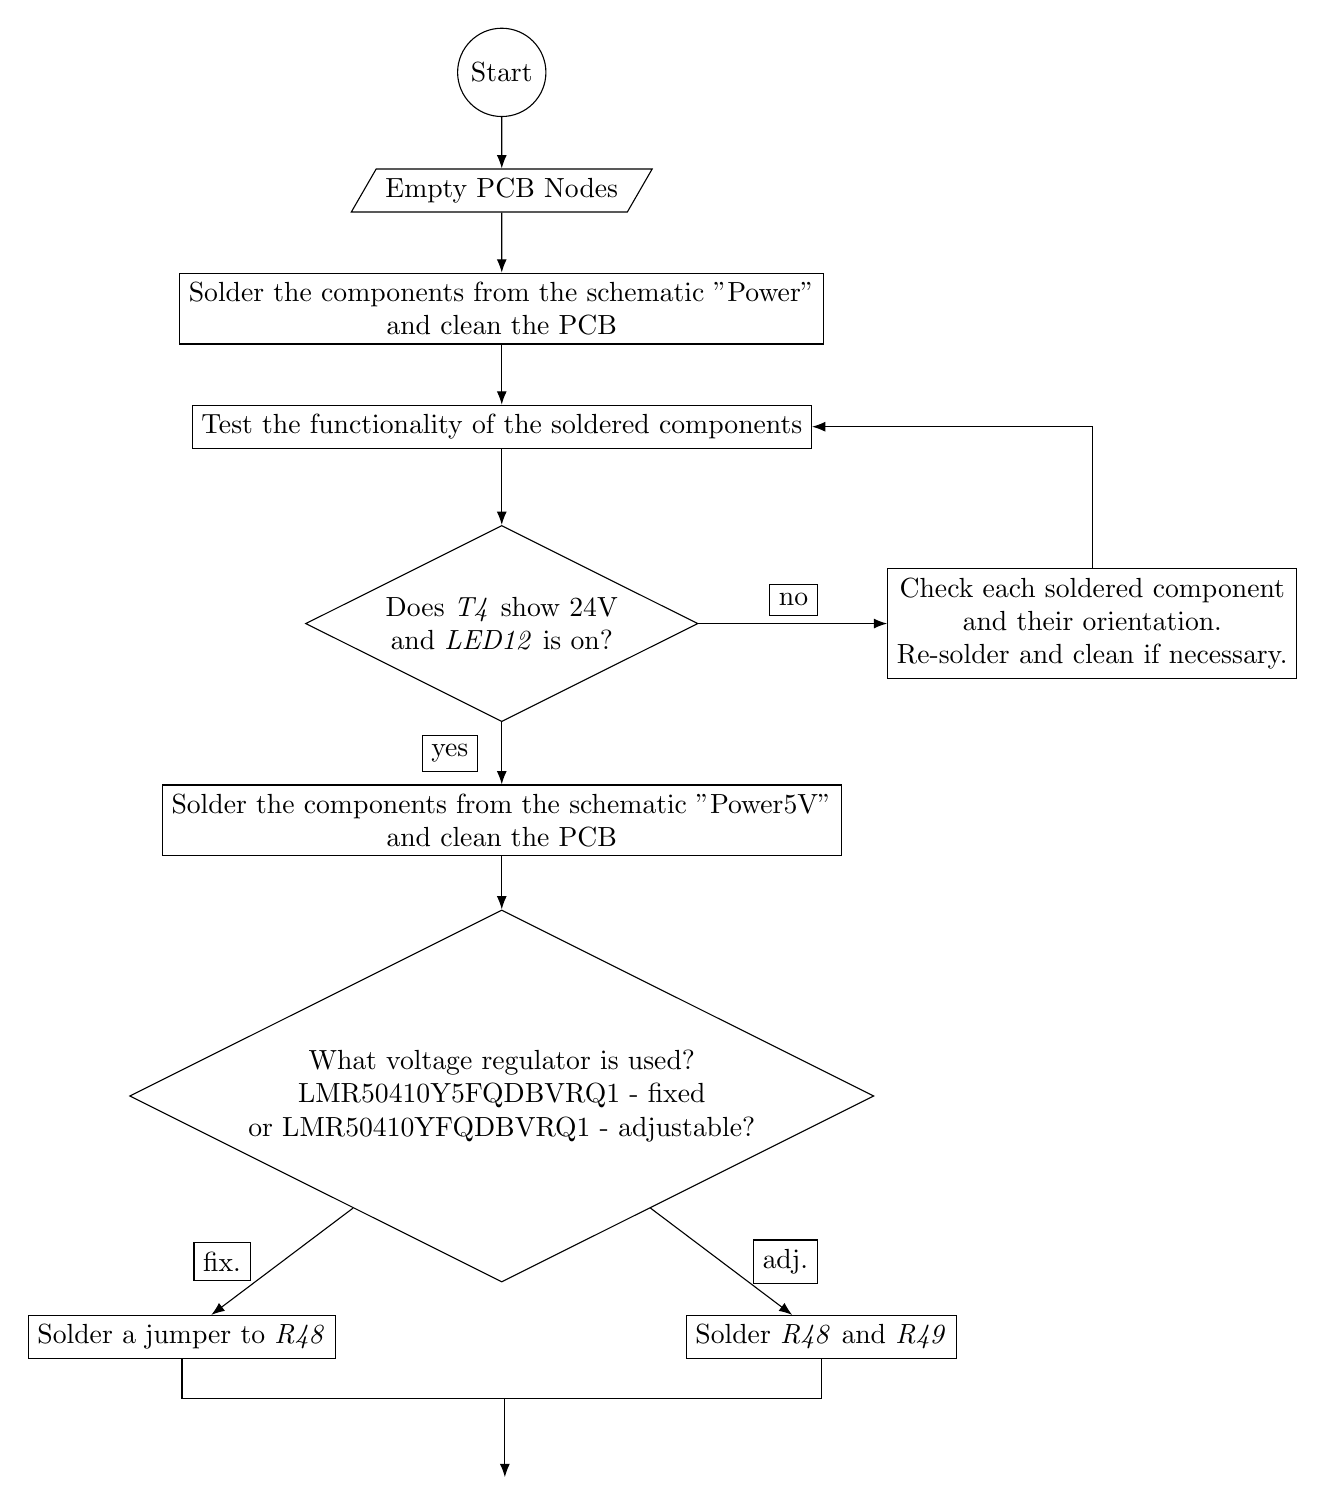
\begin{tikzpicture}[
    ->, >=Latex, node distance=1.5cm, every node/.style={draw, align=center}
]
% Define shapes
\node (start) [circle] {Start};
\node (input) [trapezium, below of=start, trapezium left angle=60, trapezium right angle=120] {Empty PCB Nodes};
\node (solder_power) [rectangle, below of=input] {Solder the components from the schematic "Power"\\ and clean the PCB};
\node (test_power) [rectangle, below of=solder_power] {Test the functionality of the soldered components};

\node (condition_power) [diamond, aspect=2, below of=test_power, yshift=-1cm] {Does \textit{T4} show 24V\\ and \textit{LED12} is on?};
\node (yes_power_5v) [rectangle, below of=condition_power, yshift=-1cm] {Solder the components from the schematic "Power5V"\\and clean the PCB};
\node (no_power) [rectangle, right of=condition_power, xshift=6cm] {Check each soldered component\\ and their orientation. \\ Re-solder and clean if necessary.};

\node (condition_power_5v_reg) [diamond, aspect=2, below of=yes_power_5v, yshift=-2cm] {What voltage regulator is used?\\
LMR50410Y5FQDBVRQ1 - fixed\\ or LMR50410YFQDBVRQ1 - adjustable?};
\node (fix_power_5v_reg) [rectangle, below left of=condition_power_5v_reg, xshift=-3cm, yshift=-2cm] {Solder a jumper to \textit{R48}};
\node (adj_power_5v_reg) [rectangle, below right of=condition_power_5v_reg, xshift=3cm, yshift=-2cm] {Solder \textit{R48} and \textit{R49}};
%\coordinate (toProcess2_1) at (fix_power_5v_reg.south);
%\coordinate (toProcess2_2) at (adj_power_5v_reg.south);
% Draw arrows
\draw[->] (start) -- (input);
\draw[->] (input) -- (solder_power);
\draw[->] (solder_power) -- (test_power);
\draw[->] (test_power) -- (condition_power);
\draw[->] (condition_power) -- node[left, xshift=-0.3cm] {yes} (yes_power_5v);
\draw[->] (condition_power) -- node[right, xshift=-0.3cm, yshift=0.3cm] {no} (no_power);
\draw[->] (yes_power_5v) -- (condition_power_5v_reg);
\draw[->] (no_power) |- (test_power);
\draw[->] (condition_power_5v_reg) -- node[left, xshift=-0.4cm] {fix.}(fix_power_5v_reg);
\draw[->] (condition_power_5v_reg) -- node[right, xshift=0.4cm] {adj.} (adj_power_5v_reg);
\draw[-] (adj_power_5v_reg.south) -- ++(0,-0.5) -- ++(-4.1,0);
\draw[->] (fix_power_5v_reg.south) -- ++(0,-0.5) -- ++(4.1,0) -- ++(0,-1);
\end{tikzpicture}
\end{center}
\newpage
\begin{center}
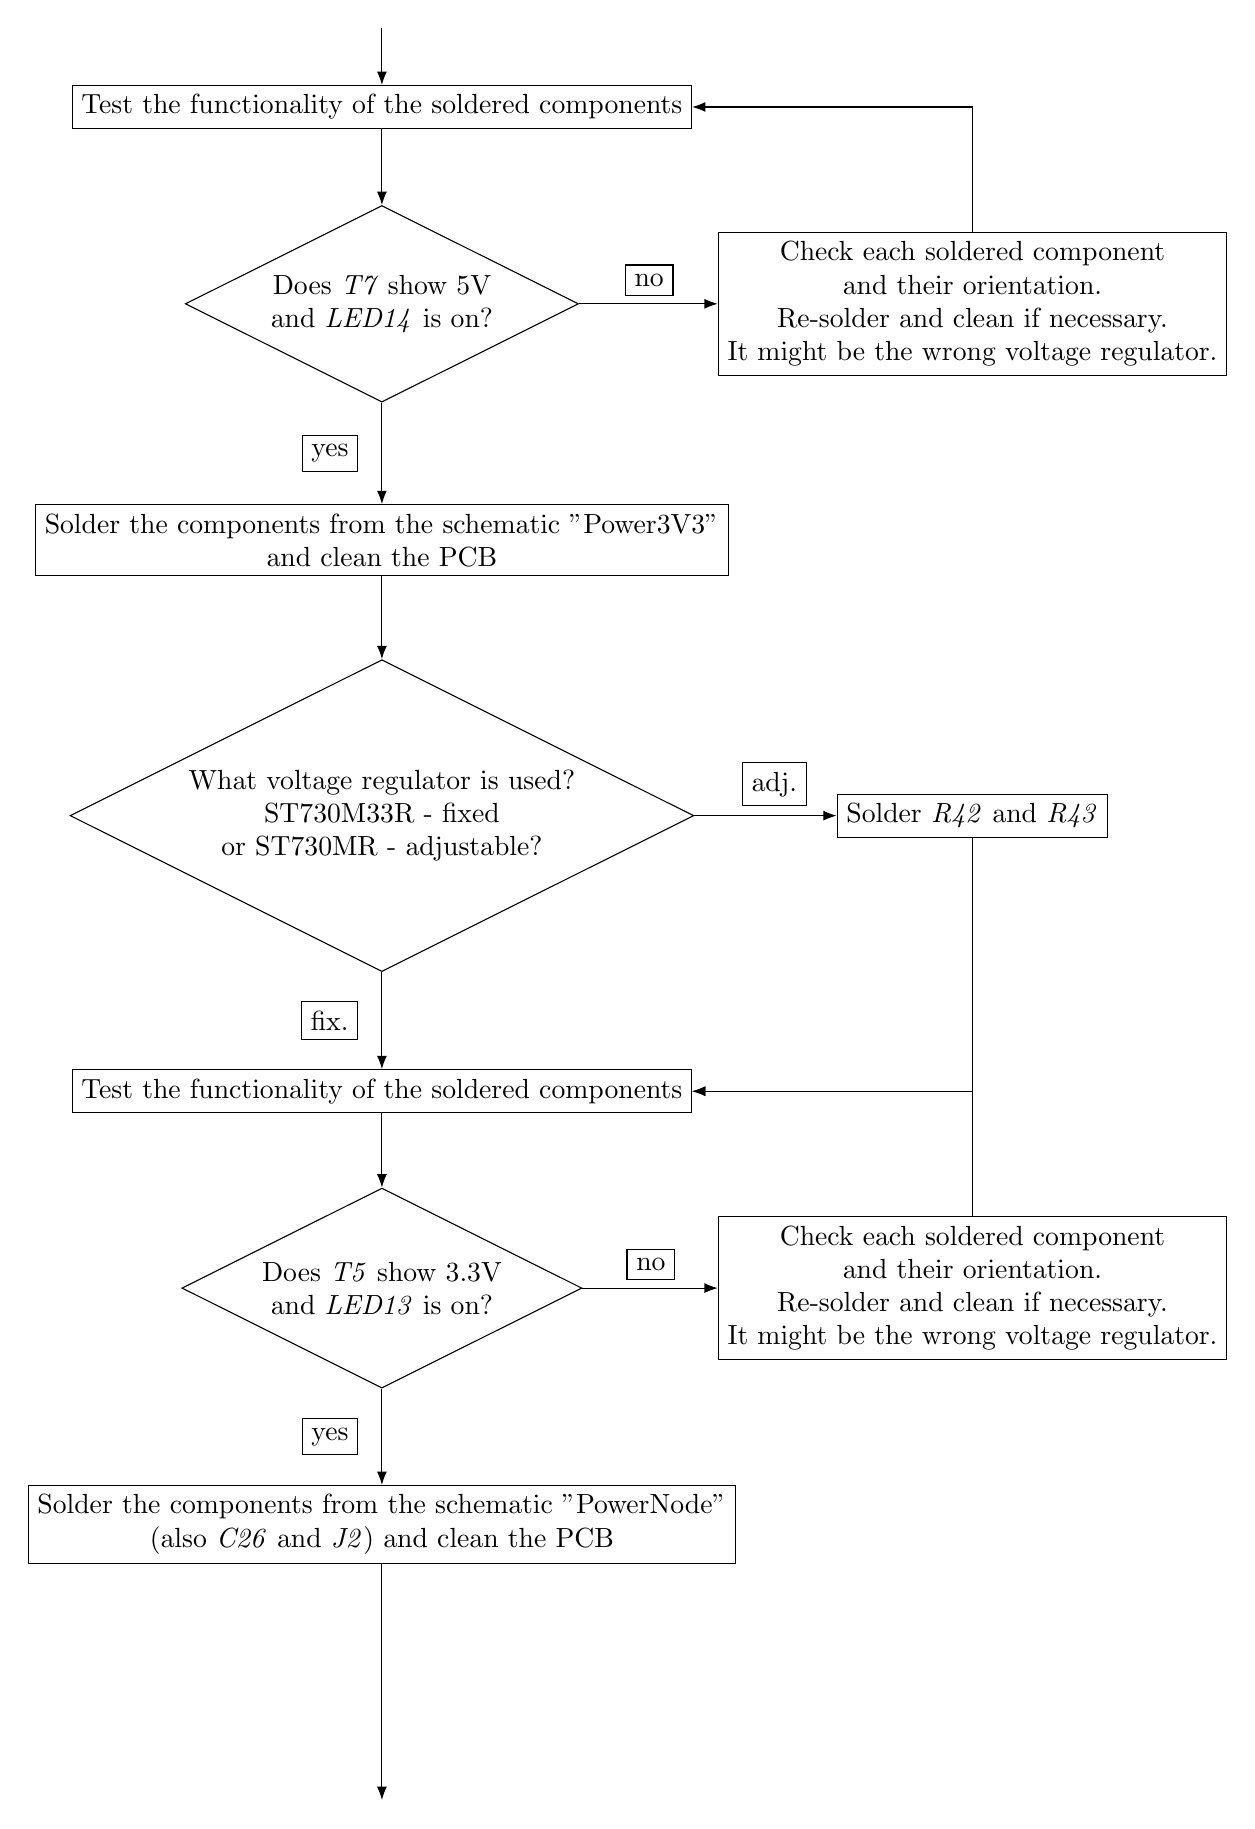
\begin{tikzpicture}[
    ->, >=Latex, node distance=1.5cm, every node/.style={draw, align=center}
]
\node (test_power_5v) [rectangle] {Test the functionality of the soldered components};
\node (condition_power_5v) [diamond, aspect=2, below of=test_power_5v, yshift=-1cm] {Does \textit{T7} show 5V\\ and \textit{LED14} is on?};
\node (yes_power_3v3) [rectangle, below of=condition_power_5v, yshift=-1.5cm] {Solder the components from the schematic "Power3V3"\\and clean the PCB};
\node (no_power_5v) [rectangle, right of=condition_power_5v, xshift=6cm] {Check each soldered component\\ and their orientation. \\ Re-solder and clean if necessary.\\ It might be the wrong voltage regulator.};

\node (condition_power_3v3_reg) [diamond, aspect=2, below of=yes_power_3v3, yshift=-2cm] {What voltage regulator is used?\\
ST730M33R - fixed\\ or ST730MR - adjustable?};
\node (test_power_3v3) [rectangle, below of=condition_power_3v3_reg, yshift=-2cm] {Test the functionality of the soldered components};
\node (adj_power_3v3_reg) [rectangle, right of=condition_power_3v3_reg, xshift=6cm] {Solder \textit{R42} and \textit{R43}};

\node (condition_power_3v3) [diamond, aspect=2, below of=test_power_3v3, yshift=-1cm] {Does \textit{T5} show 3.3V\\ and \textit{LED13} is on?};
\node (yes_power_node) [rectangle, below of=condition_power_3v3, yshift=-1.5cm] {Solder the components from the schematic "PowerNode"\\ (also \textit{C26} and \textit{J2}) and clean the PCB};
\node (no_power_3v3) [rectangle, right of=condition_power_3v3, xshift=6cm] {Check each soldered component\\ and their orientation. \\ Re-solder and clean if necessary.\\ It might be the wrong voltage regulator.};

%\coordinate (fromfix) at (fix_power_5v_reg.north);
%\coordinate (fromadj) at (adj_power_5v_reg.north);
\draw[->] ++(0,1) -- (test_power_5v.north);
\draw[->] (test_power_5v) -- (condition_power_5v);
\draw[->] (condition_power_5v) -- node[left, xshift=-0.3cm] {yes} (yes_power_3v3);
\draw[->] (condition_power_5v) -- node[right, xshift=-0.3cm, yshift=0.3cm] {no} (no_power_5v);
\draw[->] (no_power_5v) |- (test_power_5v);
\draw[->] (yes_power_3v3) -- (condition_power_3v3_reg);
\draw[->] (condition_power_3v3_reg) -- node[left, xshift=-0.3cm] {fix.}(test_power_3v3);
\draw[->] (condition_power_3v3_reg) -- node[right, xshift=-0.3cm, yshift=0.4cm] {adj.}(adj_power_3v3_reg);
\draw[->] (adj_power_3v3_reg) |- (test_power_3v3);
\draw[->] (test_power_3v3) -- (condition_power_3v3);
\draw[->] (condition_power_3v3) -- node[left, xshift=-0.3cm] {yes} (yes_power_node);
\draw[->] (condition_power_3v3) -- node[right, xshift=-0.3cm, yshift=0.3cm] {no} (no_power_3v3);
\draw[->] (no_power_3v3) |- (test_power_3v3);
\draw[->] (yes_power_node.south) -- ++(0,-3);
\end{tikzpicture}
\end{center}

\newpage
\begin{center}
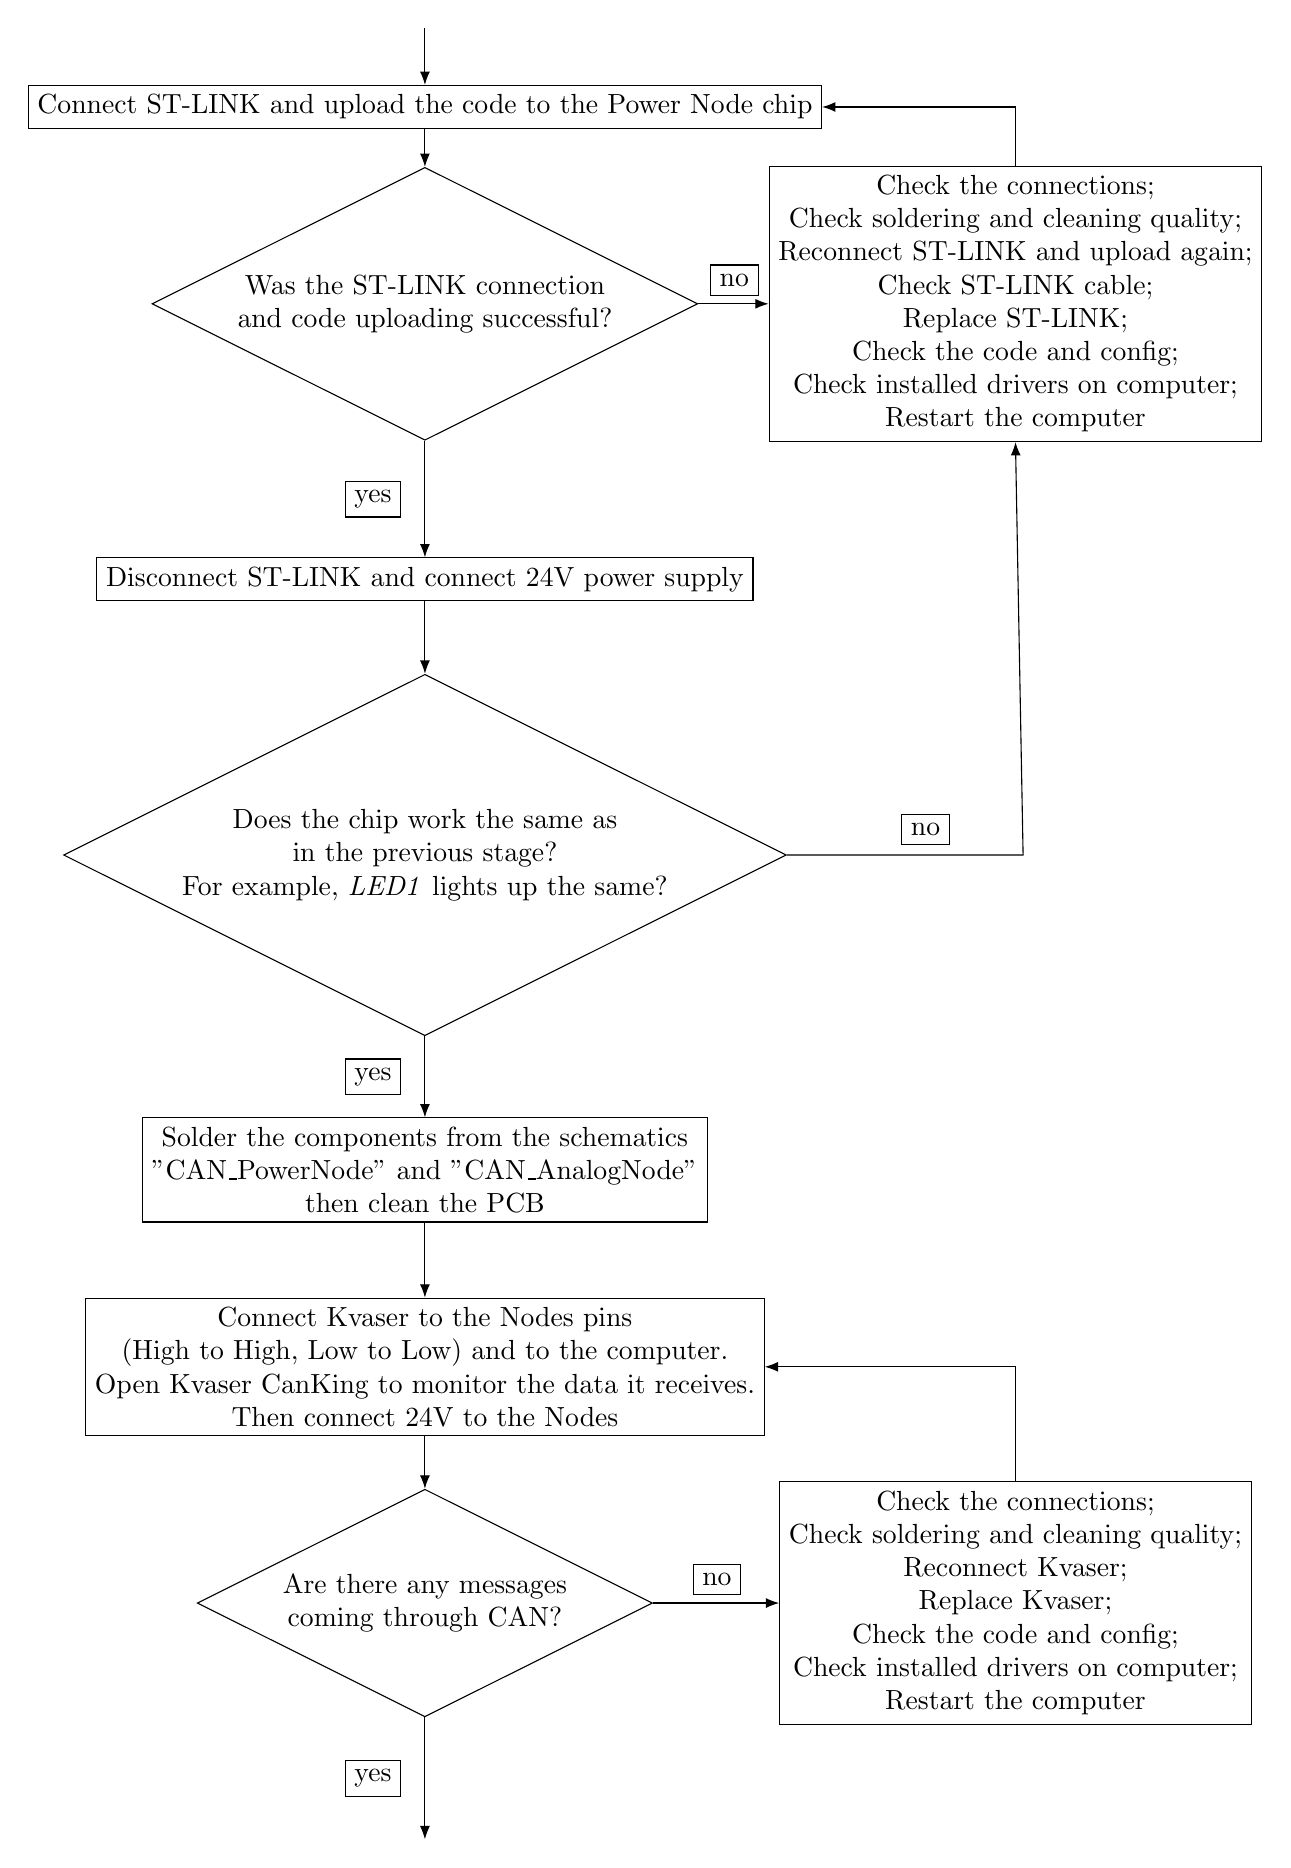
\begin{tikzpicture}[
    ->, >=Latex, node distance=1.5cm, every node/.style={draw, align=center}
]
\node (upload_power_node) [rectangle] {Connect ST-LINK and upload the code to the Power Node chip};
\node (condition_power_node_code) [diamond, aspect=2, below of=upload_power_node, yshift=-1cm] {Was the ST-LINK connection\\ and code uploading successful?};
\node (yes_power_node_code) [rectangle, below of=condition_power_node_code, yshift=-2cm] {Disconnect ST-LINK and connect 24V power supply};
\node (no_power_node_code) [rectangle, right of=condition_power_node_code, xshift=6cm] {Check the connections; \\Check soldering and cleaning quality; \\ Reconnect ST-LINK and upload again; \\Check ST-LINK cable;\\ Replace ST-LINK; \\Check the code and config; \\Check installed drivers on computer; \\Restart the computer};

\node (condition_power_node_power) [diamond, aspect=2, below of=yes_power_node_code, yshift=-2cm] {Does the chip work the same as \\in the previous stage?\\ For example, \textit{LED1} lights up the same?};
\node (yes_power_node_can) [rectangle, below of=condition_power_node_power, yshift=-2.5cm] {Solder the components from the schematics\\ "CAN\_PowerNode" and "CAN\_AnalogNode" \\then clean the PCB};
\node (power_node_can) [rectangle, below of=yes_power_node_can, yshift=-1cm] {Connect Kvaser to the Nodes pins \\(High to High, Low to Low) and to the computer. \\Open Kvaser CanKing to monitor the data it receives. \\Then connect 24V to the Nodes};

\node (condition_power_node_can) [diamond, aspect=2, below of=power_node_can, yshift=-1.5cm] {Are there any messages\\ coming through CAN?};
\node (no_power_node_can) [rectangle, right of=condition_power_node_can, xshift=6cm] {Check the connections; \\Check soldering and cleaning quality; \\ Reconnect Kvaser; \\ Replace Kvaser; \\Check the code and config; \\Check installed drivers on computer; \\Restart the computer};
\draw[->] ++(0,1) -- (upload_power_node.north);
\draw[->] (upload_power_node) -- (condition_power_node_code);
\draw[->] (condition_power_node_code) -- node[left, xshift=-0.3cm] {yes} (yes_power_node_code);
\draw[->] (condition_power_node_code) -- node[right, xshift=-0.3cm, yshift=0.3cm] {no} (no_power_node_code);
\draw[->] (no_power_node_code) |- (upload_power_node);

\draw[->] (yes_power_node_code) -- (condition_power_node_power);
\draw[->] (condition_power_node_power) -- node[left, xshift=-0.3cm] {yes} (yes_power_node_can);
\draw[->] (condition_power_node_power.east) |- ++(3,0) -- node[right, xshift=-1.5cm, yshift=-2.3cm] {no} (no_power_node_code.south);

\draw[->] (yes_power_node_can) -- (power_node_can);
\draw[->] (power_node_can) -- (condition_power_node_can);
\draw[->] (condition_power_node_can) -- node[left, xshift=-0.3cm] {yes} ++(0,-3);
\draw[->] (condition_power_node_can) -- node[right, xshift=-0.3cm, yshift=0.3cm] {no} (no_power_node_can);
\draw[->] (no_power_node_can) |- (power_node_can);
\end{tikzpicture}
\end{center}
\newpage
\begin{center}
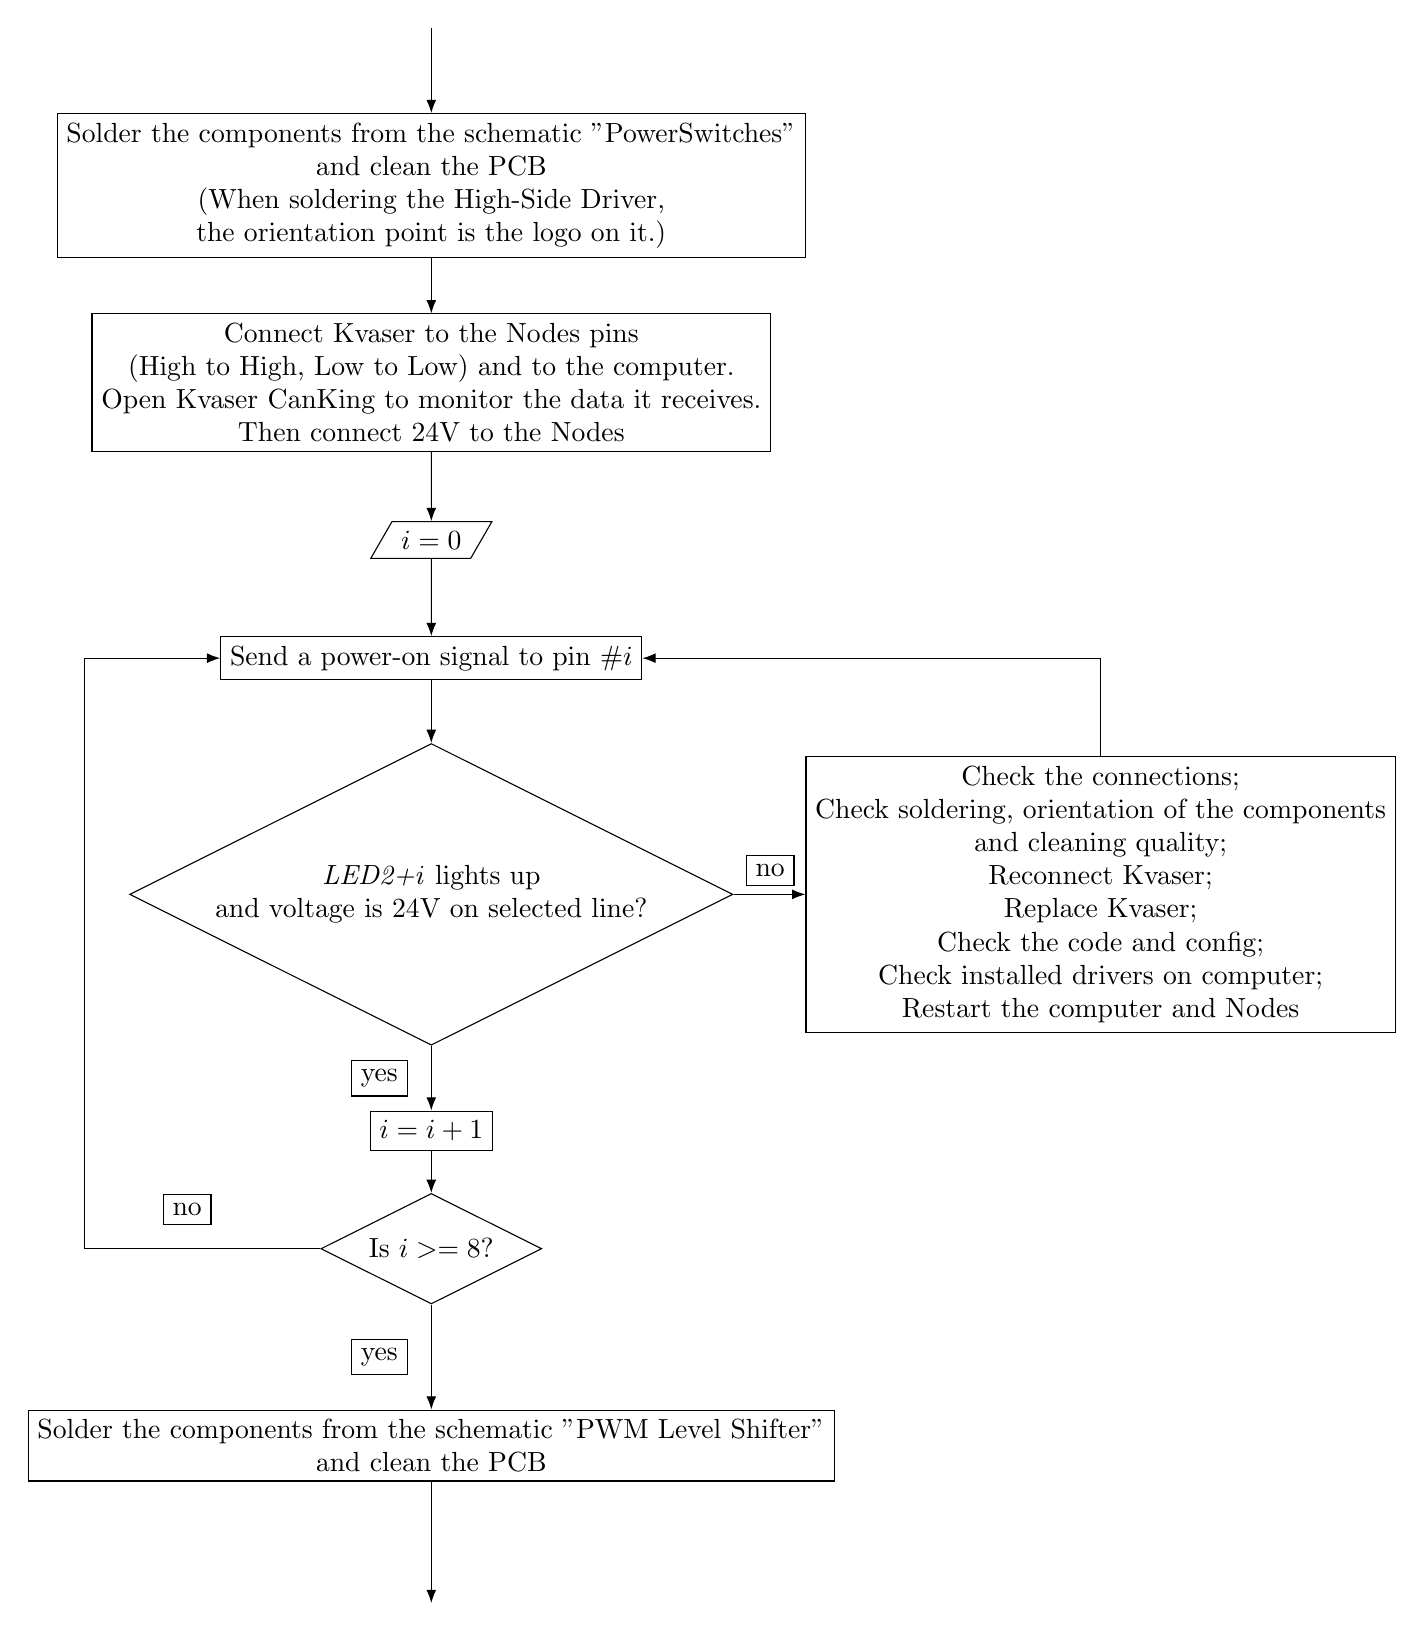
\begin{tikzpicture}[
    ->, >=Latex, node distance=1.5cm, every node/.style={draw, align=center}
]
\node (yes_power_node_switch) [rectangle] {Solder the components from the schematic "PowerSwitches"\\ and clean the PCB\\ (When soldering the High-Side Driver,\\ the orientation point is the logo on it.)};
\node (test_power_node_switch) [rectangle, below of=yes_power_node_switch, yshift=-1cm] {Connect Kvaser to the Nodes pins \\(High to High, Low to Low) and to the computer. \\Open Kvaser CanKing to monitor the data it receives. \\Then connect 24V to the Nodes};
\node (try_value) [trapezium, below of=test_power_node_switch, trapezium left angle=60, trapezium right angle=120, yshift=-0.5cm] {$i = 0$};
\node (test_power_node_switch_change) [rectangle, below of=try_value] {Send a power-on signal to pin $\#i$};
\node (condition_power_node_switch) [diamond, aspect=2, below of=test_power_node_switch_change, yshift=-1.5cm] {\textit{LED2+i} lights up\\ and voltage is 24V on selected line?};
\node (no_power_node_switch) [rectangle, right of=condition_power_node_switch, xshift=7cm] {Check the connections; \\Check soldering, orientation of the components\\ and cleaning quality; \\ Reconnect Kvaser; \\ Replace Kvaser; \\Check the code and config; \\Check installed drivers on computer; \\Restart the computer and Nodes};
\node (yes_power_node_switch_change) [rectangle, below of=condition_power_node_switch, yshift=-1.5cm] {$i=i+1$};
\node (condition_power_node_switch_i) [diamond, aspect=2, below of=yes_power_node_switch_change] {Is $i>=8$?};
\node (yes_power_node_pwm) [rectangle, below of=condition_power_node_switch_i, yshift=-1cm] {Solder the components from the schematic "PWM Level Shifter"\\ and clean the PCB};
\draw[->] ++(0,2) -- (yes_power_node_switch.north);
\draw[->] (yes_power_node_switch) -- (test_power_node_switch);
\draw[->] (test_power_node_switch) -- (try_value);
\draw[->] (try_value) -- (test_power_node_switch_change);
\draw[->] (test_power_node_switch_change) -- (condition_power_node_switch);
\draw[->] (condition_power_node_switch) -- node[right, xshift=-0.3cm, yshift=0.3cm] {no} (no_power_node_switch);
\draw[->] (no_power_node_switch) |- (test_power_node_switch_change);
\draw[->] (condition_power_node_switch) -- node[left, xshift=-0.3cm] {yes} (yes_power_node_switch_change);
\draw[->] (yes_power_node_switch_change) -- (condition_power_node_switch_i);
\draw[->] (condition_power_node_switch_i.west) --++(-3,0) |- node[right, xshift=1cm, yshift=-7cm] {no} (test_power_node_switch_change);
\draw[->] (condition_power_node_switch_i) -- node[left, xshift=-0.3cm] {yes} (yes_power_node_pwm);
\draw[->] (yes_power_node_pwm) -- ++(0,-2);
\end{tikzpicture}
\end{center}
\newpage
\begin{center}
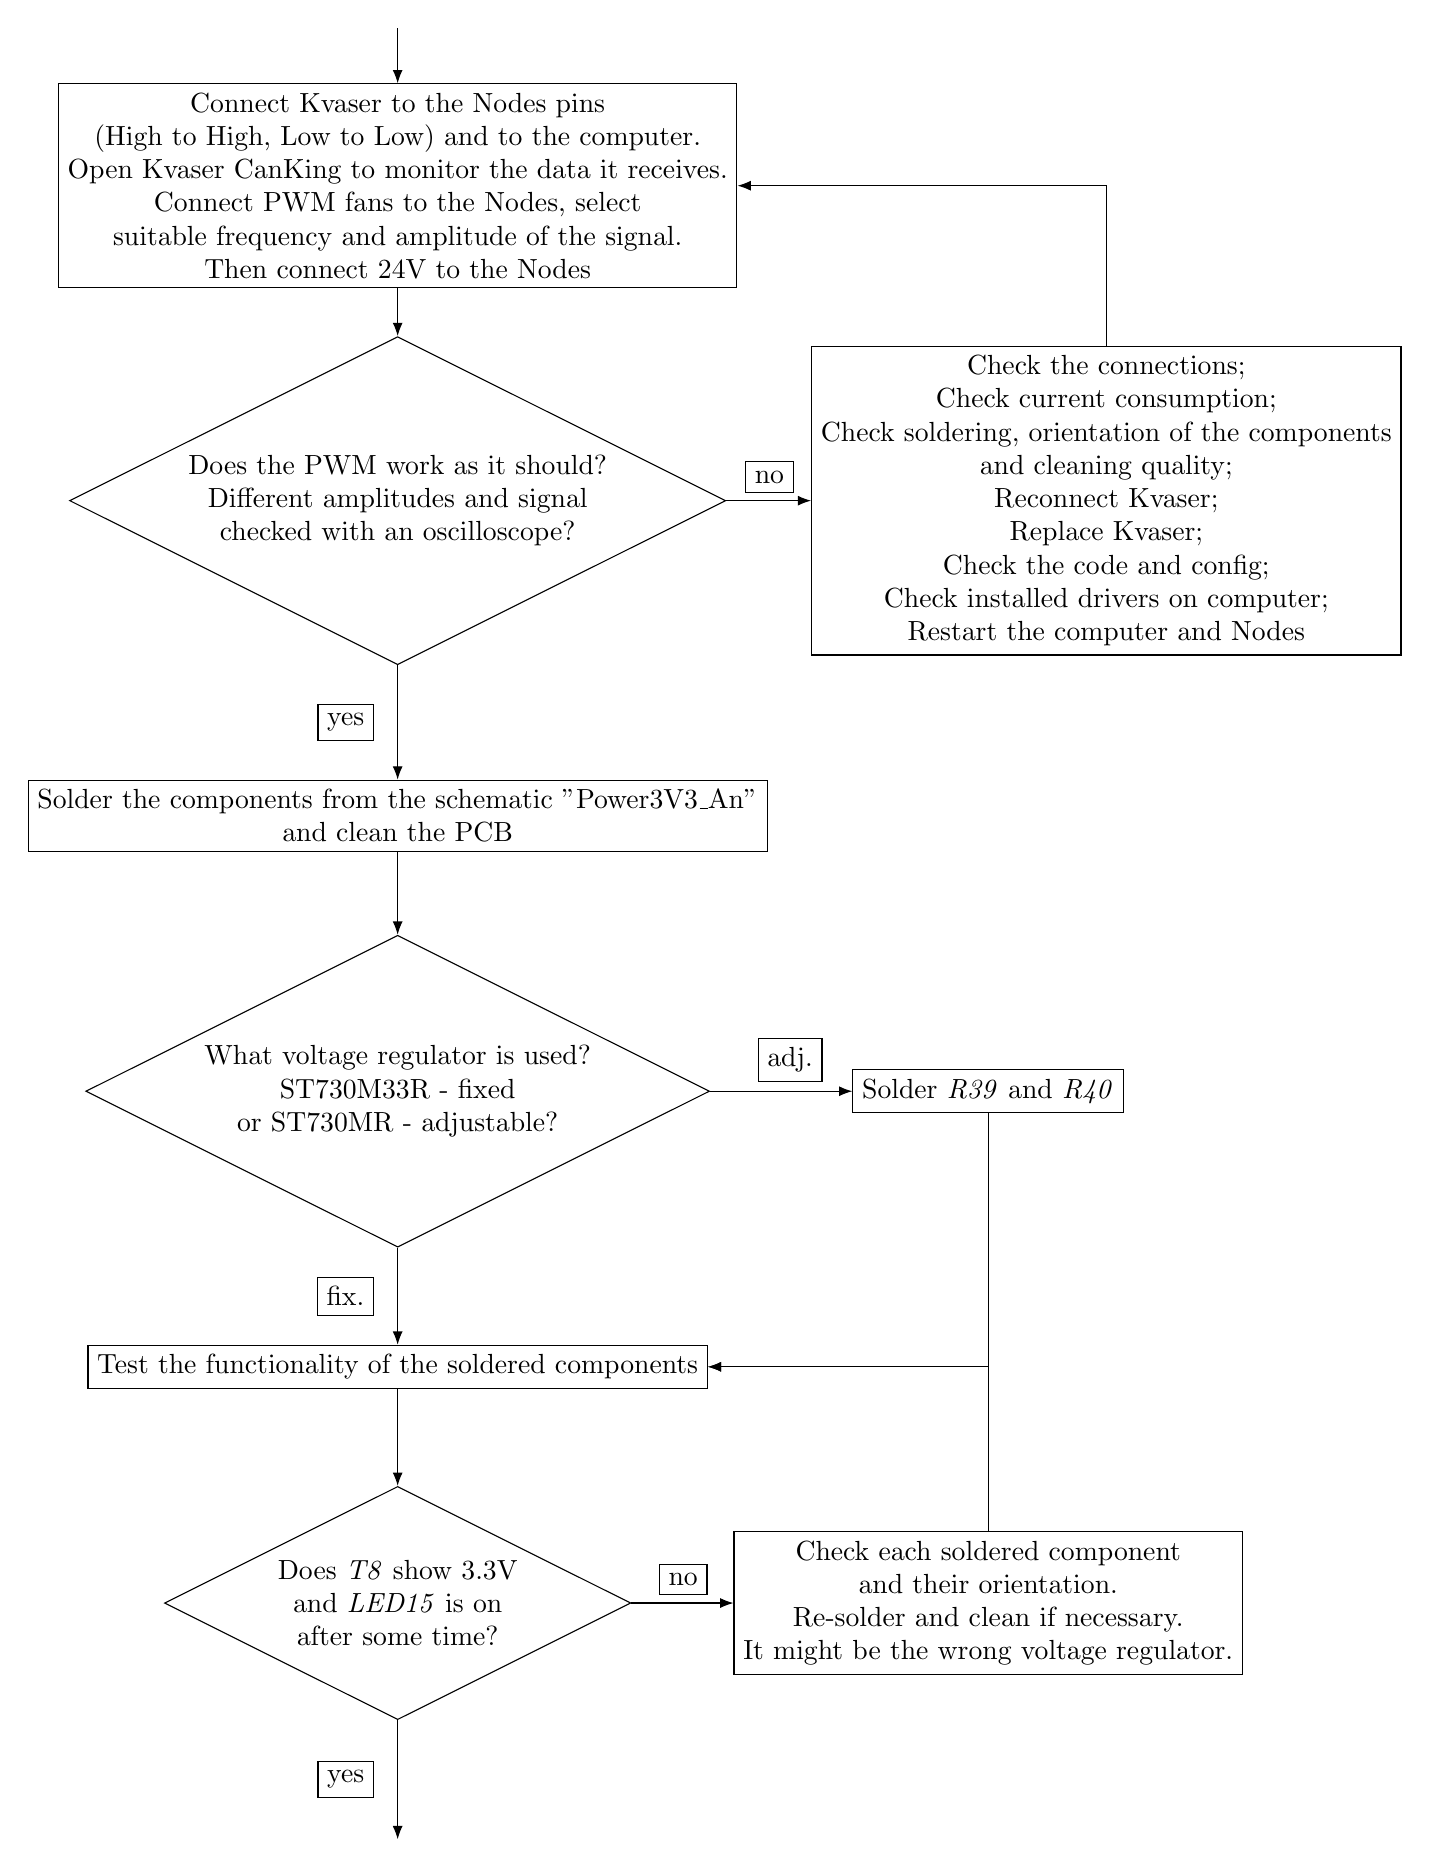
\begin{tikzpicture}[
    ->, >=Latex, node distance=1.5cm, every node/.style={draw, align=center}
]
\node (test_power_node_pwm) [rectangle] {Connect Kvaser to the Nodes pins \\(High to High, Low to Low) and to the computer. \\Open Kvaser CanKing to monitor the data it receives. \\Connect PWM fans to the Nodes, select \\suitable frequency and amplitude of the signal. \\Then connect 24V to the Nodes};
\node (condition_power_node_pwm) [diamond, below of = test_power_node_pwm, aspect=2, yshift=-2.5cm] {Does the PWM work as it should?\\ Different amplitudes and signal \\checked with an oscilloscope?};
\node (yes_power_3v3_an) [rectangle, below of=condition_power_node_pwm, yshift=-2.5cm] {Solder the components from the schematic "Power3V3\_An"\\ and clean the PCB};
\node (no_power_node_pwm) [rectangle, right of=condition_power_node_pwm, xshift=7.5cm] {Check the connections; \\ Check current consumption; \\Check soldering, orientation of the components\\ and cleaning quality; \\ Reconnect Kvaser; \\ Replace Kvaser; \\Check the code and config; \\Check installed drivers on computer; \\Restart the computer and Nodes};
\node (condition_power_3v3_an_reg) [diamond, aspect=2, below of=yes_power_3v3_an, yshift=-2cm] {What voltage regulator is used?\\
ST730M33R - fixed\\ or ST730MR - adjustable?};
\node (test_power_3v3_an) [rectangle, below of=condition_power_3v3_an_reg, yshift=-2cm] {Test the functionality of the soldered components};
\node (adj_power_3v3_an_reg) [rectangle, right of=condition_power_3v3_an_reg, xshift=6cm] {Solder \textit{R39} and \textit{R40}};
\node (condition_power_3v3_an) [diamond, aspect=2, below of=test_power_3v3_an, yshift=-1.5cm] {Does \textit{T8} show 3.3V\\ and \textit{LED15} is on \\after some time?};
\node (no_power_3v3_an) [rectangle, right of=condition_power_3v3_an, xshift=6cm] {Check each soldered component\\ and their orientation. \\ Re-solder and clean if necessary.\\ It might be the wrong voltage regulator.};
\draw[->] ++(0,2) -- (test_power_node_pwm.north);
\draw[->] (test_power_node_pwm) -- (condition_power_node_pwm);
\draw[->] (condition_power_node_pwm.east) -- node[right, xshift=-0.3cm, yshift=0.3cm] {no} (no_power_node_pwm);
\draw[->] (no_power_node_pwm) |- (test_power_node_pwm);
\draw[->] (condition_power_node_pwm) -- node[left, xshift=-0.3cm] {yes} (yes_power_3v3_an);
\draw[->] (yes_power_3v3_an) -- (condition_power_3v3_an_reg);
\draw[->] (condition_power_3v3_an_reg) -- node[left, xshift=-0.3cm] {fix.}(test_power_3v3_an);
\draw[->] (condition_power_3v3_an_reg) -- node[right, xshift=-0.3cm, yshift=0.4cm] {adj.}(adj_power_3v3_an_reg);
\draw[->] (adj_power_3v3_an_reg) |- (test_power_3v3_an);
\draw[->] (test_power_3v3_an) -- (condition_power_3v3_an);
\draw[->] (condition_power_3v3_an.east) -- node[right, xshift=-0.3cm, yshift=0.3cm] {no} (no_power_3v3_an);
\draw[->] (no_power_3v3_an) |- (test_power_3v3_an);
\draw[->] (condition_power_3v3_an) -- node[left, xshift=-0.3cm] {yes} ++(0,-3);
\end{tikzpicture}
\end{center}

\newpage
\begin{center}
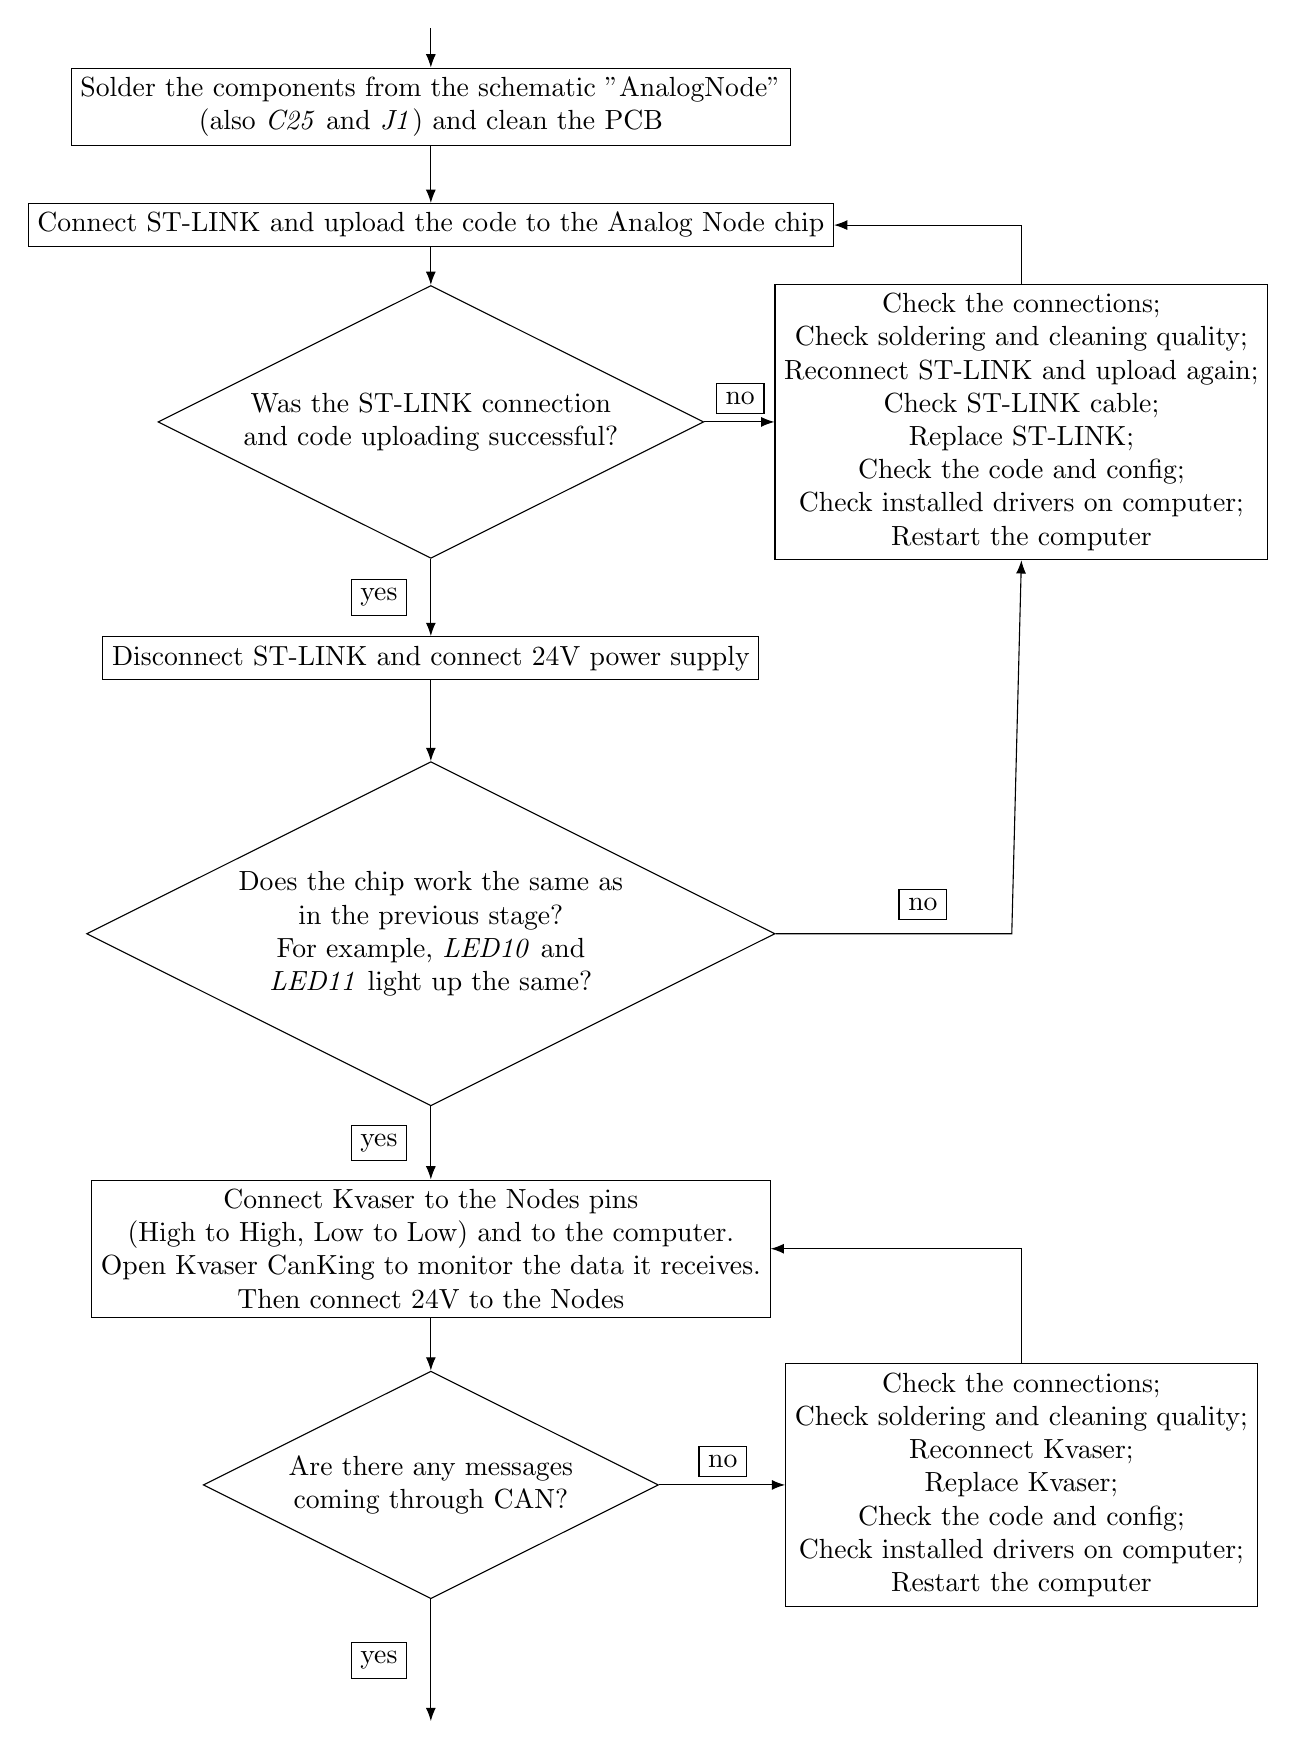
\begin{tikzpicture}[
    ->, >=Latex, node distance=1.5cm, every node/.style={draw, align=center}
]
\node (yes_analog_node) [rectangle] {Solder the components from the schematic "AnalogNode"\\ (also \textit{C25} and \textit{J1}) and clean the PCB};
\node (upload_analog_node) [rectangle, below of=yes_analog_node] {Connect ST-LINK and upload the code to the Analog Node chip};
\node (condition_analog_node_code) [diamond, aspect=2, below of=upload_analog_node, yshift=-1cm] {Was the ST-LINK connection\\ and code uploading successful?};
\node (yes_analog_node_code) [rectangle, below of=condition_analog_node_code, yshift=-1.5cm] {Disconnect ST-LINK and connect 24V power supply};
\node (no_analog_node_code) [rectangle, right of=condition_analog_node_code, xshift=6cm] {Check the connections; \\Check soldering and cleaning quality; \\ Reconnect ST-LINK and upload again; \\Check ST-LINK cable;\\ Replace ST-LINK; \\Check the code and config; \\Check installed drivers on computer; \\Restart the computer};

\node (condition_analog_node_power) [diamond, aspect=2, below of=yes_analog_node_code, yshift=-2cm] {Does the chip work the same as \\in the previous stage?\\ For example, \textit{LED10} and \\\textit{LED11} light up the same?};
\node (analog_node_can) [rectangle, below of=condition_analog_node_power, yshift=-2.5cm] {Connect Kvaser to the Nodes pins \\(High to High, Low to Low) and to the computer. \\Open Kvaser CanKing to monitor the data it receives. \\Then connect 24V to the Nodes};

\node (condition_analog_node_can) [diamond, aspect=2, below of=analog_node_can, yshift=-1.5cm] {Are there any messages\\ coming through CAN?};
\node (no_analog_node_can) [rectangle, right of=condition_analog_node_can, xshift=6cm] {Check the connections; \\Check soldering and cleaning quality; \\ Reconnect Kvaser; \\ Replace Kvaser; \\Check the code and config; \\Check installed drivers on computer; \\Restart the computer};

\draw[->] ++(0,1) -- (yes_analog_node.north);
\draw[->] (yes_analog_node) -- (upload_analog_node);
\draw[->] (upload_analog_node) -- (condition_analog_node_code);
\draw[->] (condition_analog_node_code) -- node[left, xshift=-0.3cm] {yes} (yes_analog_node_code);
\draw[->] (condition_analog_node_code) -- node[right, xshift=-0.3cm, yshift=0.3cm] {no} (no_analog_node_code);
\draw[->] (no_analog_node_code) |- (upload_analog_node);

\draw[->] (yes_analog_node_code) -- (condition_analog_node_power);
\draw[->] (condition_analog_node_power) -- node[left, xshift=-0.3cm] {yes} (analog_node_can);
\draw[->] (condition_analog_node_power.east) |- ++(3,0) -- node[right, xshift=-1.5cm, yshift=-2cm] {no} (no_analog_node_code.south);

\draw[->] (analog_node_can) -- (condition_analog_node_can);
\draw[->] (condition_analog_node_can) -- node[left, xshift=-0.3cm] {yes} ++(0,-3);
\draw[->] (condition_analog_node_can) -- node[right, xshift=-0.3cm, yshift=0.3cm] {no} (no_analog_node_can);
\draw[->] (no_analog_node_can) |- (analog_node_can);
\end{tikzpicture}
\end{center}

\newpage
\begin{center}
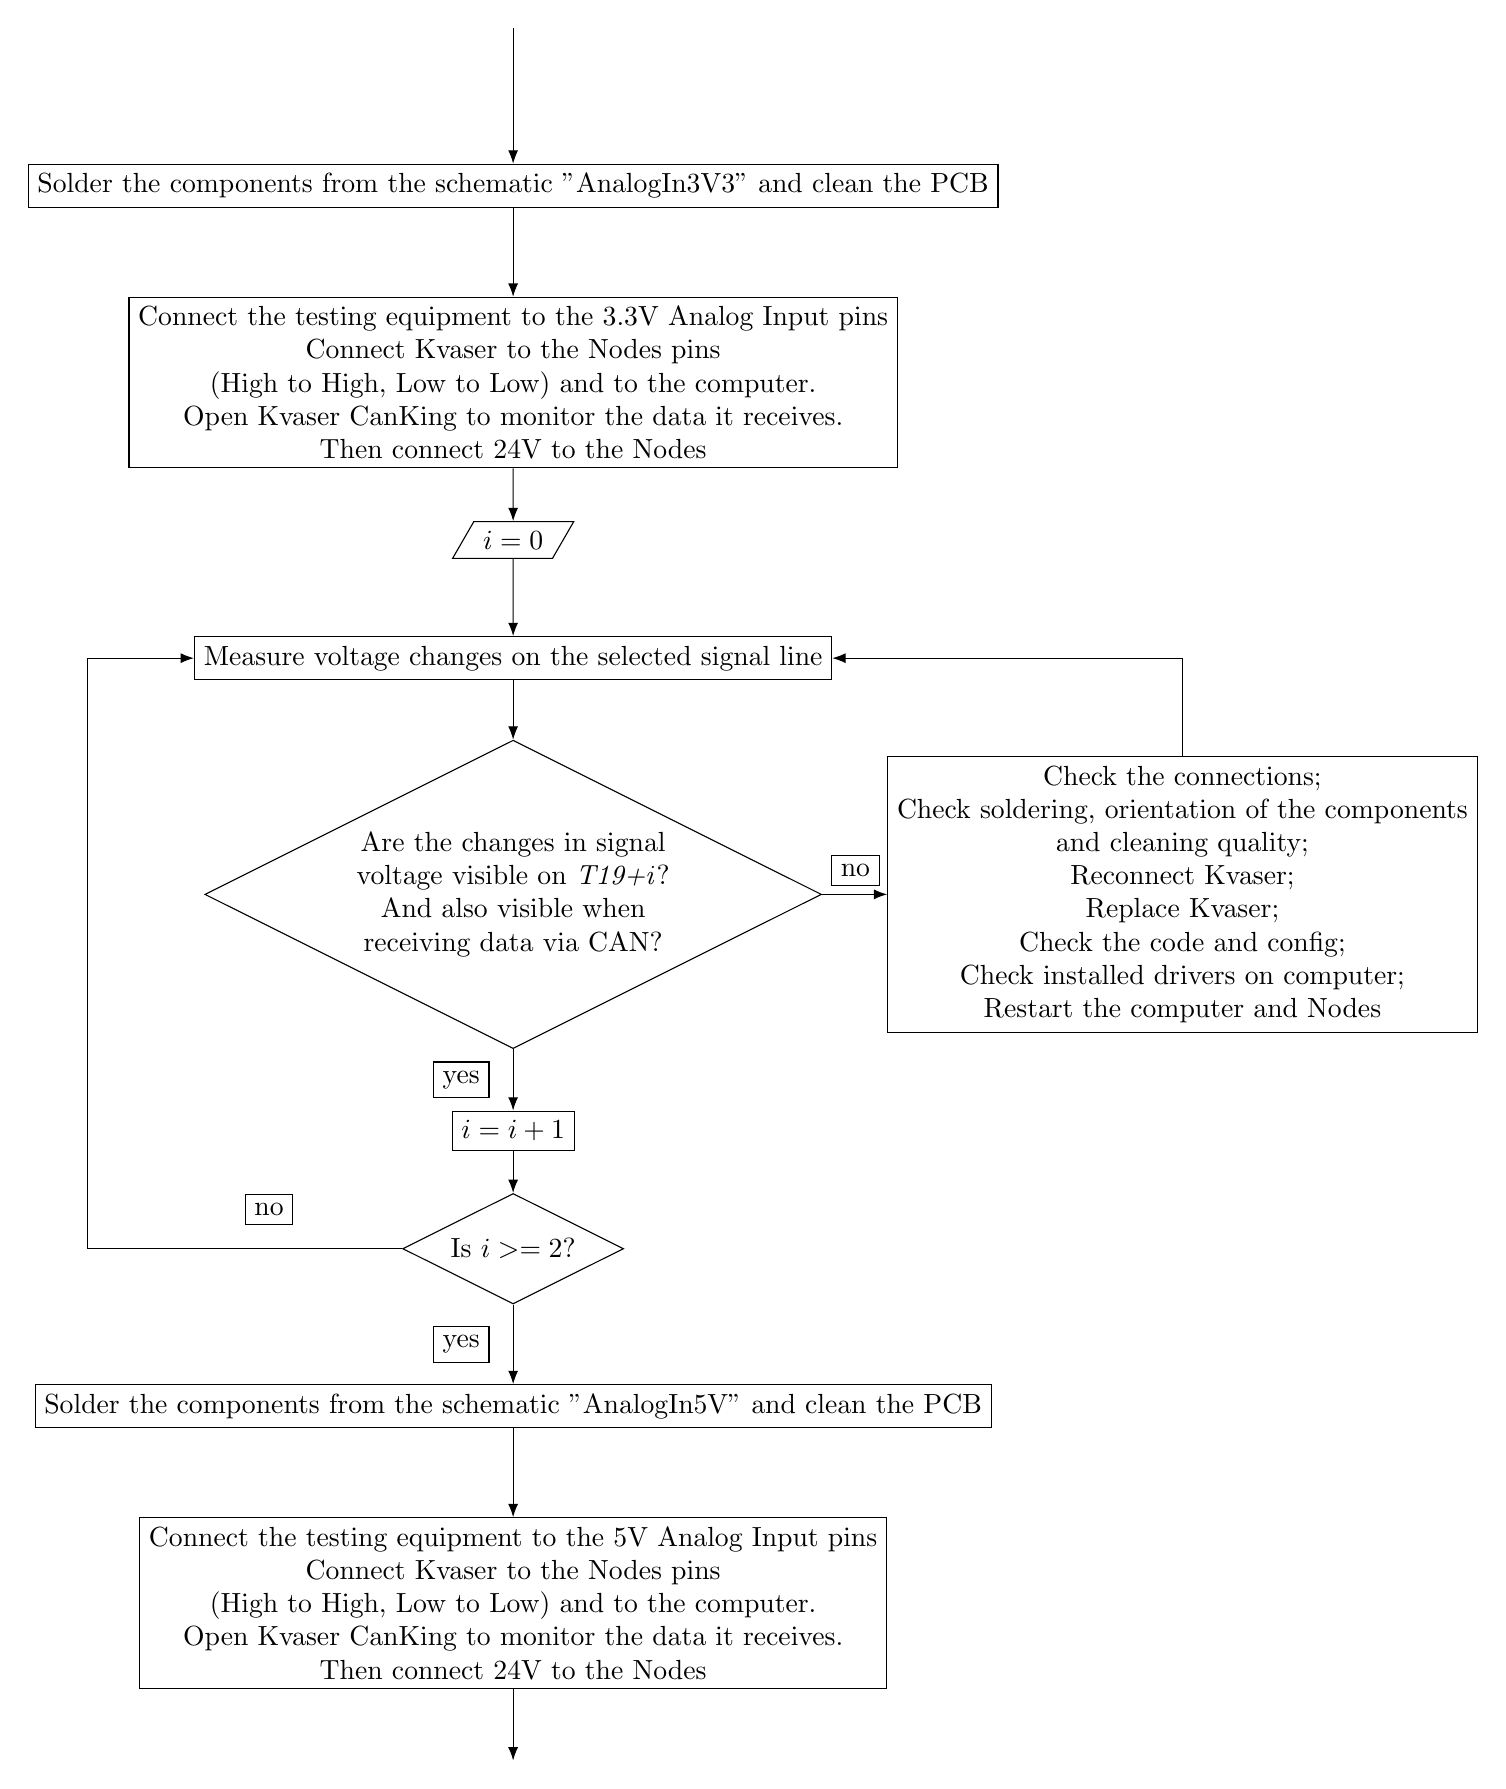
\begin{tikzpicture}[
    ->, >=Latex, node distance=1.5cm, every node/.style={draw, align=center}
]
\node (filters_3v3) [rectangle] {Solder the components from the schematic "AnalogIn3V3" and clean the PCB};
\node (test_filters_3v3) [rectangle, below of=filters_3v3, yshift=-1cm] {Connect the testing equipment to the 3.3V Analog Input pins\\ Connect Kvaser to the Nodes pins \\(High to High, Low to Low) and to the computer. \\Open Kvaser CanKing to monitor the data it receives. \\Then connect 24V to the Nodes};
\node (try_value_filters_3v3) [trapezium, below of=test_filters_3v3, trapezium left angle=60, trapezium right angle=120, yshift=-0.5cm] {$i = 0$};
\node (measure_filters_3v3) [rectangle, below of=try_value_filters_3v3] {Measure voltage changes on the selected signal line};
\node (condition_filters_3v3) [diamond, aspect=2, below of=measure_filters_3v3, yshift=-1.5cm] {Are the changes in signal \\voltage visible on \textit{T19+i}?\\ And also visible when \\receiving data via CAN?};
\node (no_filters_3v3) [rectangle, right of=condition_filters_3v3, xshift=7cm] {Check the connections; \\Check soldering, orientation of the components\\ and cleaning quality; \\ Reconnect Kvaser; \\ Replace Kvaser; \\Check the code and config; \\Check installed drivers on computer; \\Restart the computer and Nodes};
\node (yes_filters_3v3_change) [rectangle, below of=condition_filters_3v3, yshift=-1.5cm] {$i=i+1$};
\node (condition_filters_3v3_i) [diamond, aspect=2, below of=yes_filters_3v3_change] {Is $i>=2$?};
\node (filters_5v) [rectangle, below of=condition_filters_3v3_i, yshift=-0.5cm] {Solder the components from the schematic "AnalogIn5V" and clean the PCB};
\node (test_filters_5v) [rectangle, below of=filters_5v, yshift=-1cm] {Connect the testing equipment to the 5V Analog Input pins\\ Connect Kvaser to the Nodes pins \\(High to High, Low to Low) and to the computer. \\Open Kvaser CanKing to monitor the data it receives. \\Then connect 24V to the Nodes};

\draw[->] ++(0,2) -- (filters_3v3.north);
\draw[->] (filters_3v3) -- (test_filters_3v3);
\draw[->] (test_filters_3v3) -- (try_value_filters_3v3);
\draw[->] (try_value_filters_3v3) -- (measure_filters_3v3);
\draw[->] (measure_filters_3v3) -- (condition_filters_3v3);
\draw[->] (condition_filters_3v3) -- node[right, xshift=-0.3cm, yshift=0.3cm] {no} (no_filters_3v3);
\draw[->] (no_filters_3v3) |- (measure_filters_3v3);
\draw[->] (condition_filters_3v3) -- node[left, xshift=-0.3cm] {yes} (yes_filters_3v3_change);
\draw[->] (yes_filters_3v3_change) -- (condition_filters_3v3_i);
\draw[->] (condition_filters_3v3_i.west) --++(-4,0) |- node[right, xshift=2cm, yshift=-7cm] {no} (measure_filters_3v3);
\draw[->] (condition_filters_3v3_i) -- node[left, xshift=-0.3cm] {yes} (filters_5v);
\draw[->] (filters_5v) -- (test_filters_5v);
\draw[->] (test_filters_5v) -- ++(0,-2);
\end{tikzpicture}
\end{center}

\newpage
\begin{center}
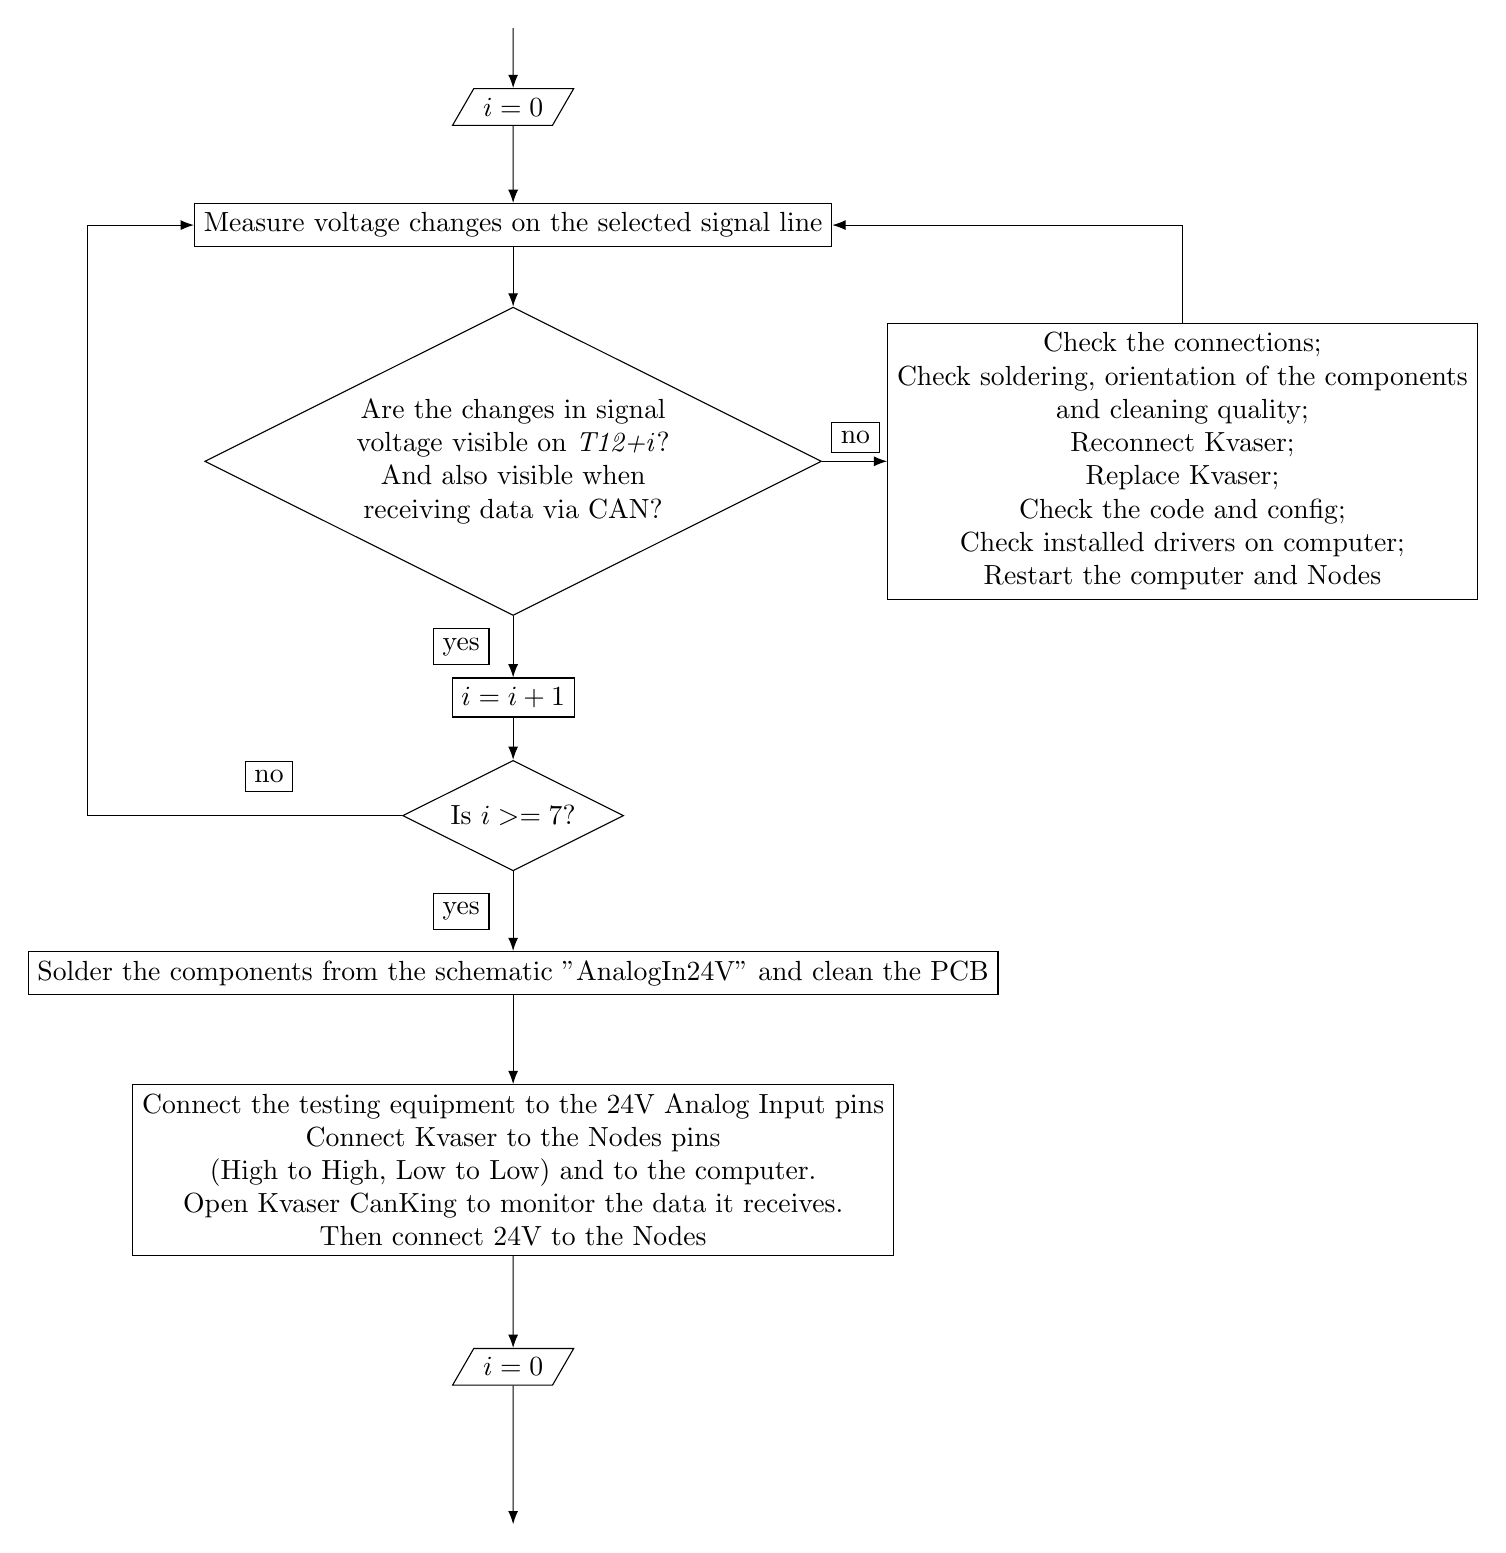
\begin{tikzpicture}[
    ->, >=Latex, node distance=1.5cm, every node/.style={draw, align=center}
]
\node (try_value_filters_5v) [trapezium, trapezium left angle=60, trapezium right angle=120] {$i = 0$};
\node (measure_filters_5v) [rectangle, below of=try_value_filters_5v] {Measure voltage changes on the selected signal line};
\node (condition_filters_5v) [diamond, aspect=2, below of=measure_filters_5v, yshift=-1.5cm] {Are the changes in signal \\voltage visible on \textit{T12+i}?\\ And also visible when \\receiving data via CAN?};
\node (no_filters_5v) [rectangle, right of=condition_filters_5v, xshift=7cm] {Check the connections; \\Check soldering, orientation of the components\\ and cleaning quality; \\ Reconnect Kvaser; \\ Replace Kvaser; \\Check the code and config; \\Check installed drivers on computer; \\Restart the computer and Nodes};
\node (yes_filters_5v_change) [rectangle, below of=condition_filters_5v, yshift=-1.5cm] {$i=i+1$};
\node (condition_filters_5v_i) [diamond, aspect=2, below of=yes_filters_5v_change] {Is $i>=7$?};
\node (filters_24v) [rectangle, below of=condition_filters_5v_i, yshift=-0.5cm] {Solder the components from the schematic "AnalogIn24V" and clean the PCB};
\node (test_filters_24v) [rectangle, below of=filters_24v, yshift=-1cm] {Connect the testing equipment to the 24V Analog Input pins\\ Connect Kvaser to the Nodes pins \\(High to High, Low to Low) and to the computer. \\Open Kvaser CanKing to monitor the data it receives. \\Then connect 24V to the Nodes};
\node (try_value_filters_24v) [trapezium, trapezium left angle=60, trapezium right angle=120, below of=test_filters_24v, yshift=-1cm] {$i = 0$};

\draw[->] ++(0,1) -- (try_value_filters_5v.north);
\draw[->] (try_value_filters_5v) -- (measure_filters_5v);
\draw[->] (measure_filters_5v) -- (condition_filters_5v);
\draw[->] (condition_filters_5v) -- node[right, xshift=-0.3cm, yshift=0.3cm] {no} (no_filters_5v);
\draw[->] (no_filters_5v) |- (measure_filters_5v);
\draw[->] (condition_filters_5v) -- node[left, xshift=-0.3cm] {yes} (yes_filters_5v_change);
\draw[->] (yes_filters_5v_change) -- (condition_filters_5v_i);
\draw[->] (condition_filters_5v_i.west) --++(-4,0) |- node[right, xshift=2cm, yshift=-7cm] {no} (measure_filters_5v);
\draw[->] (condition_filters_5v_i) -- node[left, xshift=-0.3cm] {yes} (filters_24v);
\draw[->] (filters_24v) -- (test_filters_24v);
\draw[->] (test_filters_24v) -- (try_value_filters_24v);
\draw[->] (try_value_filters_24v) -- ++(0,-2);
\end{tikzpicture}
\end{center}

\newpage
\begin{center}
\begin{tikzpicture}[
    ->, >=Latex, node distance=1.5cm, every node/.style={draw, align=center}
]
\node (measure_filters_24v) [rectangle] {Measure voltage changes on the selected signal line};
\node (condition_filters_24v) [diamond, aspect=2, below of=measure_filters_24v, yshift=-1.5cm] {Are the changes in signal \\voltage visible on \textit{T9+i}?\\ And also visible when \\receiving data via CAN?};
\node (no_filters_24v) [rectangle, right of=condition_filters_24v, xshift=7cm] {Check the connections; \\Check soldering, orientation of the components\\ and cleaning quality; \\ Reconnect Kvaser; \\ Replace Kvaser; \\Check the code and config; \\Check installed drivers on computer; \\Restart the computer and Nodes};
\node (yes_filters_24v_change) [rectangle, below of=condition_filters_24v, yshift=-1.5cm] {$i=i+1$};
\node (condition_filters_24v_i) [diamond, aspect=2, below of=yes_filters_24v_change] {Is $i>=3$?};
\node (final_step) [rectangle, below of=condition_filters_5v_i, yshift=1cm] {Check the entire board again with a quick check of all systems};
\node (con) [rectangle, below of=final_step] {Congratulations! The assembly of working Nodes is finished!};
\node (end) [ellipse, below of=con] {End};

\draw[->] ++(0,1) -- (measure_filters_24v);
\draw[->] (measure_filters_24v) -- (condition_filters_24v);
\draw[->] (condition_filters_24v) -- node[right, xshift=-0.3cm, yshift=0.3cm] {no} (no_filters_24v);
\draw[->] (no_filters_24v) |- (measure_filters_24v);
\draw[->] (condition_filters_24v) -- node[left, xshift=-0.3cm] {yes} (yes_filters_24v_change);
\draw[->] (yes_filters_24v_change) -- (condition_filters_24v_i);
\draw[->] (condition_filters_24v_i.west) --++(-4,0) |- node[right, xshift=2cm, yshift=-7cm] {no} (measure_filters_24v);
\draw[->] (condition_filters_24v_i) -- node[left, xshift=-0.3cm] {yes} (final_step);
\draw[->] (final_step) -- (con);
\draw[->] (con) -- (end);
\end{tikzpicture}
\end{center}

\newpage
\onecolumn
\section{Package Description}
\begin{figure}[H]
    \centering
    
\includegraphics[width=0.7\linewidth]{Datasheet_electronics/Dimensions_v21.png}
    \caption{Dimensions Nodes v2.1}
    \label{fig:gg1}
\end{figure}

\begin{figure}[H]
    \centering
    
\includegraphics[width=0.7\linewidth]{Datasheet_electronics/Mount_Dimensions_v21.png}
    \caption{Mounting dimensions Nodes v2.1}
    \label{fig:gg2}
\end{figure}

\begin{figure}[H]
    \centering
    
\includegraphics[width=0.7\linewidth]{Datasheet_electronics/Dimensions_v22.png}
    \caption{Dimensions Nodes v2.2}
    \label{fig:gg3}
\end{figure}

\begin{figure}[H]
    \centering
    
\includegraphics[width=0.7\linewidth]{Datasheet_electronics/Mount_Dimensions_v22.png}
    \caption{Mounting dimensions Nodes v2.2}
    \label{fig:gg4}
\end{figure}

\newpage
\section{Bill Of Materials}
This BOM corresponds to the latest version of Nodes.
\begin{longtable}{| c | c | c | c | c | c | c | c |}
    \caption{Bill Of Materials}
    \label{table:bom} \\
    \thickhline
    \textbf{Ref.} & \textbf{Name} & \textbf{Sold. Temp.} & \textbf{Value} & \textbf{Footprint} & \textbf{Docs.} & \textbf{Qty.} & \textbf{Descr.} \\
    \hline
    \endfirsthead
    \hline
    \textbf{References} & \textbf{Name} & \textbf{Sold. Temp.} & \textbf{Value} & \textbf{Footprint} & \textbf{Docs.} & \textbf{Qty.} & \textbf{Descr.} \\
    \hline
    \endhead
    \hline
    \endfoot
    \hline
    \endlastfoot
    C1, C2, C6, & 08055C104KAT4A & $260\degree C\pm 5\degree C$ & 100nF & 0805 & \cite{ref20} & 28 & \\
    C7, C8, C9, & & $10\pm 0.5$ sec & & & & &\\
    C10, C12, C13, & & & & & & &\\
    C14, C15, C17, & & & & & & &\\
    C19, C22, C25, & & & & & & &\\
    C26, C27, C28, & & & & & & &\\
    C29, C32, C47, & & & & & & &\\
    C48, C56, C63, & & & & & & &\\
    C68, C73, C78, & & & & & & &\\
    C81 & & & & & & &\\
    \hline
    C4, C20, C64, & C0805C103KARACAUTO & $260\degree C$ & 10nF & 0805 & \cite{ref21} & 20 &\\
    C65, C66, C67, & & & & & & &\\
    C69, C70, C71, & & & & & & &\\
    C72, C74, C75, & & & & & & &\\
    C76, C77, C79, & & & & & & &\\
    C80, C82, C83, & & & & & & &\\
    C84, C85 & & & & & & &\\
    \hline
    C57, C58, C59, & CL21B102KBCNNNC & $245\pm 5\degree C$ & 1nF & 0805 & \cite{ref22} & 6 &\\
    C60, C61, C62 & & $3\pm 0.3$ sec & & & & &\\
    \hline
    C3, C11, C24 & GRM21BZ71H475KE15L & $270\pm 5\degree C$ & 4.7uF & 0805 & \cite{ref23} & 3 &\\
    & & $10\pm 0.5$ sec & & & & &\\
    \hline
    C5, C16, C21 & 08053C105KAZ2A & & 1uF & 0805 & \cite{ref24} & 3 &\\
    \hline
    C30, C31 & CL21B474KBFNNNG & $245\pm 5\degree C$ & 470nF & 0805 & \cite{ref22} & 2 &\\
    & & $3\pm 0.3$ sec & & & & &\\
    \hline
    C18 & CL21B225KBYNNWE & & 2.2uF & 0805 & \cite{ref26} & 1 & \\
    \hline
    C23 & CL21B106KAYQNNE & $245\pm 5\degree C$ & 10uF & 0805 & \cite{ref22} & 1 & \\
    & & $3\pm 0.3$ sec & & & & &\\
    \hline
    C49 & AC0805KRX7RBBB472 & $260\pm 5\degree C$ & 4.7nF & 0805 & \cite{ref25} & 1 &\\
    & & $10\pm 0.5$ sec & & & & &\\
    \hline
    R4, R5, R7, & RT0805CRE0715KL & $260\degree C$ & 15k$\Omega$ & 0805 & \cite{ref27} & 16 &\\
    R8, R9, R10, & & 10 sec & & & & &\\
    R11, R12, R18, & & & & & & &\\
    R19, R21, R22, & & & & & & &\\
    R23, R24, R25, & & & & & & &\\
    R26 & & & & & & &\\
    \hline
    R44, R50, R51, & ERJ-PB6B1001V & $270\degree C$ & 1k$\Omega$ & 0805 & \cite{ref28} & 15 &\\
    R60, R65, R66, & & 10 sec & & & & &\\
    R75, R76, R85, & & & & & & &\\
    R86, R95, R100, & & & & & & &\\
    R101, R102, R105 & & & & & & &\\
    \hline
    R56, R57, R63, & CRCW080510M0FKEA & $260\pm 5\degree C$ & 10M$\Omega$ & 0805 & \cite{ref29} & 12 &\\
    R71, R72, R81, & & $10\pm 1$ sec & & & & &\\
    R82, R91, R92, & & & & & & &\\
    R97, R106, R107 & & & & & & &\\
    \hline
    R58, R59, R64, & ERJ-PB6B3241V & $270\degree C$ & 3.24k$\Omega$ & 0805 & \cite{ref28} & 12 &\\
    R73, R74, R83, & & 10 sec & & & & &\\
    R84, R93, R94, & & & & & & &\\
    R99, R111, R117 & & & & & & &\\
    \hline
    R2, R3, R13, & CR0805-FX-5621ELF & $270\pm 5\degree C$ & 5.62k$\Omega$ & 0805 & \cite{ref31} & 9 &\\
    R14, R16, R17, & & $10\pm 1$ sec & & & & &\\
    R27, R28, R34 & & & & & & &\\
    \hline
    R68, R70, R78, & ERJ-PB6B1741V & $270\degree C$ & 1.74k$\Omega$ & 0805 & \cite{ref28} & 7 &\\
    R80, R88, R90, & & 10 sec & & & & &\\
    R96 & & & & & & &\\
    \hline
    R112, R113, R114, & AC0805FR-7W10KL & $260\pm 5\degree C$ & 10k$\Omega$ & 0805 & \cite{ref30} & 6 &\\
    R115, R116, R118 & & $10\pm 1$ sec & & & & &\\
    \hline
    R1, R31, R32, & ESR10EZPJ301 & $260\pm 5\degree C$ & 300$\Omega$ & 0805 & \cite{ref32} & 5 &\\
    R38, R41 & & $10\pm 1$ sec & & & & &\\
    \hline
    R6, R15, R20, & CR0805-FX-2201ELF & $270\pm 5\degree C$ & 2.2k$\Omega$ & 0805 & \cite{ref31} & 4 &\\
    R29 & & $10\pm 1$ sec & & & & &\\
    \hline
    R36, R45, R108, & & & 0$\Omega$ & 0805 & & 4 &\\
    R110 & & & & & & &\\
    \hline
    R37, R46, R47, & RC0805FR-13120RL & $260\pm 5\degree C$ & 120$\Omega$ & 0805 & \cite{ref33} & 4 &\\
    R109 & & $10\pm 1$ sec & & & & &\\
    \hline
    R53, R55, R62 & ERJ-PB6B2102V & $270\degree C$ & 21k$\Omega$ & 0805 & \cite{ref28} & 3 &\\
    & & 10 sec & & & & &\\
    \hline
    R33, R35 & WSL0805R0100FEA18 & $260\degree C$ & 10m$\Omega$ & 0805 & \cite{ref34} & 2 &\\
    & & 10 sec & & & & &\\
    \hline
    R39, R42 & TNPW08051M00BEEN & $260\pm 5\degree C$ & 1M$\Omega$ & 0805 & \cite{ref35} & 2 &\\
    & & $10\pm 1$ sec & & & & &\\
    \hline
    R40, R43 & ERJ-6ENF5763V & $270\degree C$ & 576k$\Omega$ & 0805 & \cite{ref36} & 2 &\\
    & & 10 sec & & & & &\\
    \hline
    R30 & RT0805DRE074K7L & $260\degree C$ & 4.7k$\Omega$ & 0805 & \cite{ref27} & 1 &\\
    & & 10 sec & & & & &\\
    \hline
    R48 & ERA-6AEB8872V & $270\degree C$ & 88.7k$\Omega$ & 0805 & \cite{ref37} & 1 &\\
    & & 10 sec & & & & &\\
    \hline
    R49 & ERA-6AEB2212V & $270\degree C$ & 22.1k$\Omega$ & 0805 & \cite{ref37} & 1 &\\
    & & 10 sec & & & & &\\
    \hline
    L7, L8, L9, & LQM21PN1R0NGCD & & 1uH & 0805 & \cite{ref38} & 24 &\\
    L10, L11, L12, & & & & & & &\\
    L13, L14, L15, & & & & & & &\\
    L16, L17, L18, & & & & & & &\\
    L19, L20, L21, & & & & & & &\\
    L22, L23, L24, & & & & & & &\\
    L25, L26, L27, & & & & & & &\\
    L28, L29, L30 & & & & & & &\\
    \hline
    L1, L2 & BDCC00201208R33MWA & & 330nH & 0805 & \cite{ref39} & 2 &\\
    \hline
    L5 & CV201210-4R7K & $260\degree C$ & 4.7uH & 0805 & \cite{ref40} & 1 &\\
    & & 10 sec & & & & &\\
    \hline
    D5, D6 & 1SMA5913BT3G & $260\degree C$ & & SMA & \cite{ref1} & 2 &\\
    & & 10 sec & & & & &\\
    \hline
    D1 & S1M-13-F & & & SMA & \cite{ref41} & 1 &\\
    \hline
    D2 & SX33L\_R1\_00001 & & & SMA & \cite{ref3} & 1 &\\
    \hline
    D3 & 1SMA5934BT3G & $260\degree C$ & & SMA & \cite{ref1} & 1 &\\
    & & 10 sec & & & & &\\
    \hline
    D4 & ESDCAN24-2BLY & $240-245\degree C$ & & SOT-23-3 & \cite{ref41} & 1 &\\
    & & 60 sec & & & & &\\
    \hline
    U5, U6, U7, & LM358BAIDR & & & SOIC-8 & \cite{ref17} & 6 &\\
    U8, U9, U10 & & & & & & &\\
    \hline
    U1 & STM32G431KBT6 & & & LQFP-32 & \cite{ref8} & 1 &\\
    \hline
    U11 & STM32G431RBT6 & & & LQFP-64 & \cite{ref8} & 1 &\\
    \hline
    Y1, Y2 & SG-8018CE\_8.0000M-TJHPA3 & & & & \cite{ref10} & 2 &\\
    \hline
    F1 & 3557-2 & & & & \cite{ref43} & 1 &\\
    \hline
    SW1, SW2 & CJS-1201TB1 & & & & \cite{ref44} & 2 &\\
    \hline
    SW3 & CAS-220TB1 & & & & \cite{ref45} & 2 &\\
    \hline
    LED2, LED5, & SML-210VTT86 & & & 0805 & \cite{ref46} & 5 & Red\\
    LED6, LED9, & & & & & & & LED\\
    LED12 & & & & & & & \\
    \hline
    LED3, LED4, & SMLMN2WB1CW1 & $325\degree C$ & & 0805 & \cite{ref47} & 4 & White\\
    LED7, LED8 & & 3 sec & & & & & LED\\
    \hline
    LED1, LED13 & SML-210YTT86M & & & 0805 & \cite{ref46} & 2 & Yellow\\
    & & & & & & & LED\\
    \hline
    LED10, LED14 & SML-H12P8TT86 & $400\degree C$ & & 0805 & \cite{ref48} & 2 & Green\\
    & & 3 sec & & & & & LED\\
    \hline
    LED11 & SML-H12D8TT86 & $400\degree C$ & & 0805 & \cite{ref49} & 1 & Orange\\
    & & 3 sec & & & & & LED\\
    \hline
    LED15 & 150080BS75000 & $260\degree C$ & & 0805 & \cite{ref50} & 1 & Blue\\
    & & 10 sec & & & & & LED\\
    \hline
    IC1, IC2 & VNQ9025AJTR & & & Power SSO-16 & \cite{ref16} & 2 &\\
    \hline
    IC3, IC4 & TCAN1462VDRQ1 & & & SOIC-8 & \cite{ref19} & 2 &\\
    \hline
    IC5, IC6 & ST730MR & & & SOT-23-5 & \cite{ref5} & 2 &\\
    \hline
    Q1, Q2 & TN2106K1-G & & & SOT-23-3 & \cite{ref13} & 2 &\\
    \hline
    PS1 & LMR50410YFQDBVRQ1 & & & SOT-23-6 & \cite{ref6} & 1 &\\
    \hline
    J9, J10, J11, & & & & & & 6 & 1x8\\
    J12, J13, J14 & & & & & & &\\
    \hline
    J1, J2 & & & & & & 2 & 1x4\\
    \hline
    J7, J8 & HLE-104-02-L-DV-BE-A-P-TR & & & & \cite{ref51} & 2 & 2x4\\
    \hline
    \thickhline
\end{longtable}
\newpage
%\section*{References}
\begin{thebibliography}{9}
\bibitem{ref1}
Onsemi, \href{https://www.onsemi.com/pdf/datasheet/1sma5913bt3-d.pdf}{1SMA5934BT3G, 1SMA5934BT3G datasheet}, 2021.

\bibitem{ref2}
Vishay General Semiconductor, \href{https://www.vishay.com/docs/86013/bys10.pdf}{BYS10-25-E3/TR datasheet}, 2020.

\bibitem{ref3}
Panjit International Inc., \href{https://www.panjit.com.tw/upload/datasheet/SX33L.pdf}{SX33L\_R1\_00001 datasheet}, 2019.

\bibitem{ref4}
Analog Devices, \href{https://www.analog.com/media/en/technical-documentation/data-sheets/lt3970.pdf}{LT3970 datasheet}, 2020.

\bibitem{ref5}
STMicroelectronics, \href{https://www.st.com/resource/en/datasheet/st730.pdf}{ST730 datasheet}, 2023.

\bibitem{ref6}
Texas Instruments, \href{https://www.ti.com/lit/ds/symlink/lmr50410-q1.pdf?ts=1719910719230&ref_url=https%253A%252F%252F}{LMR50410-Q1 datasheet}, 2020.

\bibitem{ref7}
Texas Instruments, \href{https://www.ti.com/lit/ds/symlink/tps22995h-q1.pdf}{TPS22995H-Q1 datasheet}, 2022.

\bibitem{ref8}
STMicroelectronics, \href{https://www.st.com/resource/en/datasheet/stm32g431cb.pdf}{STM32G431 datasheet}, 2021.

\bibitem{ref9}
ECS Inc., \href{https://www.ecsxtal.com/store/pdf/ECS-7050MV.pdf}{ECS-7050MV datasheet}, 2021.

\bibitem{ref10}
EPSON, \href{https://support.epson.biz/td/api/doc_check.php?dl=brief_SG-8018CE&lang=en}{SG-8018 datasheet}.

\bibitem{ref11}
STMicroelectronics, \href{https://www.st.com/resource/en/datasheet/vnq9080aj.pdf}{VNQ9080AJ datasheet}, 2022.

\bibitem{ref12}
TIZEN Docs, \href{https://docs.tizen.org/iot/guides/media/peri_api_duty_cycle_voltage.png}{PWM Waveforms picture}, 2024.

\bibitem{ref13}
Microchip Technology, \href{https://ww1.microchip.com/downloads/en/DeviceDoc/TN2106-N-Channel-Enhancement-Mode-Vertical-DMOS-FET-Data-Sheet-20005942A.pdf}{TN2106 datasheet}, 2020.

\bibitem{ref14}
STMicroelectronics, \href{https://www.st.com/resource/en/datasheet/stm32h7b0rb.pdf}{STM32H7B0 datasheet}, 2022.

\bibitem{ref15}
ABRACON, \href{https://abracon.com/Oscillators/ASEseries.pdf}{ASE datasheet}, 2022.

\bibitem{ref16}
STMicroelectronics, \href{https://www.st.com/resource/en/datasheet/vnq9025aj.pdf}{VNQ9025AJ datasheet}, 2023.

\bibitem{ref17}
Texas Instruments, \href{https://www.ti.com/lit/ds/symlink/lm358.pdf}{LM358 datasheet}, 2022.

\bibitem{ref18}
Scott Threet, \href{https://www.theseus.fi/bitstream/handle/10024/335005/THESIS.pdf?sequence=2&isAllowed=y}{Formula Student Can Node Design Thesis}, 2020.

\bibitem{ref19}
Texas Instruments, \href{https://www.ti.com/lit/ds/symlink/tcan1462-q1.pdf}{TCAN1462V-Q1 datasheet}, 2022.

\bibitem{ref20}
KYOCERA AVX, \href{https://datasheets.kyocera-avx.com/KGM_X7R.pdf}{08055C104KAT4A datasheet}.

\bibitem{ref21}
KEMET, \href{https://content.kemet.com/datasheets/KEM_C1023_X7R_AUTO_SMD.pdf}{C0805C103KARACAUTO datasheet}, 2024.

\bibitem{ref22}
Samsung Electro-Mechanics, \href{https://eu.mouser.com/datasheet/2/585/MLCC-1837944.pdf}{CL21B102KBCNNNC, CL21B474KBFNNNG, CL21B106KAYQNNE datasheet}, 2024.

\bibitem{ref23}
Murata Electronics,
\href{https://search.murata.co.jp/Ceramy/image/img/A01X/G101/ENG/GRM21BZ71H475KE15-01.pdf}{GRM21BZ71H475KE15L datasheet}.

\bibitem{ref24}
KYOCERA AVX, \href{https://datasheets.kyocera-avx.com/KGF.pdf}{08053C105KAZ2A datasheet}.

\bibitem{ref25}
YAGEO, \href{https://www.yageo.com/upload/media/product/app/datasheet/mlcc/upy-ac_np0x7rx7s_6_3v-to-2kv.pdf}{AC0805KRX7RBBB472 datasheet}, 2024.

\bibitem{ref26}
Samsung Electro-Mechanics, \href{https://eu.mouser.com/datasheet/2/585/Samsung_MLCC_1837944-1929650.pdf}{CL21B225KBYNNWE datasheet}, 2024.

\bibitem{ref27}
YAGEO, \href{https://www.yageo.com/upload/media/product/app/datasheet/rchip/pyu-rt_1-to-0.01_rohs_l.pdf}{RT0805CRE0715KL, RT0805DRE074K7L datasheet}, 2023.

\bibitem{ref28}
Panasonic Electronic Components, \href{https://industrial.panasonic.com/cdbs/www-data/pdf/RDM0000/AOA0000C328.pdf}{ERJ-PB6B1001V, ERJ-PB6B3241V, ERJ-PB6B1741V, ERJ-PB6B2102V datasheet}, 2020.

\bibitem{ref29}
Vishay Dale, \href{https://www.vishay.com/docs/20035/dcrcwe3.pdf}{CRCW080510M0FKEA datasheet}, 2024.

\bibitem{ref30}
YAGEO, \href{https://www.yageo.com/upload/media/product/productsearch/datasheet/rchip/PYu-AC_51_RoHS_L_10.pdf}{AC0805FR-7W10KL datasheet}, 2023.

\bibitem{ref31}
Bourns Inc., \href{https://www.bourns.com/docs/product-datasheets/cr.pdf?sfvrsn=574d41f6_14}{CR0805-FX-5621ELF, CR0805-FX-2201ELF datasheet}, 2021.

\bibitem{ref32}
Rohm Semiconductor, \href{https://fscdn.rohm.com/en/products/databook/datasheet/passive/resistor/chip_resistor/esr-e.pdf}{ESR10EZPJ301 datasheet}, 2023.

\bibitem{ref33}
YAGEO, \href{https://www.yageo.com/upload/media/product/products/datasheet/rchip/PYu-RC_Group_51_RoHS_L_12.pdf}{RC0805FR-13120RL datasheet}, 2022.

\bibitem{ref34}
Vishay Dale, \href{https://www.vishay.com/docs/31057/wslhigh.pdf}{WSL0805R0100FEA18 datasheet}, 2024.

\bibitem{ref35}
Vishay Dale, \href{https://www.vishay.com/docs/28758/tnpw_e3.pdf}{TNPW08051M00BEEN datasheet}, 2023.

\bibitem{ref36}
Panasonic Electronic Components, \href{https://industrial.panasonic.com/cdbs/www-data/pdf/RDA0000/AOA0000C304.pdf}{ERJ-6ENF5763V datasheet}, 2022.

\bibitem{ref37}
Panasonic Electronic Components, \href{https://industrial.panasonic.com/cdbs/www-data/pdf/RDM0000/AOA0000C307.pdf}{ERA-6AEB8872V, ERA-6AEB2212V datasheet}, 2024.

\bibitem{ref38}
Murata Electronics, \href{https://search.murata.co.jp/Ceramy/image/img/P02/JELF243B-0028.pdf}{LQM21PN1R0NGCD datasheet}.

\bibitem{ref39}
Pulse Electronics, \href{https://productfinder.pulseelectronics.com/api/open/part-attachments/datasheet/BDCC00201208R33MWA}{BDCC00201208R33MWA datasheet}.

\bibitem{ref40}
Bourns Inc., \href{https://www.bourns.com/docs/Product-Datasheets/CV201210.pdf}{CV201210-4R7K datasheet}, 2021.

\bibitem{ref41}
Diodes Incorporated, \href{https://www.diodes.com/assets/Datasheets/ds16003.pdf}{S1M-13-F datasheet}, 2014.

\bibitem{ref42}
STMicroelectronics, \href{https://eu.mouser.com/datasheet/2/389/esdcan01_2bly-1551146.pdf}{ESDCAN24-2BLY datasheet}, 2019.

\bibitem{ref43}
Keystone Electronics, \href{https://www.keyelco.com/userAssets/file/M65p41.pdf}{3557-2 datasheet}.

\bibitem{ref44}
Nidec Components Corporation, \href{https://www.nidec-components.com/e/catalog/switch/cjs.pdf}{CJS datasheet}.

\bibitem{ref45}
Nidec Components Corporation, \href{https://www.nidec-components.com/e/catalog/switch/cas.pdf}{CAS datasheet}.

\bibitem{ref46}
Rohm Semiconductor, \href{https://www.mouser.com/catalog/specsheets/rohm%20semiconductor_rohms26007-1.pdf}{SML-21 datasheet}, 2011.

\bibitem{ref47}
Rohm Semiconductor, \href{https://fscdn.rohm.com/en/products/databook/datasheet/opto/led/chip_mono/smlmn2wb1cw1(c)-e.pdf}{SMLMN2WB1CW1 datasheet}, 2024.

\bibitem{ref48}
Rohm Semiconductor, \href{https://fscdn.rohm.com/en/products/databook/datasheet/opto/led/chip_mono/sml-h12p8tt86-e.pdf}{SML-H12P8TT86 datasheet}, 2024.

\bibitem{ref49}
Rohm Semiconductor, \href{https://fscdn.rohm.com/en/products/databook/datasheet/opto/led/chip_mono/sml-h12d8tt86-e.pdf}{SML-H12D8TT86 datasheet}, 2024.

\bibitem{ref50}
Würth Elektronik, \href{https://www.we-online.com/components/products/datasheet/150080BS75000.pdf}{150080BS75000 datasheet}, 2022.

\bibitem{ref51}
Samtec Inc., \href{https://eu.mouser.com/datasheet/2/527/hle-2854334.pdf}{HLE datasheet}.

\end{thebibliography}
\section{Contact information}
Name: Ivans Karsenieks\newline
Email: ivansk@metropolia.fi\newline
Phone number: +358417471655
\end{document}


